\documentclass[11pt]{article}
\usepackage[margin=1in]{geometry}
\usepackage[T1]{fontenc}
\usepackage{lmodern}
\DeclareUnicodeCharacter{03BC}{\ensuremath{\mu}}
\usepackage{amsmath,amssymb,amsthm,mathtools}
\usepackage{booktabs,array,multirow,tabularx}
\usepackage{graphicx}
\usepackage[font=small,labelfont=bf]{caption}
\usepackage{subcaption}
\usepackage{enumitem}
\usepackage{xcolor}
\usepackage{microtype}
\usepackage{needspace}
\usepackage{flafter}   % no float before the point in the text that calls it
\usepackage[numbers,sort&compress]{natbib}
\providecommand{\bibfont}{}\renewcommand{\bibfont}{\raggedright}   % long URLs in the reference list: ragged, not stretched
\usepackage[colorlinks=true,linkcolor=blue!50!black,citecolor=green!40!black,urlcolor=blue!60!black]{hyperref}
\usepackage[capitalise,noabbrev]{cleveref}
\setlist{itemsep=2pt,topsep=4pt}
\setlength{\emergencystretch}{2.5em}

\theoremstyle{plain}
\newtheorem{theorem}{Theorem}[section]
\newtheorem{proposition}[theorem]{Proposition}
\newtheorem{lemma}[theorem]{Lemma}
\newtheorem{corollary}[theorem]{Corollary}
\newtheorem{conjecture}[theorem]{Conjecture}
\theoremstyle{definition}
\newtheorem{definition}[theorem]{Definition}
\newtheorem{claim}[theorem]{Claim}
\theoremstyle{remark}
\newtheorem{remark}[theorem]{Remark}

% status labels used throughout: Proved / Conditional / Conjecture / Heuristic / Numerical
\newcommand{\status}[1]{\textsf{\small[#1]}}
\newcommand{\nstar}{n^{*}}
\newcommand{\E}{\mathbb{E}}
\newcommand{\R}{\mathbb{R}}
\newcommand{\cube}{\{\pm1\}^d}
% repository links; \nolinkurl lets long paths break at slashes and dots
\newcommand{\repo}[1]{\href{https://github.com/kaarelh/AI-works/tree/claude/nifty-mccarthy-j0lw2a/gd-circuit-growth/\detokenize{#1}}{\nolinkurl{#1}}}

% added for the Parts 6-9 paper: learner and reference names in typewriter type (underscores allowed)
% robust, so that \code{...} with underscores works in section titles (table of contents, PDF bookmarks)
\DeclareRobustCommand{\code}[1]{\texttt{\detokenize{#1}}}
\pdfstringdefDisableCommands{\def\code#1{\detokenize{#1}}}
\newcommand{\todo}[1]{{\sloppy\textcolor{red!70!black}{\textsf{[TODO: #1]}}\par}}
\newcommand{\hd}[1]{\begin{tabular}[b]{@{}c@{}}#1\end{tabular}}

% float placement: let tall tables go on top of a page or on a float page instead of being deferred to the end
\renewcommand{\topfraction}{0.9}
\renewcommand{\bottomfraction}{0.6}
\renewcommand{\textfraction}{0.1}
\renewcommand{\floatpagefraction}{0.7}

% no single lines of a paragraph stranded at the top or bottom of a page (the article is one-sided, so pages may run short)
\clubpenalty=10000
\widowpenalty=10000
\displaywidowpenalty=10000

\hypersetup{pdftitle={Discrete feature growth: what it is, how it compares with gradient-trained networks, and what it learns},pdfauthor={Claude (Anthropic), prompted by Kaarel Hanni}}

\title{Discrete feature growth: what it is, how it compares\\
with gradient-trained networks, and what it learns}
\author{Claude (Anthropic)\thanks{Written by an AI system in a series of sessions prompted and steered by Kaarel H\"anni. Not reviewed by a human. Code, result files, the protocol and the underlying records are on the \texttt{claude/nifty-mccarthy-j0lw2a} branch of \url{https://github.com/kaarelh/AI-works}, folder \texttt{gd-circuit-growth/}; how the analyses were checked is in \cref{app:provenance}.}\\[2pt]
\small prompted by Kaarel H\"anni}
\date{3 November 2026}

\begin{document}
\maketitle

\begin{abstract}
\noindent
Discrete feature growth (DFG) is one greedy loop: fit the labels by least squares on the features found so far, and admit every Fourier character or signed-sum indicator whose correlation with the residual passes a union-bound test over its class. DFG v1.3, run alone here, is the one new learning algorithm in v3, the stacked portfolio of this study's previous part, and the source of its Boolean results.

On its held-out suite, 12 fresh Boolean targets, DFG needs clearly less data than the per-target best of three network variants on 10 targets and more on none: the mean $\log_2$ ratio of $\nstar$, the training-set size at 10\% test error, is $-1.29$. Over 126 in-sample targets it is $-1.87$. DFG's $\nstar$ grows with the input dimension $d$ with exponents 0.01--0.50, the networks' with 0.91--2.40. The low-degree algorithm, with DFG's characters and test but no search, needs $3.1\times$ more data and is level with the networks.

DFG's models are short lists of named features, often the target's exact structure. On parities a proved criterion predicts every fit with $n\ge32$; on signed-sum targets the search, not the test, sets the data cost, and residue classes mod 3, with almost no weight at Fourier degrees 1--2, are never found. DFG admits characters in order of detectability, the networks in order of construction. A post-hoc core with five parts nearly matches DFG at a tenth of its FLOPs. DFG needs $\pm1$ inputs: real-valued data, where earlier adaptations lost to a regularized MLP, is not covered.

\end{abstract}

\clearpage
\setcounter{tocdepth}{2}
\tableofcontents
\clearpage

\section{Introduction}\label{sec:intro}

\paragraph{The question.} From its sixth part on, this study has asked whether a learner without continuous feature parameters can do at least as well as gradient-trained networks, with the same training data and no more FLOPs. Its tenth part answered with v3, a stacked portfolio \cite{portfoliolearner2026}. This paper studies one learner instead of an ensemble: the portfolio's Boolean member, run alone. How the object was chosen, and the alternatives set aside, are in \cref{app:choice}.

\paragraph{Background.} Parts 1--5 found that rich-regime networks on Boolean targets grow features greedily, cheapest first, and pay in samples: for a $k$-bit parity on $d$ inputs their $\nstar$, the training-set size at 10\% test error, grows like $d^{1.0}$, $d^{1.9}$ and $d^{2.4}$ for $k=2$, 3 and 4. That is close to the leap and correlational-SQ rate $d^{k-1}$ \cite{abbe2023leap} for $k\le3$, and far from the $\approx k\log d$ of an Occam learner \cite{gdcircuit2026}. Part 6 built DFG from that picture, with enumeration and union-bound tests in place of the networks' noisy search \cite{discretelearners2026}. Parts 8--10 stacked it with classical learners in the portfolios v1--v3, whose toy wins came from DFG, and gave it signed-sum blocks (v1.2), then weighted blocks, forced blocks and a beam search (v1.3) \cite{discretelearners2026,portfoliolearner2026}; \cref{app:refs} records what the earlier versions did.

\paragraph{The object: DFG v1.3, run alone.} DFG (discrete feature growth) is forward stepwise least squares over an explicit, finite Boolean dictionary, with a Bonferroni entry rule per class: in learning-theory terms, an Occam learner made greedy by a residual (\cref{sec:relates}). The dictionary holds Fourier characters $\chi_S(x)=\prod_{i\in S}x_i$, indicators of the values of signed sums $\sum_{i\in S}s_ix_i$ of inputs, and a few composites of these. Each round refits the $\pm1$ labels by least squares on the features found so far and admits every candidate whose correlation with the residual exceeds $s\sqrt{2\ln(4KN/\delta)/n}$ for a class of $N$ candidates, $n$ rows and residual scale $s$, with $K=4$ and $\delta=0.1$; the loop stops when a round admits nothing or every training label's sign is right, and DFG predicts with the sign of its readout (\cref{sec:oneline}). This paper studies version 1.3, frozen in Part 10, run by itself and unchanged (\cref{sec:part11}). It is one thing in a specific sense: one residual loop, one admission principle (a tail-bound threshold for each explicit class, computed with four statistics) and one linear readout. Around it sit a multi-start search for signed-sum blocks, a forced guess at $n\le512$ chosen by cross-validation, a logistic refinement and a Hebbian background. \Cref{sec:ablations} shows which of these can be removed, and \cref{sec:core} runs, post hoc, a core without most of them. The price is the domain: DFG v1.3 takes $\pm1$ inputs and two classes, so it runs on the study's 11 Boolean suites, on 2 of its 26 tabular datasets and on no images.

\paragraph{Why it is worth studying.}
\begin{itemize}
\item \emph{It is analysable.} In round 0, when its degree is searched on all $n$ rows, a $k$-parity passes its test exactly when $n(1-\bar y^2)>2\ln(4K\binom dk/\delta)$, so its sample cost grows like $2k\ln d$, where the networks' grows like $d^{k-1}$ for $k\le3$ (\cref{sec:guarantees}).
\item \emph{It realizes the networks' greedy residual loop with the search's sampling noise replaced by enumeration}, one end of the trade between data and compute (\cref{sec:disc-why}), and \emph{its main failure reduces to one question}: when does a search seeded by degree-1 and degree-2 residual statistics find a signed-sum block (\cref{sec:disc-core})?
\item \emph{It is the part of v3 that is new and that matters on Boolean inputs.} v3's other members are LightGBM \cite{ke2017lightgbm}, ExtraTrees \cite{geurts2006extremely}, nearest-neighbour votes and logistic regression, combined by a convex stacker \cite{wolpert1992stacked}, and its image members LightGBM on fixed banks of pixel-subset sums; Part 8's post-hoc ablations traced the portfolio's toy wins to DFG's character search \cite{discretelearners2026,portfoliolearner2026}. And its fitted model is an explicit list of named features (\cref{sec:interp}).
\end{itemize}

\begin{table}[tbp]
\centering\footnotesize\renewcommand{\arraystretch}{1.0}
\begin{tabularx}{\linewidth}{@{}>{\raggedright\arraybackslash}p{2.2cm}>{\raggedright\arraybackslash}p{2.0cm}>{\raggedright\arraybackslash}X>{\raggedright\arraybackslash}p{4.0cm}@{}}
\toprule
evaluation & reference & DFG v1.3 alone & limits\\
\midrule
held out: \code{dlheld7}, 12 targets (\cref{sec:res-dlheld7}) & \code{nets_best}: best of 3 variants (hindsight) & mean $\log_2\nstar$ ratio $-1.29$ over the 11 targets both learn ($2.4\times$ less data; median $-1.16$; s.d.\ 0.91, s.e.\ 0.27); clearly better on 10 of 12, worse on 0 & one family; on 5 of the 10 wins \code{lin} or \code{hgb} also beats \code{nets_best}; v3 needs less data ($+0.21$; clearly on the 3 controls); no learner learns f7\_05\\
\addlinespace
pooled: 126 targets of 10 suites (\cref{sec:res-suites}) & \code{nets_best}: best of 2 to 5 variants & $-1.87$ over 123 ($3.7\times$); clearly better on 117, worse on 2 & in-sample (\cref{tab:status}); against \code{nets_wd} the margin is smallest on the three suites held out for some version (\code{dlheld2}, \code{dlheld3}, \code{dlheld7})\\
\addlinespace
input dimension: $d=15,60,120$, 7 targets (\cref{sec:res-dscale}) & \code{nets}, run at every $d$ & exponent of $\nstar$ in $d$ 0.01--0.50 (parities of degree 2, 3, 4: 0.24, 0.30, 0.50), networks 0.91--2.40 (1.03, 1.96, 2.40); median factor $6.2\times$ at $d=15$, $42.5\times$ at $d=120$ & 7, 7, 4 development targets; 2 seeds at $d\ne30$; the weakest variant; 3 or 4 points per slope\\
\addlinespace
no search: \code{lowdeg}, 138 targets (\cref{sec:res-lowdeg}) & DFG alone; \code{nets_best} & \code{lowdeg} against DFG alone $+1.64$ over 122 ($3.1\times$ more data; worse on 112, better on 16, never on 12 that DFG learns); against \code{nets_best} $-0.16$ (53 better, 62 worse) & in-sample; Part 6's check, unchanged; faster only where DFG alone needs $\le133$ points\\
\addlinespace
tabular: 2 datasets, 9 cells (\cref{sec:res-tabular}) & \code{mlp_best} (hindsight); \code{hgb}; v3 & cells better / tie / worse: 0/8/1 against \code{mlp_best}, 0/9/0 against \code{hgb}, 0/8/1 against v3 & kr\_vs\_kp and mushroom, the only 2 of 26 datasets with $\pm1$-codable inputs and two classes; no real-valued data\\
\addlinespace
post hoc: the core, 138 targets (\cref{sec:core}) & DFG alone, same seeds; \code{nets_best} & against DFG alone $+0.07$ over 133 (28 lower, 26 higher; loses par5); against \code{nets_best} $-1.74$ (111/9), DFG alone $-1.88$ (117/5); \code{dlheld7} $-1.30$; median FLOPs 0.094 of DFG's & seeds 0, 1; defined after every result had been read: nothing is held out for it\\
\bottomrule
\end{tabularx}

\caption{The results at a glance \status{Numerical}. A ratio is $\log_2(\nstar_{\rm DFG}/\nstar_{\rm ref})$ (for \code{lowdeg} and the core, of theirs to the reference's), negative when the first needs less data; means are over the targets both learn. ``Clearly'': beyond $\pm0.25$, or only one of the two reaches 10\% error; on tabular data, errors that differ by more than 10\% and 2 s.e.\ (\cref{sec:metrics}). The s.d.\ and s.e.\ on \code{dlheld7} are over its 11 learned targets, as independent draws from the family. Only \code{dlheld7} is held out for DFG v1.3. Generated by \repo{paper_dfg/make_tables.py} (\texttt{tab\_headline}) from \repo{study/part11/RESULTS.json} and \repo{study/part11/interp/ablations/ablations.json} (the core's FLOPs).}
\label{tab:headline}
\end{table}

\paragraph{What was found.} \Cref{tab:headline} gives the comparisons.
\begin{itemize}
\item \textbf{Less data than the networks} \status{Numerical} (\cref{sec:res-dlheld7,sec:res-suites,sec:res-dscale}). On the held-out \code{dlheld7}, DFG needs clearly less data than the best network variant on 10 of 12 targets and more on none, about $2.4\times$ less on average (mean $\log_2$ ratio $-1.29$, s.e.\ 0.27 if the 11 learned targets are independent draws from the family). On five of the ten wins logistic regression or default gradient boosting is also clearly better than the networks; on the other five, all sum-structured, DFG needs about $4.3\times$ less data and neither no-search baseline comes close. On seven targets run at $d=15$--60 (four also at $d=120$), DFG's $\nstar$ grows as $d^{0.01}$ to $d^{0.50}$ and the networks' as $d^{0.91}$ to $d^{2.40}$: a trade of samples for FLOPs, since an exhaustive degree-$k$ search costs of order $n\binom dk$ FLOPs, so that within DFG's budget of one network run the global search can pass no degree-4 character from $d=179$ on \status{Proved, by the code} (\cref{sec:res-dscale,sec:disc-why}). v3 needs $1.14\times$ less data than DFG alone on average over the 134 targets both learn, mostly on small formulas and thresholds that it learns by $n=128$ (\cref{sec:res-v3}).
\item \textbf{What carries the results} \status{Numerical, then Heuristic} (\cref{sec:res-lowdeg,sec:ablations}). Not the characters and the test alone: the low-degree algorithm, which shares DFG's characters of degree $\le4$ and the form of its test and nothing else (no signed-sum blocks, residual rounds or refitted readout), is level with the networks. Removing only the sum blocks from DFG costs most ($+0.91$ in mean $\log_2\nstar$ over the 59 of 65 ablation targets both learn, and 3 targets lost), then the residual-scaled tests and the small-$n$ machinery. A core defined post hoc, which keeps the characters of degree $\le3$, the unweighted signed-sum blocks without the eigenvector seeds, the residual-scaled tests (with $K=3$, so 0.29 nats more lenient), least squares and the small-$n$ cross-validation, matches DFG on average ($+0.07$ in mean $\log_2\nstar$ over the 133 targets both learn) at a median 0.094 of its FLOPs, but moves 54 of 138 targets beyond the tie band, 28 lower and 26 higher, where the paired null moves 8 (\cref{sec:core}).
\item \textbf{What it learns} \status{Numerical, then Heuristic} (\cref{sec:interp-atlas}). Parities are their single character; symmetric targets one exact signed-sum block; halfspaces the linear block's degree-1 characters, then blocks that encode the threshold; a parity of two majorities first the folded blocks $|t_A+t_B|$ and $|t_A-t_B|$, since $\mathrm{sign}(|t_A+t_B|^2-|t_A-t_B|^2)=\mathrm{sign}(t_At_B)$; a sum with a parity or gate partner ends in weighted blocks with the partner as inner term; formulas and multiplexers are their characters, after transient blocks that encode a clause or a branch. Where DFG errs, features are missing, not weights: in 133 of the 148 analysed cells with test error above 0.1, no weights on the learned features fit the target.
\item \textbf{Two regimes} \status{Proved, Numerical, then Heuristic} (\cref{sec:interp-when,sec:interp-fail}). On parities the test sets the data cost: a proved criterion predicts the outcome in all 250 cells of the 2-, 3- and 4-parities with $n\ge32$, and moving the test's level moves $\nstar$ by the predicted amount. On signed-sum targets, where the grid can tell, the evidence points to the search: on the 6 targets that DFG learns a doubling or more after their true block would first pass its test, a stricter test, which raises the block's threshold by about a quarter of a doubling of $n$, moves $\nstar$ by at most 0.05. On the other 24 learned sum targets the grid cannot separate the test from the search. At the extreme, the residue classes mod 3 have $1.6\cdot10^{-6}$ to $2.1\cdot10^{-4}$ of their Fourier weight at degrees 1--2, where the block search starts, and their block never enters DFG's model, although it would pass the test from $n=128$.
\item \textbf{Against the networks' order} \status{Numerical, then Heuristic} (\cref{sec:interp-order}). Inside DFG's first round its test statistics are positively rank-correlated with the Part 5 networks' order on all 11 targets (median Kendall $\tau$ 0.54 at $n=16384$), but the orders invert where a large coefficient sits at high degree: the multiplexer's largest term is DFG's first character by round-0 $z$-score and the networks' last. On the 8 targets whose coefficients differ in size, DFG's $n$ order follows coefficient size more than degree on 5, and the networks' time order follows degree on 7: DFG tends to admit characters in order of detectability ($n_{\rm glob}\propto\ln(4K\binom d{|S|}/\delta)/\hat f(S)^2$: degree enters only through a logarithm, coefficient size through its inverse square), the networks to acquire them in order of construction (lower degree first, products after their factors).
\end{itemize}

\needspace{5\baselineskip}
\paragraph{Scope.}
\begin{itemize}
\item \emph{What is held out.} For DFG v1.3, only \code{dlheld7}: 12 targets drawn from the blind family of signed-sum targets and fixed in a commit before v1.3 was designed (\cref{sec:part11}). DFG v1.3 was developed on two other draws from the same family, so \code{dlheld7} tests it on fresh targets from a distribution its designer had seen.
\item \emph{Everything else is in-sample.} The other 10 suites were used in developing some version of DFG, or were held out only for an earlier version, and several of DFG's parts were added after failures on their targets (\cref{tab:status}). Their numbers, the ablations, the core and the analyses describe the frozen learner; they do not test it.
\item \emph{The object was chosen post hoc}, after Part 10's results had been read, v3's on \code{dlheld7} included; DFG alone's results there were new, bar a disclosed timing check on two targets (\cref{sec:part11}).
\item \emph{The references} are one network recipe, not tuned per target, and \code{nets_best} is a hindsight minimum over the 2 to 5 variants run on each suite (\cref{sec:refs}).
\item \emph{The domain is Boolean}: inputs uniform on $\cube$, mostly with $d=30$, and two tabular datasets written as $\pm1$; nothing here is about real-valued data or images (\cref{sec:res-tabular}).
\item \emph{Seeds and noise.} $\nstar$ is read from test errors averaged over 3 training sets per target and $n$ (2 on \code{random} and at $d\ne30$), with no confidence interval. DFG's $\nstar$ on two different single training sets differ by a mean $|\log_2$ ratio$|$ of 0.339 (23 of 65 targets beyond $\pm0.25$) and refits on the same training sets with another column order by 0.012, so the $\pm0.25$ band is smaller than the single-seed spread and per-target verdicts are not significance calls (\cref{sec:metrics}). The ablations use one or two seeds, the core two, and most analyses seed 0.
\item \emph{AI-written}: code, runs, analyses and text, checked by AI verifiers; no human has reviewed them (\cref{app:provenance}).
\end{itemize}
Claims are labelled \status{Proved} (a proof is given, here or in the theory notes, which an independent verifier checked), \status{Numerical} (measured here, with the source file named) or \status{Heuristic} (a reading or a back-of-envelope argument, not tested here).

\paragraph{Contributions.}
\begin{enumerate}
\item What DFG v1.3 is, six statements about it, all but one exact, and its relation to familiar learners (\cref{sec:learner}; every step in \cref{app:learner-full}, proofs and checks in \cref{app:proofs}).
\item A pre-registered evaluation against the networks, the no-search baselines, v3 and the low-degree algorithm, in the input dimension, on tabular data and in compute (\cref{sec:protocol,sec:results}; in full in \cref{app:eval,app:further}).
\item What its parts do: 12 pre-registered ablations against a post-hoc paired null, and a post-hoc core DFG with nine parts removed (\cref{sec:ablations}; \cref{app:abl-detail}).
\item A descriptive, independently verified account of what DFG learns: its models, when structure enters relative to its test, its failures, its false admissions and its order of admission against the networks' (\cref{sec:interp}; \cref{app:interp-detail}).
\item What kind of learner DFG turned out to be, why it needs less data here, where it fails and what to study next (\cref{sec:discussion}); how Part 11 was run and checked (\cref{app:provenance}).
\end{enumerate}

\section{What DFG is}\label{sec:learner}

This section describes the paper's object: DFG v1.3 as frozen in \repo{study/part10/hyb_portfolio3/dfg13.py}, run alone as \code{DFG(readout="logit").fit} with every other constructor argument at its default (\cref{sec:part11}). Parameter values below are those defaults. \Cref{tab:params} lists them, with the constants fixed in the code, and line numbers refer to the frozen file. \Cref{tab:dictionary,tab:params} are generated from the frozen file itself by \repo{paper_dfg/make_tables.py}, which also checks them against the theory notes \repo{study/part11/interp/theory/THEORY.md}.

% ------------------------------------------------------------------------------------------------------------------
\subsection{In one paragraph}\label{sec:oneline}

DFG, \emph{discrete feature growth}, is one greedy loop over an explicit dictionary of Boolean features. It starts from the constant. In each round it fits the $\pm1$ labels by least squares on the features it has, and takes the residual $r=y-\hat y$ and its root mean square $s$. It then enumerates candidate features class by class: Fourier characters $\chi_S(x)=\prod_{i\in S}x_i$, and indicators of the values of signed sums $\sum_{i\in S}s_ix_i$. A candidate is admitted only if its correlation with $r$ passes a test whose threshold is a union bound over the candidate's whole class, about $s\sqrt{2\ln N/n}$ for a class of $N$ candidates. (At $n\le512$ a forced variant may add the best candidate when nothing passes; DFG decides by cross-validation whether to use it.) DFG refits the linear readout on the enlarged set of features and repeats, until a round admits nothing or the fit has every training label's sign right. It predicts with the sign of that readout, refined by a few logistic Newton steps, plus one Hebbian step on the final residual. The fitted model is therefore a short list of named features with real weights. For example, with seed 0, DFG's model of par4 $=x_1x_2x_3x_4$ at $n=64$ is the constant and $\chi_{\{1,2,3,4\}}$. Its model of sym9 $=[\,|x_1+\dots+x_9|\le1\,]$ at $n=128$ is the constant and one folded block, three indicators of the value of $|x_1+\dots+x_9|$. Both have test error 0 (\repo{study/part11/interp/tables/atlas.md}; \cref{sec:interp}). \Cref{fig:loop} gives the loop in outline.

\begin{figure}[t]
\centering
\fbox{\begin{minipage}{\dimexpr\linewidth-2\fboxsep-2\fboxrule\relax}\small
\textbf{fit}$(X,y)$, with $n$ rows and $d$ inputs. If $n>512$, return \textbf{grow}$(X,y;\,\text{default},1)$. Otherwise run \textbf{grow} for both variants, default and forced, on each of $F$ cross-validation folds ($F=10$ at $n\le64$, else 5), with budget scale $1/(4F)$ each. Let $e_{10}$ ($e_{01}$) count the held-out points where only the default (only the forced) variant errs. Return \textbf{grow}$(X,y;\,\text{forced},\frac12)$ if $e_{10}-e_{01}>2\sqrt{e_{10}+e_{01}}$, else \textbf{grow}$(X,y;\,\text{default},\frac12)$.

\smallskip
\textbf{grow}$(X,y;\,\text{variant},\text{scale})$. Start with the features $\Phi=\{1\}$. In rounds $0,1,\dots,7$:
\begin{enumerate}[leftmargin=2.2em,label=\arabic*.,itemsep=1pt,topsep=2pt]
\item fit the weights $w$ by least squares on $\Phi$ (with a small ridge); $r=y-\Phi w$, $s=\mathrm{rms}(r)$;
\item stop if 0.75 of the budget is spent, or, from round 1 on, if $\mathrm{sign}(\Phi w)=y$ on every training row;
\item characters: in each class $\mathcal C$ (global, extension, local; \cref{tab:dictionary}), find the $\chi_S$ with $|\mathrm{mean}(r\chi_S)|>s\sqrt{2\ln(4K|\mathcal C|/\delta)/n}$;
\item dense moves: the linear block (every remaining $x_i$, by one $\chi^2$ test), and spectral features $(u\cdot x)^2-1$ for the eigenvectors $u$ of the residual pair matrix above its noise edge;
\item sum blocks: search for a signed subset $(S,s)$ on $r$; keep it if the projection of $r$ on its group indicators passes a $\chi^2$ test with a union bound over every $(S,s)$ of its size, both on $r$ and on $r$ projected off this round's characters; likewise products, modulated and weighted blocks;
\item if nothing passed: stop (default variant), or add the best candidate anyway (forced variant, at most twice per fit);
\item add what passed to $\Phi$, keeping $|\Phi|\le\min(256,\lfloor n/2\rfloor)$.
\end{enumerate}
\textbf{Readout.} If $n\ge8|\Phi|$, refine $w$ by 15 Newton steps of logistic regression. Predict $\mathrm{sign}\bigl(\Phi(x)w+g\cdot x\bigr)$, with $g=X^\top r/n$ on the final residual.
\end{minipage}}
\caption{One call of DFG v1.3, in outline (\repo{study/part10/hyb_portfolio3/dfg13.py}: \code{DFG.fit}, lines 548--571; \code{DFG._fit}, lines 580--877). Here $K=4$ and $\delta=0.1$. \Cref{sec:round,sec:smalln} give every step exactly.}
\label{fig:loop}
\end{figure}

% ------------------------------------------------------------------------------------------------------------------
\subsection{The hypothesis class}\label{sec:hypothesis}

DFG predicts $\mathrm{sign}\,h(x)$, and $-1$ where $h(x)=0$, with
\begin{equation}\label{eq:dfgclass}
h(x)=\sum_{S\in\mathcal S}w_S\,\chi_S(x)+\sum_{i\in\mathcal L}w_i\,x_i+\sum_{B\in\mathcal B}\sum_{v\in\mathcal V_B}w_{B,v}\,\chi_{P_B}(x)\,\bigl[t_B(x)\in G_{B,v}\bigr]+\sum_{u\in\mathcal U}w_u\bigl((u\cdot x)^2-1\bigr)+g\cdot x .
\end{equation}
The five sums are the five parts of the dictionary.
\begin{itemize}
\item \emph{Characters.} $\mathcal S$ holds the constant, $\chi_\emptyset=1$, and every character admitted by its own test or forced (\cref{sec:smalln}). The global classes reach degree 6. The extension and local classes, which grow from the characters already present, reach higher degrees.
\item \emph{The linear block.} $\mathcal L$ is a set of inputs whose degree-1 characters were admitted together, by one test on all of them. In the code they are ordinary degree-1 characters (line 832). They are written apart here because they entered together, without tests of their own.
\item \emph{Sum blocks.} A block $B$ has inputs $S_B$, signs $s_i\in\{\pm1\}$, and the integer statistic
\[
t_B(x)=\sum_{i\in S_B}s_ix_i+a_B\,\tau_B(x),
\]
or its absolute value if the block is \emph{folded}. An unweighted block has $a_B=0$. A \emph{weighted} block (v1.3) has $a_B\in\{\pm2,\pm3\}$ and an inner term $\tau_B$ on inputs outside $S_B$: a literal $x_j$, a 2-parity $x_jx_l$, or an AND of two literals written as $\pm1$. The groups $G_{B,v}$ are contiguous runs of the values of $t_B$ that occur in training, each holding at least $\max(3,\lfloor0.005\,n\rfloor)$ training points. Rare values are merged into their neighbours (\code{_edges}, lines 86--97). $\mathcal V_B$ is every occupied group except the most populous one, whose indicator the constant replaces. A \emph{modulated} block multiplies its indicators by a character $\chi_{P_B}$ that is already a feature, on inputs outside $S_B$; otherwise $\chi_{P_B}=1$. A \emph{product} block $B_1\times B_2$ of two blocks with disjoint inputs uses the joint cells $G_{B_1,v_1}\times G_{B_2,v_2}$ of the pair $(t_{B_1}(x),t_{B_2}(x))$. When every value of $t_B$ is its own group, every function of $t_B$ is a combination of the constant and the block's indicators (\cref{prop:blocks}). A function of a signed sum of $k$ inputs then costs at most $k+1$ weights, where its Fourier expansion can need all $2^k$ characters on $S_B$.
\item \emph{Spectral features.} Each $u\in\mathcal U$ is a unit eigenvector of the residual pair matrix (\cref{eq:spectest}). The feature $(u\cdot x)^2-1=2\sum_{i<j}u_iu_jx_ix_j$ is a fixed combination of degree-2 characters.
\item \emph{The kernel background.} $g=\frac1n\sum_tr_tx_t$ is computed on the final least-squares residual: one Hebbian step over all $d$ inputs. It is computed, not fitted.
\end{itemize}
The weights $w$ are fitted on the $p\le\min(256,\lfloor n/2\rfloor)$ admitted features, by least squares and then, when $n\ge8p$, by logistic Newton steps (\cref{sec:round}).

\begin{table}[t]
\centering{\footnotesize\setlength{\tabcolsep}{4pt}
\begin{tabular}{@{}lllrrr@{}}
\toprule
class & candidates & rows tested & $N$ at $d=30$ & $\ln(4KN/\delta)$ & \hd{smallest $n$\\that can pass}\\
\midrule
\multicolumn{6}{@{}l}{\emph{Characters} $\chi_S$, test \eqref{eq:chartest}}\\
global, $k=1$ & every $x_i$ & all & 30 & 8.48 & 16.95\\
global, $k=2$ & every pair & all & 435 & 11.15 & 22.30\\
global, $k=3$ & every triple & all & 4\,060 & 13.38 & 26.77\\
global, $k=4$ & every 4-set; round 0 & all & 27\,405 & 15.29 & 30.59\\
global, $k=5$ & round 0, final fit & first 1\,374 (687) & 142\,506 & 16.94 & 33.88\\
global, $k=6$ & round 0, final fit & first 147 (73) & 593\,775 & 18.37 & 36.74\\
extension, $+1$ input & $T\cup\{j\}$ & all & $bd\le960$ & 8.48--11.94 & 16.95--23.88\\
extension, $+2$ inputs & $T\cup\{j,l\}$ & all & $b\binom d2\le13\,920$ & 11.15--14.62 & 22.30--29.23\\
local & $S\subseteq V$, $|V|\le12$ & all & $\binom{|V|}{|S|}\le924$ & 5.08--11.90 & 10.15--23.81\\
\addlinespace
\multicolumn{6}{@{}l}{\emph{Dense moves}}\\
linear block & every remaining $x_i$ & all & \multicolumn{2}{r}{$\chi^2_d$ threshold 51.2, \eqref{eq:lintest}} & 62\\
spectral features & $\le4$ eigenvectors & all & \multicolumn{2}{r}{edge \eqref{eq:spectest}} & 120\\
\addlinespace
\multicolumn{6}{@{}l}{\emph{Sum blocks} on $k$ inputs, test \eqref{eq:blocktest}, $\mu=0$; searched on the first 2\,048 rows}\\
$k=2$ & $(S,s)$, folded or not & all & $4.2\times10^{4}$ & 15.71 & 40.4\\
$k=3$ & $(S,s)$, folded or not & all & $7.8\times10^{5}$ & 18.64 & 46.9\\
$k=5$ & $(S,s)$, folded or not & all & $1.1\times10^{8}$ & 23.59 & 57.9\\
$k=9$ & $(S,s)$, folded or not & all & $1.8\times10^{11}$ & 30.97 & 74.1\\
$k=14$ & $(S,s)$, folded or not & all & $5.7\times10^{13}$ & 36.75 & 86.6\\
$k=24$ & $(S,s)$, folded or not & all & $2.4\times10^{14}$ & 38.18 & 89.7\\
weighted & $+a\tau$, $a\in\{\pm2,\pm3\}$ & all & $\times\,17\,640$ & $+9.78$ & \\
every block of a round & $\mu\le4$ modulators $\chi_P$ & all & $\times\,(1+\mu)$ & $\le+1.61$ & \\
product & $A\times B$, disjoint & all & $N_AN_B$ & $L_A+L_B$ & \\
\bottomrule
\end{tabular}
}
\caption{DFG's dictionary at $d=30$ \status{Proved, by the code}. Each row is a class: a set of candidates enumerated together and tested with one union bound. ``Rows tested'': a budgeted search runs on the first $m$ rows, with $m$ set by its share of the budget (\cref{sec:smalln}). At $d=30$ that is every row of the grid ($n\le16384$) except for degrees 5 and 6, which see the first 1374 and 147 rows (687 and 73 under the cross-validation's half budget, $n\le512$). $N$ is the count the union bound pays for, and $\ln(4KN/\delta)$ the log term of the threshold, with $K=4$ and $\delta=0.1$. For the extensions, $b\le32$ is the number of current characters extended; for the local class, $V$ is the set of inputs of the current characters. ``Smallest $n$ that can pass'': no member can pass its test on fewer rows, for any labels (\cref{prop:floor}). For characters this is $2c^2\ln(4KN/\delta)$; for blocks it is $1+2\sqrt{L_B}+2L_B$, the threshold of \cref{eq:blocktest} at $\nu=1$. For the linear block it is the room condition $n\ge2(p+k)$, which is 62 in round 0 with all 30 inputs; for the spectral features it is $n\ge4d$. For sum blocks, $N_B$ counts the supports, the sign patterns up to a global sign, the two fold variants, the $1+\mu$ choices of modulator and the $k_{\max}=24$ sizes. Weighted and modulated blocks multiply it by the factors shown, and a product pays for both factors. Source: \repo{study/part10/hyb_portfolio3/dfg13.py} via \repo{paper_dfg/make_tables.py} (\texttt{tab\_dictionary}; values in \repo{paper_dfg/tables/numbers.json}).}
\label{tab:dictionary}
\end{table}

\paragraph{The dictionary.} \Cref{tab:dictionary} lists the classes. The dictionary is explicit and finite. At $d=30$ the global classes hold $\sum_{k\le6}\binom{30}k=768\,211$ characters. The unweighted blocks $(S,s,\text{fold})$ on 2 to 24 inputs number $2.0\times10^{14}$, close to $3^{30}=2.1\times10^{14}$, the number of signed subsets of 30 inputs. A class's size $N$ enters its test only through the log term $\ln(4KN/\delta)$. The global classes are fixed by $d$. The extension and local classes are built from the characters already present, so they are small and their thresholds are low. Features on inputs already in use are therefore cheaper to admit: the discrete counterpart of the composition effect that Parts 1--5 saw in the networks \cite{gdcircuit2026}. A block on $k$ inputs pays $\ln\binom dk+k\ln2+\ln\bigl(4K(1+\mu)k_{\max}/\delta\bigr)$. That is $k\ln2+\ln(24(1+\mu))$ more than a character of degree $k$, although the block class of size $k$ is $2^k$ times larger.

\paragraph{Which parts matter} \status{Numerical; post hoc}. Not every part is needed for DFG's results. The protocol's addendum, written after every pre-registered result had been read (\repo{study/part11/PROTOCOL.md}), defines a \code{core} run. It keeps the global characters of degree at most 3, the unweighted sum blocks (seeded by pairs and single inputs), the residual-scaled tests, the least-squares refit and the small-$n$ cross-validation. It drops the linear block and the spectral features, the extension and local classes, the degree-4 to degree-6 searches, the weighted blocks, the eigenvector seeds, the logistic refinement and the kernel background. Paired with DFG alone on the same training sets, the core's mean $\log_2\nstar$ ratio is $+0.07$ (median $-0.01$) over the 133 of 138 targets both learn. It needs clearly less data on 28 and clearly more on 26, and it loses par5, which needs the degree-5 search (\repo{study/part11/RESULTS.json}, \texttt{q5b\_core}; \cref{sec:ablations}). On these suites, then, the loop and its tests, with low-degree characters and signed-sum blocks, carry most of the results.

% ------------------------------------------------------------------------------------------------------------------
\subsection{One round}\label{sec:round}

A round has five steps: the residual, the character tests, the dense moves, the sum blocks and the refit. Each step uses only statistics of the current residual on the training rows.

\paragraph{Residual and noise level.} The features are the columns of $\Phi\in\R^{n\times p}$, the first one constant. The weights minimize $\sum_t(y_t-(\Phi w)_t)^2+10^{-3}\,n\sum_{j\ge2}w_j^2$ (line 589). The constant is not penalized, so the residual $r=y-\Phi w$ has mean 0 up to rounding. The noise level is $s=\sqrt{\max(\mathrm{mean}(r^2),10^{-12})}$.

\paragraph{The character test.} A candidate $S$ belongs to a class of $N$ candidates, tested on the first $m$ rows ($m=n$ unless the class is subsampled). It passes if
\begin{equation}\label{eq:chartest}
z_S=\frac{|v_S|}{c\,\sigma_m\sqrt{2L_N/m}}>1,\qquad v_S=\frac1m\sum_{t\le m}r_t\,\chi_S(x_t),\qquad L_N=\ln\frac{4KN}{\delta},
\end{equation}
with $\sigma_m=\mathrm{rms}(r_1,\dots,r_m)$ (so $\sigma_n=s$), $c=1$, $\delta=0.1$ and $K=4$ in every round (lines 602--603). $K_{\rm later}=3$ caps only the global degree after round 0. The standard error of $v_S$ is about $\sigma_m/\sqrt m$, so the test asks for $c\sqrt{2L_N}$ standard errors: a Bonferroni threshold over the class's $N$ candidates. The classes are:
\begin{itemize}
\item \emph{global}: every $\chi_S$ with $|S|=k$, for $k\le K=4$ in round 0 and $k\le K_{\rm later}=3$ after; $N=\binom dk$. Degrees 1 and 2 come from the degree-1 coefficients $g=X^\top r/n$ and the residual pair matrix $M=\frac1n\sum_tr_tx_tx_t^\top$. Degrees 3 and 4 come from the same matrix with the rows weighted by $x_a$ or $x_ax_b$ (lines 616--648). In round 0 of the final fit, degrees 5 and 6 ($K_{\rm hi}=6$) come from $\frac1m\sum_tr_t\chi_{T_1}(x_t)\chi_{T_2}(x_t)$ over disjoint $T_1,T_2$ of degrees $\lceil k/2\rceil$ and $\lfloor k/2\rfloor$, one product of two character tables (lines 651--663);
\item \emph{extension}: for each of the up to 32 current characters $\chi_T$ with the largest $|w_T|$, the sets $T\cup\{j\}$ ($N=bd$ for $b$ such bases) and $T\cup\{j,l\}$ ($N=b\binom d2$), from the degree-1 and pair statistics of $r\chi_T$ (lines 665--681);
\item \emph{local}: if the current characters use $2\le|V|\le12$ inputs, every $S\subseteq V$, from one Walsh--Hadamard transform of $r$ on $V$; $N=\binom{|V|}{|S|}$ (lines 683--692).
\end{itemize}
A candidate that passes in several classes keeps its largest $z_S$. The round admits the up to 64 candidates with the largest $z_S$, within the room $\min(256,\lfloor n/2\rfloor)-p$.

\paragraph{Dense moves.} Two moves catch signal spread over many small coefficients, none of which would pass a test of its own (lines 694--709). Let $\mathrm{lin}$ be the inputs whose character is neither a feature nor a candidate this round, and $k=|\mathrm{lin}|$. The \emph{linear block} admits all of them at once if
\begin{equation}\label{eq:lintest}
T_{\rm lin}=\frac n{s^2}\sum_{i\in\mathrm{lin}}g_i^2>k+2\sqrt{k\ln(1/\delta)}+2\ln(1/\delta)\quad\text{and}\quad n\ge2(p+k).
\end{equation}
This is Laurent and Massart's tail bound for $\chi^2_k$ at level $\delta$ \cite{laurent2000adaptive}. The block carries halfspaces and majorities. The \emph{spectral features} take the eigenvectors $u$ of $\tilde M$, the symmetrized $M$ with zero diagonal and with the entries of pairs that are features or candidates set to 0, whose eigenvalues satisfy
\begin{equation}\label{eq:spectest}
|\lambda|>2s\sqrt{d/n}\,\Bigl(1+\sqrt{2\ln(1/\delta)/d}\Bigr),
\end{equation}
at most four of them, and only if $n\ge4d$. The first factor is the edge of the semicircle law for a $d\times d$ Wigner matrix with entries of size $s/\sqrt n$, about the size of $\tilde M$'s entries under noise. Each such $u$ adds the feature $(u\cdot x)^2-1$.

\paragraph{The sum-block test.} Take a block $B$ with occupied groups $v$, each of $n_v$ training points, and a vector $\rho$: the residual $r$, or $r\chi_P$ for a block modulated by $\chi_P$. The block's statistic is the squared norm of the projection $\Pi_B\rho$ of $\rho$ on the block's group indicators, in units of $s^2$. The block passes if
\begin{equation}\label{eq:blocktest}
T_B(\rho)=\frac1{s^2}\sum_vn_v\,\bar\rho_v^{\,2}=\frac{|\Pi_B\rho|^2}{s^2}\;>\;\nu+2\sqrt{\nu L_B}+2L_B,
\end{equation}
\[
L_B=\ln\frac{4KN_B}\delta,\qquad N_B=\tbinom dk\,2^{k-1}\cdot2\cdot(1+\mu)\cdot k_{\max},
\]
where $\bar\rho_v$ is the mean of $\rho$ over group $v$, $\nu=\max(\text{occupied groups}-1,1)$, $k=|S_B|$, $\mu\le4$ is the number of current characters used as modulators, and $k_{\max}=24$ (line 719). $N_B$ counts the supports, the $2^{k-1}$ sign patterns up to a global sign, the two fold variants, the $1+\mu$ modulators and the 24 sizes. By Laurent and Massart, $\Pr(\chi^2_\nu\ge\nu+2\sqrt{\nu L}+2L)\le e^{-L}$. With Gaussian noise, a fixed candidate would therefore pass with probability at most $e^{-L_B}$. The union over every $(S,s,\text{fold},\text{modulator},\text{size})$ would then be at most $\delta/(4K)$, whichever candidates the search visits. That calibration is Gaussian; it is not proved for DFG's residuals, whose groups depend on the data (\cref{sec:guarantees}). A weighted block adds $\ln\bigl(2(4d+20\binom d2)\bigr)=9.78$ nats at $d=30$ for its inner term (line 136). The count is: $a\in\{\pm2,\pm3\}$ times a literal on any input, or a 2-parity or an AND of two literals on any pair, times 2 for a separate share of $\delta$. A product pays $L_{B_1}+L_{B_2}$. A block is searched on the round's residual, but admitted only if it also passes the same threshold on $\tilde r$, the residual projected off the constant and this round's passing characters (up to 64), with $\mathrm{mean}(\tilde r^2)$ in place of $s^2$ (lines 725--738). So it must add something beyond those characters. If $\mathrm{mean}(\tilde r^2)\le10^{-4}s^2$, the characters already explain the residual, and no block is searched.

\paragraph{The block search.} The test does not say which $(S,s)$ to test. \code{_block_search} (lines 179--500) proposes candidates from the residual alone. It scores them by their margin, the statistic minus its threshold, on the first $\min(n,2048)$ rows. Its starting points are:
\begin{itemize}
\item prefixes of the inputs ordered by $|u_i|$, for the top two eigenvectors $u$ of $\tilde M$, with signs $\mathrm{sign}(u_i)$; every prefix length $k\ge2$, folded and unfolded. If $f$ is a function of $t=\sum_{i\in S}s_ix_i$, then $\E[f\,x_ix_j]=a_2s_is_j$ for distinct $i,j\in S$ and 0 for every other pair (\cref{prop:blocks}), so $\tilde M\approx a_2(ss^\top-I)$ on $S$, and its top eigenvector gives both the support and the signs;
\item prefixes of the inputs ordered by $|g_i|$, with signs $\mathrm{sign}(g_i)$;
\item greedy growth from the 3 strongest pairs of $\tilde M$ (both relative signs) and the 2 strongest single inputs. Each step adds the input and sign that maximize $T_B$, until 24 inputs or 5 steps without a better margin;
\item at $n\le128$, in a round's first additive search, a beam of width 32 over $(S,s)$, started from the best pairs and scored on the first $\min(n,1024)$ rows;
\item in the additive search, v1.3's weighted candidates. These are eigenvector prefixes whose first input has weight 2 or 3; an inner term $\tau\in\{x_jx_l,\mathrm{AND}(\pm x_j,\pm x_l)\}$ on the strongest pair of $\tilde M$, with $a\in\{\pm2,\pm3\}$; and extensions $t+a\tau$ of the two best unweighted candidates. The extensions use a literal outside $S$, an input of $S$ re-weighted, or a 2-parity or AND on one of the 24 pairs outside $S$ with the largest $|\tilde M_{jl}|$.
\end{itemize}
The three best candidates are refined by single moves (add an input with either sign, remove one, flip a sign) while the margin improves, at most 72 moves. Weighted candidates are refined in the same way, with their inner term fixed. The best weighted candidate replaces the best unweighted one if its margin is larger. The winner's groups are then formed on all $n$ rows, and the winner is tested by \cref{eq:blocktest} on all $n$ rows.

\paragraph{Block moves in a round.} At $n\ge32$ (lines 715--815):
\begin{itemize}
\item up to two \emph{additive} blocks. The second is searched after the first candidate's group indicators are projected out of the residual, whether or not the first passed;
\item \emph{products}. When the round has two additive candidates, a block $B$ is searched over the joint cells with the first one, $A$, starting also from the second. When $A$ has at least two inputs of each sign, a \emph{split} is also tried: $B$ is searched over the joint cells with the block of $A$'s positive inputs, starting from its negative inputs. The better product is admitted only if its margin on $\tilde r$ exceeds $A$'s. Otherwise the product of the round's two additive candidates is tested, if their inputs are disjoint;
\item one \emph{modulated} block for each of the up to 4 current characters $\chi_P$ with the largest $|w_P|$, searched on $r\chi_P$ with $P$'s inputs excluded;
\item the products of pairs of additive blocks, admitted in earlier rounds, that have disjoint inputs.
\end{itemize}

\paragraph{Refit and stopping.} The round adds the admitted characters, the linear block's inputs, each admitted block's indicators (if they fit in the room) and the spectral features, and refits the weights. DFG stops (lines 596--598, 824):
\begin{itemize}
\item when a round admits nothing (in the default variant; \cref{sec:smalln} for the forced one);
\item when no room is left, $p\ge\min(256,\lfloor n/2\rfloor)$;
\item from round 1 on, when the fit has every training label's sign right;
\item at the start of a round, if more than 0.75 of the call's budget is spent;
\item after 8 rounds.
\end{itemize}
The code also stops if $s<10^{-6}$. That cannot happen, since $s\ge10^{-6}$ by its definition (\repo{study/part11/interp/calib/VERIFY_CALIB.md}).

\paragraph{Readout.} After the last round, if $n\ge8p$, the least-squares weights are refined by 15 Newton steps on the mean logistic loss plus $\frac12\cdot10^{-4}|w|^2$, started from $4w$. The result is rescaled so that its output on the training rows has the norm of the least-squares output (lines 849--855). Part 6 added this step after the least-squares readout plateaued at 5--7\% test error on a dense halfspace (thr30) where the networks reached 1\% \cite{discretelearners2026}. The prediction adds the kernel background $g\cdot x$ (line 856).

% ------------------------------------------------------------------------------------------------------------------
\subsection{Small samples and compute}\label{sec:smalln}

\paragraph{The forced variant.} With few points the union bound passes nothing. In round 0, where only the global classes run, no character can pass its test at $d=30$ below $n=17$, the degree-1 floor $2c^2\ln(4Kd/\delta)=16.95$, and no degree-4 character below $n=31$ (\cref{tab:dictionary}). Later rounds have smaller classes and lower floors. In a round where nothing passes, the forced variant adds a guess anyway, at most twice per fit (lines 817--822). If $n\ge48$ and the round's first additive block candidate has $T_B$/threshold above the square of the best character's $z$, it forces that block; both ratios are on a $\chi^2$ scale. Otherwise it adds the character with the largest $z$ among those offered. These are every degree-1 character, the largest pair entry, the largest entry of each row block of degrees 3 and 4, and, from round 1 on, the local subsets above the smallest local threshold (\repo{study/part11/interp/theory/THEORY.md}, \S0). A forced guess passes no test. Forcing a block is on by default (\code{sum_force=True}); the docstring's ``off by default'' (line 73) is out of date.

\paragraph{The paired cross-validation.} At $n\le\code{cv_n}=512$, \code{DFG.fit} chooses between the default and the forced variant by cross-validation (lines 548--571). There are $F=10$ folds at $n\le64$ and 5 above, assigned by a random permutation of the rows. Each variant is fitted on each fold's training rows, without the degree-5/6 search, and predicts the held-out fold. Let $e_{10}$ be the number of points where the default errs and the forced variant does not, and $e_{01}$ the reverse. The forced variant is chosen if $e_{10}-e_{01}>2\sqrt{e_{10}+e_{01}}$: McNemar's test for paired errors \cite{mcnemar1947note}, one-sided at two standard errors. The chosen variant is then fitted on all $n$ rows, and the fold fits' FLOPs count toward the fit. On the 37 targets of \cref{sec:interp} (seed 0), the cross-validation chose the default variant in 204 of the 222 cells with $n\le512$ and the forced variant in 18 (\repo{study/part11/interp/ATLAS.md}, \S2.3) \status{Numerical}. No level is proved for this choice, because the folds' held-out errors are dependent (\cref{sec:guarantees}).

\paragraph{The kernel background.} The output adds $g\cdot x$, with $g=X^\top r/n$ on the final residual. With no feature but the constant, $r=y-w_0$, and the predictor is $\mathrm{sign}(w_0+g\cdot x)$: the centred Hebbian classifier, one step on all $d$ inputs, the counterpart of the networks' near-kernel component. Once the features fit the labels, $r\approx0$ and $g\approx0$. The background has no fitted parameter and costs $2nd$ FLOPs. Least squares, likewise, is kept to $p\le n/2$ features, and the linear block is admitted only if $n\ge2(p+k)$, so the fit never sits at its interpolation peak.

\paragraph{The budget.} The unit is one training run of a toy network at the same $d$, $\mathrm{GD}(d)=394\,PT$ FLOPs for $P=128d+16768$ parameters and $T$ steps: $1.62\times10^{11}$ at $d=30$ (\cref{sec:metrics}). A fit call gets $\mathrm{GD}\cdot\text{scale}$, with scale 1 at $n>512$. At $n\le512$ the final fit gets $\frac12$ and each of the $2F$ fold fits $1/(4F)$, so the shares add up to one run. Within a call:
\begin{itemize}
\item the exhaustive searches run on the first $m$ rows, with $m$ set so that each costs at most a fixed share of the call's budget. The shares are 15\% for degree 4 (round 0 only), 3\% per round for degree 3, 3\% per round for the two-input extensions, and 3\% each for degrees 5 and 6 (round 0 of the final fit only). The search uses $m=\min(n,\lfloor\text{share}\cdot\mathrm{GD}\cdot\text{scale}/c_{\rm row}\rfloor)$ rows, with $c_{\rm row}$ the code's per-row cost estimate (\cref{prop:compute}), and its threshold uses $m$ (\cref{eq:chartest}). A search whose $m$ falls below 32 rows (64 for degrees 5 and 6) is skipped. At $d=30$ only degrees 5 and 6 are subsampled, to 1374 and 147 rows (687 and 73 at $n\le512$). At $d=60$ the degree-4 search sees at most 2212 rows, and at $d=120$ at most 364, with that $d$'s 40000-step run as the unit;
\item a round starts only while the call has spent less than 0.75 of its budget. The other parts are not budgeted: degrees 1 and 2, the one-input extensions, the local class, the eigendecomposition, the sum blocks, least squares, the Newton steps and the background. Only this cap bounds them, so a call can exceed 0.75 by the cost of its last round.
\end{itemize}
\paragraph{The budget in practice} \status{Numerical}. The cap stopped none of the 6786 fit calls recorded by the false-admission and compute analysis; the largest spent 0.471 of its budget (\repo{study/part11/interp/calib/CALIB.md}, \S3.4, confirmed by \repo{study/part11/interp/calib/VERIFY_CALIB.md}). Over the 4730 fits in the result files, the largest uses 0.519 of one network run (\cref{sec:res-compute}).

\begin{table}[t]
\centering{\scriptsize\setlength{\tabcolsep}{3pt}
\begin{minipage}[t]{0.505\linewidth}
\begin{tabularx}{\linewidth}[t]{@{}l@{\hspace{4pt}}l@{\hspace{5pt}}>{\raggedright\arraybackslash}X@{}}
\toprule
\multicolumn{3}{@{}l}{\emph{Tests}}\\
\code{K} & 4 & global degree in round 0\\
\code{K_later} & 3 & global degree, rounds $\ge1$\\
\code{K_hi} & 6 & top degree, round 0\\
\code{c} & 1 & threshold multiplier\\
\code{delta} & 0.1 & level $\delta$ of every test\\
\code{noise} & \code{residual} & tests scaled by $s=\mathrm{rms}(r)$\\
\multicolumn{3}{@{}l}{\emph{Rounds and classes}}\\
\code{rounds} & 8 & rounds at most\\
\code{max_new} & 64 & characters admitted per round\\
\code{max_feats} & 256 & features (also $\le n/2$)\\
\code{max_ext_bases} & 32 & characters extended\\
\code{local_max} & 12 & largest $|V|$, local class\\
\code{blocks} & True & linear and spectral moves\\
\multicolumn{3}{@{}l}{\emph{Small $n$ and budget}}\\
\code{small_n} & True & forced variant and its test\\
\code{cv_n} & 512 & the test runs at $n\le$ this\\
\code{background} & True & kernel background $g\cdot x$\\
\code{budget} & (0.15, 0.03, 0.03) & shares: degree 4; 3; ext.\ by 2\\
\code{budget_hi} & 0.03 & share: degrees 5, 6 each\\
\multicolumn{3}{@{}l}{\emph{Readout}}\\
\code{readout} & \code{ls} & run as \code{logit}\\
\code{ridge} & 0.001 & ridge of least squares ($\times n$)\\
\code{logit_lam} & 0.0001 & L2 penalty, logistic steps\\
\bottomrule
\end{tabularx}
\end{minipage}\hfill
\begin{minipage}[t]{0.47\linewidth}
\begin{tabularx}{\linewidth}[t]{@{}l@{\hspace{4pt}}l@{\hspace{5pt}}>{\raggedright\arraybackslash}X@{}}
\toprule
\multicolumn{3}{@{}l}{\emph{Sum blocks}}\\
\code{sums} & True & sum blocks\\
\code{sum_nmin} & 32 & smallest $n$ for the block search\\
\code{sum_kmax} & 24 & largest block; the $k_{\max}$ of $N_B$\\
\code{sum_mod} & 4 & modulators $\mu$ at most\\
\code{sum_add} & 2 & additive blocks per round\\
\code{sum_gcap} & 2048 & rows for the search's scores\\
\code{sum_mc} & 0.005 & smallest group over $n$ (at least 3)\\
\code{sum_prod} & True & product and split blocks\\
\code{sum_seeds} & (2, 3, 2) & eigenvector, pair, single seeds\\
\code{sum_inner} & True & weighted blocks $t+a\tau$\\
\code{sum_ntau} & 1 & pairs tried as inner terms\\
\code{sum_beam} & 32 & beam width\\
\code{sum_beam_nmax} & 128 & beam only at $n\le$ this\\
\code{sum_force} & True & forced variant may force a block\\
\code{sum_force_nmin} & 48 & smallest $n$ for a forced block\\
\code{sum_force_r2} & 0 & smallest $T_B/n$ of a forced block\\
\bottomrule
\end{tabularx}
\par\medskip
\begin{tabularx}{\linewidth}[t]{@{}l@{\hspace{5pt}}>{\raggedright\arraybackslash}Xr@{}}
\toprule
\multicolumn{2}{@{}l}{\emph{Fixed in the code}} & line\\
15 & logistic Newton steps & 851\\
$n\ge8p$ & when they run & 849\\
$4w$ & where they start & 850\\
0.75 & budget share that ends the rounds & 598\\
10 / 5 & folds at $n\le64$ / above & 553\\
$2\sqrt{e_{10}+e_{01}}$ & margin of the paired test & 567\\
$\frac1{4F}$, $\frac12$ & budget scale: fold fit, final fit & 564, 569\\
32 / 64 & fewest rows: degrees 3, 4 / 5, 6 & 630, 655\\
4; $4d$ & spectral features; smallest $n$ & 707\\
2 & forced guesses per fit & 817\\
$10^{-4}$ & least $\mathrm{mean}(\tilde r^2)/s^2$ for blocks & 734\\
3 & fewest points per group & 721\\
$\pm2,\pm3$ & weights $a$ of inner terms & 273\\
5 & growth steps without gain & 179\\
24 & pairs for inner-term extensions & 180\\
1024 & rows of the beam & 180\\
$3k_{\max}$ & refinement moves at most & 376\\
\bottomrule
\end{tabularx}
\end{minipage}
}
\caption{DFG v1.3's constructor defaults, as run (\code{DFG(readout="logit")}, every other argument at its default), and constants fixed in its code, with their lines \status{Proved, by the code}. Source: \repo{study/part10/hyb_portfolio3/dfg13.py}, read by \repo{paper_dfg/make_tables.py} (\texttt{tab\_params}). The defaults are read from the constructor's signature, and each fixed constant is checked to occur at the line given.}
\label{tab:params}
\end{table}

% ------------------------------------------------------------------------------------------------------------------
\subsection{Simple guarantees}\label{sec:guarantees}

Five statements about DFG can be made exactly. They are P1--P5 of \repo{study/part11/interp/theory/THEORY.md}, restated here for the code as it is. They concern round 0, single tests, the block dictionary and the code's arithmetic; none bounds the test error of a fitted model. Each statement is followed by what it does not cover, and by checks computed by \repo{study/part11/interp/theory/check_theory.py} and stored in \repo{study/part11/interp/theory/check_theory.json} under the keys given. ``By the code'' means a direct reading of the cited lines. Throughout, the rows are iid uniform on $\cube$, as on the toy suites; the column permutation of \code{harness.Permuted} preserves this. We write $L_k=\ln(4K\binom dk/\delta)$ for the log term of the global degree-$k$ class.

\begin{proposition}[Round 0's character and linear tests under the null; P1]\label{prop:null}
\status{Proved}. Let the labels be independent of the rows, with any joint law. In round 0 of any fit call (a final or a fold fit, either variant, any budget scale) the following hold.
\begin{enumerate}[label=(\alph*)]
\item For each degree $k$ the call searches, and every $u>0$,
\[
\Pr\Bigl(\max_{|S|=k}z_S\ge u\Bigr)\le2\tbinom dk\Bigl(\frac\delta{4K\binom dk}\Bigr)^{u^2c^2}.
\]
At $u=c=1$ this is $\delta/(2K)=0.0125$ per degree, for every $d$ and $n$.
\item The linear block's statistic over all $d$ inputs satisfies $\Pr(T_{\rm lin}>d+2\sqrt{dx}+2x)\le e^{-x}$ for every $x>0$. Hence a linear block is admitted with probability at most $\delta+\delta/(2K)$.
\item If round 0 admits nothing, the default variant's model is the constant plus the kernel background. The default variant's model therefore holds a feature other than the constant with probability at most $3\delta/4+\delta=0.175$, plus the probabilities that round 0 admits a spectral feature or a sum block.
\end{enumerate}
\end{proposition}
\begin{proof}
(a) Condition on $y$. Round 0's fit is on the constant alone, so $r=y-w_0$ with $w_0=\sum_ty_t/(n+10^{-9})$, and $r$, $s$ and $\sigma_m$ are functions of $y$. For a fixed nonempty $S$ the signs $\varepsilon_t=\chi_S(x_t)$ are iid uniform and independent of $y$. The statistic is $\frac1m\sum_{t\le m}r_t\varepsilon_t$ and its threshold $c\sigma\sqrt{2L_k/m}$, where $\sigma^2\ge\frac1m\sum_{t\le m}r_t^2$: $\sigma=\sigma_m$ if $m<n$, and $\sigma=s\ge\mathrm{rms}(r)$ if $m=n$. Hoeffding's inequality \cite{hoeffding1963probability}, $\Pr(|\sum_ta_t\varepsilon_t|\ge\lambda)\le2\exp(-\lambda^2/(2\sum_ta_t^2))$, with $a_t=r_t$ and $\lambda=uc\sigma\sqrt{2mL_k}$, gives $\Pr(z_S\ge u\mid y)\le2e^{-u^2c^2L_k}$. A union bound over the $\binom dk$ sets and the expectation over $y$ finish the proof. The degree-5/6 search offers $\frac1m\sum_tr_t\chi_{T_1}(x_t)\chi_{T_2}(x_t)$ only for disjoint $T_1,T_2$ (line 662). That is the same statistic for $S=T_1\cup T_2$, and a set reached by several splits is one event.

(b) Condition on $y$ and let $a=r/|r|$. Since $ns^2\ge|r|^2$, $T_{\rm lin}\le\sum_iZ_i^2$ with $Z_i=\sum_ta_tx_{t,i}$. The $Z_i$ are independent Rademacher sums with $\sum_ta_t^2=1$. For $0\le\lambda<\frac12$ and $\xi\sim N(0,1)$, $\E e^{\lambda Z_i^2}=\E_\xi\prod_t\cosh(\sqrt{2\lambda}\,\xi a_t)\le\E_\xi e^{\lambda\xi^2}=(1-2\lambda)^{-1/2}$. Hence $\ln\E e^{\lambda(\sum_iZ_i^2-d)}\le d\lambda^2/(1-2\lambda)$. This bound on the log-Laplace transform is all that the Chernoff argument in the proof of Lemma~1 of \cite{laurent2000adaptive} uses, and that argument gives the tail. At the code's $x=\ln(1/\delta)$ the bound is $\delta$. The block's inputs are all $d$ unless a degree-1 character passed, which (a) bounds by $\delta/(2K)$.

(c) By the code, a round that admits nothing ends the fit (line 824). In round 0 there are no current characters or blocks, so the extension, local and modulated classes and the products of admitted blocks are empty. Add (a) over degrees 1--6 and (b); the $\delta/(2K)$ term of (b) is (a)'s degree 1.
\end{proof}

\paragraph{Not covered.} The statements are for exact arithmetic; rounding matters only within rounding error of a threshold. Several parts of a fit are not covered.
\begin{itemize}
\item The spectral test: its edge \eqref{eq:spectest} is the asymptotic semicircle edge with a Gaussian correction, not a bound.
\item The sum-block tests: \cref{eq:blocktest} is calibrated for Gaussian noise, but the groups are a data-dependent partition of the rows. The union bound counts every candidate, but the tail of a fixed candidate is not proved to be at most $e^{-L_B}$.
\item The forced variant, which adds features by design.
\item The cross-validation's choice between the variants: a $z$-test at 2 on dependent held-out errors.
\item Rounds $\ge1$: they run only after an admission, and their residual then depends on the rows.
\end{itemize}
\emph{Other input laws} \status{Proved}. The verifier of THEORY.md adds that (a) does not need uniform rows for the searches on all $n$ rows. Round 0's residual sums to zero, up to the $10^{-9}$ term, so $\sum_tr_t\chi_S(x_t)=\sum_tr_t(\chi_S(x_t)-\mu_S)$ with $\mu_S=\E\chi_S$: a sum of independent centred terms of range $2|r_t|$, to which Hoeffding's bound applies unchanged for iid rows from any law (\repo{study/part11/interp/theory/VERIFY_THEORY.md}). This covers the character tests on the dependent one-hot columns of the tabular data (\cref{sec:res-tabular}). It does not cover subsampled searches, whose rows' residuals need not sum to zero, or (b).

\paragraph{Checks} \status{Numerical}.
\begin{itemize}
\item \emph{The character tests.} 16 null configurations of round 0 were simulated, 300 data sets each: at $d=30$ with $n=32$--2048 and three label laws, at $d=15$ with degrees 1--6, and at $d=60$ in a fold fit whose degree-4 search is subsampled. All 280 checks of (a), at levels $u=0.7$--1, held (\texttt{P1.sims}). The bound is loose by about the Gaussian Mills ratio: at $d=30$ the Gaussian approximation gives 0.87--$1.15\times10^{-3}$ per degree, against the bound's $12.5\times10^{-3}$ (\texttt{P1.bound\_over\_gauss\_d30}).
\item \emph{The linear block.} 43 of the 4800 null data sets passed it (0.9\%), against the bound $\delta=10\%$; the $\chi^2_d$ tail at the threshold is 0.92\% at $d=30$ (\texttt{P1.linear\_chi2\_level}).
\item \emph{Full fits on null labels} ($d=30$). With fair labels, 78 of 80 final models are the constant plus the background (\texttt{P1.full\_fits}). One holds a pair at $z=1.06$, the event (a) bounds; the other is a forced-variant model chosen by the cross-validation. With $\Pr(y=1)=0.85$ at $n=128$, 7 of 30 hold spurious spectral or sum-block features (\texttt{P1.nonconstant\_fits}).
\item \emph{The spectral test on biased labels.} Near $n=4d$ its null pass rate grows with $d$. For $\Pr(y=1)=0.8$ it is about 5\%, 47\% and 99\% at $d=30$, 60 and 120 (\repo{study/part11/interp/calib/CALIB.md} with the corrections of \repo{study/part11/interp/calib/VERIFY_CALIB.md}).
\end{itemize}
\Cref{sec:interp-calib} reports DFG's false admissions in full.

\begin{proposition}[The sample size of a parity; P2]\label{prop:parity}
\status{Proved}. Let $y=\chi_S(x)$ with $|S|=k$. Take round 0 of a fit call on $n$ rows in which the degree-$k$ search runs on all of them: $k\le2$ always, and $k=3,4$ when $m_k=n\ge32$. Then $\mathrm{mean}(r\chi_S)=1-w_0\bar y$ and $\mathrm{mean}(r^2)=1-2w_0\bar y+w_0^2$. With $w_0=\bar y$ (dropping the $10^{-9}$), $\chi_S$ passes its test if and only if
\begin{equation}\label{eq:nthr}
n\,(1-\bar y^2)>n_{\rm thr}(k,d)=2c^2\ln\bigl(4K\tbinom dk/\delta\bigr)=2c^2\bigl(k\ln d-\ln k!+\ln(4K/\delta)\bigr)+O(k^2/d).
\end{equation}
Since $\sum_ty_t$ is a sum of $n$ independent fair signs, exactly $\Pr(\text{pass})=\Pr\bigl(|\sum_ty_t|<\sqrt{n(n-n_{\rm thr})}\bigr)$.
\end{proposition}
\begin{proof}
$y\chi_S=\chi_S^2=1$ and $y^2=1$ give the two means. With $w_0=\bar y$, $z_S>1$ reads $1-\bar y^2>c\sqrt{1-\bar y^2}\sqrt{2L_k/n}$. Divide by $\sqrt{1-\bar y^2}$ and square; if $\bar y^2=1$, both sides of the equivalence fail. Finally, $\ln\binom dk=k\ln d-\ln k!+O(k^2/d)$.
\end{proof}
Passing round 0's test is not the same as being in the final model. Admission also needs a place among the round's 64 largest $z$ and room for the feature, which is not proved but never bound in the parity cells. The forced variant can admit $\chi_S$ without passing, and a later round could admit it after another admission. Whether the final model holds $\chi_S$ is therefore the measured statement below. The constant $2c^2\ln(4K/\delta)-2c^2\ln k!$ is not small: $n_{\rm thr}$ is $2k\ln d$ plus 8.8, 6.6 and 3.8 for $k=2$, 3 and 4, so it grows like $2k\ln d$, while $2k\ln d$ alone is 9--44\% below it for $d=15$--120 (\repo{study/part11/interp/theory/VERIFY_THEORY.md}).

\begin{proposition}[A floor for every target; P2$'$]\label{prop:floor}
\status{Proved}. For any labels, in any round, no character passes the test of a class of $N$ characters tested on $m$ rows unless $m>2c^2\ln(4KN/\delta)$. No block passes its test unless $n>\nu+2\sqrt{\nu L_B}+2L_B\ge1+2\sqrt{L_B}+2L_B$.
\end{proposition}
\begin{proof}
By Cauchy--Schwarz, $|\frac1m\sum_{t\le m}r_t\chi_S(x_t)|\le\sigma_m\le\sigma$, so $z_S>1$ needs $c\sqrt{2\ln(4KN/\delta)/m}<1$. For a block, $\sum_vn_v\bar\rho_v^{\,2}\le\sum_t\rho_t^2\le ns^2$: a projection does not increase the norm, $|\rho_t|=|r_t|$, and $s^2\ge\mathrm{mean}(r^2)$. So $T_B\le n$. The same holds for $\tilde r$ in its own units, for products, and for the deflated residual of the second additive search.
\end{proof}
The character half is THEORY.md's P2$'$; the block half is added here. Both bound passing a test, not admission: the forced variant's guesses ($n\le512$) and the linear block's test lie outside these floors. A $k$-parity with $\bar y=0$ attains the character floor, so $n_{\rm thr}(k,d)$ is exactly a parity's sample size. The last column of \cref{tab:dictionary} gives the floors at $d=30$.

\paragraph{Checks} \status{Numerical}.
\begin{itemize}
\item \emph{Every parity cell with $n\ge32$.} \Cref{prop:parity}'s criterion, with each training set's own $\bar y$, predicts the outcome in all 250 parity cells with $n\ge32$: par2--par4 at $d=15$--120, every seed (\texttt{P2.agree}). The test error is 0 where the criterion holds, and 0.488--0.506 elsewhere.
\item \emph{$n=16$.} There $n_{\rm thr}>16$ at every $d$, and nothing passes. The 7 error-free par2 cells at $d\le60$ come from the forced variant, chosen by the cross-validation. With that, the criterion reproduces all 11 measured $\nstar$ (16--56) to within 0.2 (\texttt{P2.pred}).
\item \emph{par4 at $d=30$.} Its $\nstar$ is 52, not 28, because 2 of its 3 seeds have $|\sum_ty_t|>6$ at $n=32$, where $n_{\rm thr}=30.59$. Under \cref{prop:parity}'s exact law that event has probability 0.12.
\end{itemize}

\paragraph{Against the networks} \status{Numerical; Heuristic beyond $d=120$}. $n_{\rm thr}$, which grows like $2k\ln d$, is 19.5--42.0 for $k=2$--4 and $d=15$--120 (\texttt{P2.n\_thr}). DFG's $\nstar$ on the parities moves by at most one grid step over that range (\cref{fig:dscale}). The networks' $\nstar$ grows as $d^{1.03}$, $d^{1.96}$ and $d^{2.40}$ for $k=2$, 3 and 4 (\cref{tab:dscale}), about $d^{k-1}$ for $k\le3$. DFG pays in compute instead: an exhaustive degree-$k$ search costs about $n\binom dk$ FLOPs times a constant (\cref{prop:compute}). Under DFG's fixed budget, at $n>512$, the global search can pass no degree-3 character from $d=630$ on and no degree-4 character from $d=179$ on, because there $m_k<32$ or $m_k\le n_{\rm thr}$ (\cref{prop:floor}; \texttt{P5.d\_parity\_unreachable}). Characters of other targets can still enter through the extension and local classes, which run on all rows. At $d=1000$ the test alone would pass the parities of degree 2--4 at $n\approx56$--57. DFG v1.3 skips its degree-3 and degree-4 searches there ($m_3=17$, $m_4=0$), and an exhaustive degree-4 search on 64 rows would cost 55.9 network runs (\texttt{P2.d1000}, \texttt{P5.exhaustive}).

\begin{proposition}[When a character passes in round 0; P3]\label{prop:nglob}
(a) \status{Proved}. In round 0, for a set $S$ searched on all $n$ rows, $v_S=\hat c_S-w_0\bar\chi_S$ with $\hat c_S=\mathrm{mean}(y\chi_S)$ and $\bar\chi_S=\mathrm{mean}(\chi_S)$, and $s^2=1-2w_0\bar y+w_0^2$. Moreover $z_S>1$ iff $n>2c^2L_{|S|}\,s^2/v_S^2$. For iid uniform rows and nonempty $S$, $\E v_S=\hat f(S)\,\bigl(1-1/(n+10^{-9})\bigr)$.

(b) \status{Heuristic}. Replacing $v_S$ by $\hat f(S)$ and $s^2$ by $1-\hat f(\emptyset)^2$, the round-0 test admits $S$ once
\begin{equation}\label{eq:nglob}
n>n_{\rm glob}(S)=2c^2\ln\bigl(4K\tbinom d{|S|}/\delta\bigr)\,\frac{1-\hat f(\emptyset)^2}{\hat f(S)^2}.
\end{equation}

(c) \status{Proved}. In round $j$, $S$ passes the test of a class of $N_{\rm cls}$ candidates tested on all rows iff $n>n_{\rm cls}=2c^2\ln(4KN_{\rm cls}/\delta)\,s_j^2/v_{S,j}^2$ (on a subsample, $m$ and $\sigma_m$ replace $n$ and $s_j$). Hence
\[
\frac{n_{\rm glob}}{n_{\rm cls}}=\frac{L_{|S|}}{\ln(4KN_{\rm cls}/\delta)}\cdot\frac{1-\hat f(\emptyset)^2}{s_j^2}\cdot\frac{v_{S,j}^2}{\hat f(S)^2}:
\]
a smaller union bound, a smaller residual, and the residual's coefficient on $S$.
\end{proposition}
\begin{proof}
(a) is the algebra of \cref{prop:parity} with $\hat c_S$ in place of 1. For the expectation, $\E[w_0\bar\chi_S]=\frac1{n(n+10^{-9})}\sum_{t,u}\E[y_t\chi_S(x_u)]$. Its terms with $u=t$ are $\hat f(S)$, and those with $u\ne t$ vanish because $\E\chi_S=0$. (c) is the same algebra in round $j$.
\end{proof}

\paragraph{Checks} \status{Numerical}. The checks use the 41 targets of \code{designed} and \code{random}, seed 0, at every $n$ of the grid.
\begin{itemize}
\item \emph{The round-0 decision.} Over 8681 (character, $n$) pairs, $n>n_{\rm glob}$ agrees with DFG's round-0 decision in 8409 (96.9\%; \texttt{P3.test0}). The agreement comes mostly from pairs far from $n_{\rm glob}$: within one doubling of it, the two agree in 773 of 1012 pairs (76\%), and more than two doublings away in 99.9--100\% (\repo{study/part11/interp/theory/VERIFY_THEORY.md}). The pass rate is 6\% one doubling below $n_{\rm glob}$ and 94\% one doubling above.
\item \emph{Entry through the round-0 test.} The 249 characters that first enter through it do so at a median $2^{0.26}\,n_{\rm glob}$ (\texttt{P3.first}).
\item \emph{Entry through later-round classes.} Characters that enter through the local, extension or later global classes do so a median 1.4--3.7 doublings below $n_{\rm glob}$, by class (\texttt{P3.entry\_vs\_nglob}). In \cref{prop:nglob}(c)'s factorization the residual factor is the largest: its class medians are 3.2--19, and per character it ranges from 1.2 to 59.5. The union-bound factor has class medians 1.2--1.7, but single local-class characters gain up to 3.3 from it (\texttt{P3.factors}; per-character ranges from \repo{study/part11/interp/theory/VERIFY_THEORY.md}).
\end{itemize}
\Cref{sec:interp-when,sec:interp-order} use $n_{\rm glob}$ for when, and in what order, DFG admits a target's characters.

\begin{proposition}[Sum blocks; P4]\label{prop:blocks}
\status{Proved}. Let $f(x)=\psi(\beta(x))$, a function of $\beta=\#\{i\in S:s_ix_i=1\}=(t+k)/2$, where $t=\sum_{i\in S}s_ix_i$ is a signed sum of $k$ inputs.
\begin{enumerate}[label=(\alph*)]
\item If every value of $t$ that occurs in training is its own group, the span of the block's indicators and the constant contains $f$ exactly at every $x$ whose value of $t$ occurs in training, with at most $k+1$ weights. (DFG's small ridge shrinks the fitted weights slightly.)
\item Every value is its own group iff every value occurs at least $\max(3,\lfloor0.005n\rfloor)$ times. In the large-$n$ limit this holds iff $k\le7$.
\item A sign readout that uses one block is constant on its groups. It therefore errs on at least $\sum_{\rm groups}\min\bigl(\Pr(f=1,\text{group}),\Pr(f=-1,\text{group})\bigr)$ of the inputs.
\item $\hat f(T)=0$ unless $T\subseteq S$, and $\hat f(T)=(\prod_{i\in T}s_i)\,a_{|T|}$ with $a_j=2^{-k}\sum_\beta\psi(\beta)\mathcal K_j(\beta)$, where $\mathcal K_j(\beta)=\sum_l(-1)^{j-l}\binom jl\binom{k-j}{\beta-l}$. The Fourier weight at degree $j$ is $W_j=\binom kja_j^2$.
\item For a residue class, $\psi(\beta)=\pm(1-2[\beta\equiv\kappa\bmod3])$, and $j\ge1$: $|a_j|\le\frac43\,3^{j/2}\,2^{-k}$, so $W_j\le\frac{16}9\binom kj3^j4^{-k}$.
\item Every starting point of the block search is computed from statistics of one or two inputs, or is an earlier candidate grown from such a starting point. In round 0, $\E\tilde M_{ij}=\hat f(\{i,j\})\bigl(1-1/(n+10^{-9})\bigr)$ for $i\ne j$, and $\E g_i=\hat f(\{i\})\bigl(1-1/(n+10^{-9})\bigr)$.
\end{enumerate}
\end{proposition}
\begin{proof}[Proof sketch]
(a) A function $\eta$ of the group equals $\eta(v_{\max})+\sum_{v\ne v_{\max}}(\eta(v)-\eta(v_{\max}))[\text{group}=v]$ on every occupied group.

(b) By the code (\code{_edges}): scanning the values upward, a group closes once it holds $\max(3,\lfloor0.005n\rfloor)$ points, and a short last group is merged into the one before it. The rarest values, $t=\pm k$, have probability $2^{-k}$, which is at least 0.005 iff $k\le7$.

(c) Any combination of the block's features and the constant is constant on each group.

(d) Inputs outside $S$ are independent of $f$. On $S$, substitute $z_i=s_ix_i$; by symmetry the coefficient depends only on $|T|$, and $\mathcal K_j(\beta)=\sum_{z:\,\#\{z_i=1\}=\beta}z_1\cdots z_j$.

(e) Write $[\beta\equiv\kappa]=\frac13\sum_{m=0}^2\omega^{m(\beta-\kappa)}$ with $\omega=e^{2\pi i/3}$. Since $\beta=\sum_{i\in S}(1+z_i)/2$ with independent $z_i$,
\[
\E\bigl[\omega^{m\beta}z_1\cdots z_j\bigr]=\Bigl(\frac{\omega^m-1}2\Bigr)^j\Bigl(\frac{1+\omega^m}2\Bigr)^{k-j},
\]
which vanishes at $m=0$ for $j\ge1$; the terms $m=1$ and $m=2$ are complex conjugates. Moreover $|\omega-1|/2=\sqrt3/2$ and $|1+\omega|/2=\frac12$, so $|a_j|\le2\cdot\frac23\cdot3^{j/2}2^{-k}$.

(f) The starting points are the eigenvectors and the strongest entries of $\tilde M$; the coefficients $g_i$ and single inputs; inner terms on $\tilde M$'s strongest pair; at $n\le128$, a beam started from two-input blocks; and, in the product and split searches, the round's earlier candidates. A two-input block's groups are functions of $x_i+sx_j$, and these span $\{1,x_i+sx_j,x_ix_j\}$. The expectations follow as in \cref{prop:nglob}(a).
\end{proof}

\paragraph{What this says about the residue classes} \status{Numerical; Heuristic where marked}. Take the three residue-class targets f7\_05, h6\_00 and fd\_10, on $k=14$, 13 and 10 inputs, which DFG alone never learns (\cref{sec:res-suites}).
\begin{itemize}
\item \emph{Fourier weight.} Every one of the $2^k-1$ characters on $S$ is nonzero, while $W_1+W_2=1.6\times10^{-6}$, $5.4\times10^{-6}$ and $2.1\times10^{-4}$. These are exact rationals (\texttt{P4.targets}).
\item \emph{The representation is not what fails.} One block with one group per value represents each target with at most $k+1$ weights, and least squares on such a block reproduces seed 0's training labels at $n=16384$ exactly. DFG's own grouping merges the rarest values, which costs 0.1--0.2\% error (\texttt{P4.grouping}). Part 10 found the true block passing the test from $n=128$ \cite{portfoliolearner2026}.
\item \emph{The search is} (\cref{sec:interp-fail}). By (f), its starting points see these targets only through $a_1$ and $a_2$. \status{Heuristic}: by the BBP threshold for a rank-one perturbation of a random matrix \cite{baik2005phase,benaychgeorges2011eigenvalues}, the eigenvector seed needs $n\approx s^2d/(a_2^2(k-1)^2)$: $1.1\times10^7$, $3.1\times10^6$ and $8.6\times10^4$ rows for the three targets, far above the grid's 16384.
\end{itemize}

\begin{proposition}[Compute; P5]\label{prop:compute}
\status{Proved, by the code}. (a) The global searches of a round are charged, with a multiply-add counting 2 (lines 617--658):
\begin{itemize}
\item $2nd$ FLOPs for degree 1 and $2nd^2+nd$ for degree 2;
\item $(d-2)(2m_3d^2+2m_3d)$ for degree 3 and $\binom{d-2}2(2m_4d^2+3m_4d)$ for degree 4;
\item $m_k(2N_1N_2+N_1k_1+N_2k_2)$ for degrees $k=5,6$, with $N_i=\binom d{k_i}$, $k_1=\lceil k/2\rceil$ and $k_2=\lfloor k/2\rfloor$.
\end{itemize}
The exhaustive degree-3 and degree-4 searches therefore cost about $2nd^3\approx12n\binom d3$ and $nd^4\approx24n\binom d4$. The matrix products also compute redundant entries, so one character costs $12n$ or $24n$ FLOPs, not $2n$.

(b) Each budgeted search runs on $m=\min(n,\lfloor\text{share}\cdot\mathrm{GD}\cdot\text{scale}/c_{\rm row}\rfloor)$ rows, where $c_{\rm row}$ is the code's per-row cost estimate. It is $d(2d^2+2d)$ for degree 3; $\binom d2(2d^2+3d)$ for degree 4; $b(2d^2+3d)$ for the two-input extensions of $b$ bases; and $2N_1N_2+N_1k_1+N_2k_2$ for degrees 5 and 6. These estimates are at least the charged per-row costs, so each budgeted search costs at most its share of the call's budget. The shares of the $2F+1$ calls at $n\le512$ add up to one run, $\frac12+2F\cdot\frac1{4F}=1$. The unbudgeted parts are bounded only by the round cap, up to the cost of the last round.
\end{proposition}

\paragraph{Checks} \status{Numerical}.
\begin{itemize}
\item \emph{An analytic FLOP model} of the ``parity path'' (round 0 admits $\chi_S$ alone, round 1 stops on the sign rule) reproduces the recorded FLOP count to $10^{-9}$ in 228 of the 275 parity cells. It reproduces 4 more once a false linear block is added, which refits confirm; the other 43 cells are at $n\le32$ (\texttt{P5.check}).
\item \emph{The budget bound.} Over $d=5$--399 and the four budget scales, no budgeted search's charged cost exceeds its share; the largest ratio is $1-1.4\times10^{-8}$ (\texttt{P5.max\_share\_used\_over\_share}).
\item \emph{Against one network run.} $\mathrm{GD}(d)$ is linear in $d$, while an exhaustive degree-4 search on 16384 rows costs 0.072, 1.04 and 6.5 network runs at $d=30$, 60 and 120 (\texttt{P5.exhaustive}). The budget's subsampling is what keeps DFG inside one run.
\end{itemize}

\paragraph{What these statements do not give.} None of them bounds the test error of a fitted model. \Cref{prop:null} covers round 0 only. \Cref{prop:parity} is for noiseless parities, and \cref{prop:nglob}(b) is first order. \Cref{prop:blocks} says what a block can represent and what the search's starting points see, not when the search succeeds. \Cref{prop:compute} counts FLOPs, not CPU time (\cref{sec:res-compute}).

% ------------------------------------------------------------------------------------------------------------------
\subsection{How DFG relates to familiar learners}\label{sec:relates}

\status{Heuristic}, except where a statement restates the code or \cref{sec:guarantees}.
\begin{itemize}
\item \emph{Forward stepwise regression and orthogonal matching pursuit.} DFG's loop is forward selection: score candidates by their correlation with the residual, admit, and refit all coefficients jointly by least squares. The joint refit is what distinguishes orthogonal matching pursuit \cite{pati1993orthogonal} from matching pursuit \cite{mallat1993matching}. DFG differs in three ways.
  \begin{itemize}
  \item Its dictionary is never stored as a matrix. It is enumerated class by class, with a fast transform where one exists (the Walsh--Hadamard transform of the local class).
  \item Its entry rule is a significance test, not ``take the best''. If $\chi_S$ is orthogonal on the sample to the current features, it would remove $nv_S^2$ from the residual sum of squares. Then $z_S>1$ iff that reduction, in units of $s^2$, exceeds $2c^2\ln(4KN/\delta)$. With $c=1$ this is the per-variable penalty $2\ln p$ of the risk inflation criterion \cite{foster1994risk}, and the universal threshold $\sqrt{2\ln p}$ of wavelet shrinkage \cite{donoho1994ideal}, with $p=4KN/\delta$: a Bonferroni rule within each class.
  \item A round admits every passing candidate, up to 64, not one at a time.
  \end{itemize}
\item \emph{The low-degree algorithm and sparse Fourier learning.} The low-degree algorithm \cite{linial1993constant} estimates every Fourier coefficient up to degree $k$ from random examples and predicts with the sign of the truncated expansion. \code{lowdeg} (\cref{sec:refs}) is its thresholded version. DFG is a greedy, budgeted, residual-based version of it.
  \begin{itemize}
  \item It estimates coefficients of the residual, not of the labels, and refits the weights instead of using the raw estimates.
  \item It adds classes that grow from what it has: the extensions and the local transform.
  \item It adds a second dictionary, the signed-sum blocks.
  \end{itemize}
  Kushilevitz and Mansour \cite{kushilevitz1993learning}, building on Goldreich and Levin \cite{goldreich1989hardcore}, find every large Fourier coefficient of any degree in time polynomial in $d$, but they need membership queries. DFG has only random examples, so it enumerates each class. A degree-$k$ class costs about $n\binom dk$ FLOPs (\cref{prop:compute}), and characters above degree 6 are reached only through the extensions, the local class and the blocks.
\item \emph{Statistical queries.} Each character test estimates the correlation $\E[r\chi_S]$ of the residual with a fixed function of $x$: a correlational statistical query \cite{bshouty2002using,kearns1998sq}, asked of the residual instead of the label. The union bound is the tolerance budget for all $N$ queries of a class, answered from the same $n$ rows; that is why the sample cost is logarithmic in $N$ (\cref{prop:parity}). For parities, statistical-query learners need a number of queries, or an inverse tolerance, polynomial in the number of candidate parities \cite{blum1994weakly}. DFG pays the query count in compute (the enumeration) and only its logarithm in samples. Analyses of gradient training on sparse parities find costs polynomial in $d$, with an exponent that grows with $k$ \cite{barak2022hidden,abbe2023leap}.
\item \emph{Occam's razor and minimum description length.} The log term $\ln(4KN/\delta)$ is, up to the constant $\ln(4K/\delta)$, the number of nats needed to name one candidate in its class. In those terms the character test reads: the residual sum of squares it removes, over $2s^2$ (the Gaussian code length it saves), exceeds $c^2\ln(4KN/\delta)$. That is a two-part code in the sense of minimum description length \cite{rissanen1978modeling}, without the usual $\frac12\ln n$ for the coefficient. The parity criterion $n>2c^2\ln(4K\binom dk/\delta)$ is the matching Occam sample size \cite{blumer1987occam}: logarithmic in the size of the class. A fitted model's description length is the sum of its features' names; par4's $\chi_{\{1,2,3,4\}}$ costs $\ln(4K\binom{30}4/\delta)=15.29$ nats at $d=30$.
\item \emph{Boosting.} Like gradient boosting \cite{friedman2001greedy}, and L2 boosting in particular \cite{buhlmann2003boosting}, DFG fits the residual stagewise with base learners from a dictionary. Unlike boosting it has no shrinkage and no early stopping: a candidate enters only if it passes its test, and every weight is refitted jointly after each round, as in orthogonal matching pursuit. Its base learners are fixed Boolean features, not fitted trees. And its loop is short. At $n=16384$, 2048 and 512, all the target characters that DFG carries enter in a single round in 32, 30 and 24 of the 33 fits on the 11 Part 5 targets (\repo{study/part11/interp/order/ORDER.md}) \status{Numerical}.
\item \emph{Gradient-trained networks.} Part 6 designed DFG from what Parts 1--5 had seen the study's networks do \cite{gdcircuit2026,discretelearners2026}:
  \begin{itemize}
  \item they grow features greedily, cheapest first;
  \item a feature's cost is set by its correlation with the residual against the noise of the competing directions;
  \item features on inputs already in use are cheaper;
  \item a near-kernel linear component is present from the start;
  \item on every plateau the network computes the sign of a least-squares fit on the features grown so far.
  \end{itemize}
  DFG keeps this picture and replaces the search: enumeration and explicit tests take the place of noisy gradient steps in weight space. Inside DFG's first round at $n=16384$, the order of its test statistics is positively rank-correlated with the order in which the Part 5 networks acquire the same characters, on all 11 targets (Kendall $\tau$ 0.22--0.81, median 0.54; \repo{study/part11/interp/order/ORDER.md}; \cref{sec:interp-order}) \status{Numerical}. The trade is samples for FLOPs. On a $k$-parity DFG needs $n_{\rm thr}(k,d)$ samples, which grow like $2k\ln d$, and about $n\binom dk$ FLOPs of search; the networks need about $d^{k-1}$ samples for $k\le3$, at a cost per step linear in $d$ (\cref{prop:parity,prop:compute}; \cref{sec:res-dscale}).
\end{itemize}

% ------------------------------------------------------------------------------------------------------------------
\subsection{What is discrete}\label{sec:whatdiscrete}

\begin{table}[t]
\centering\footnotesize\renewcommand{\arraystretch}{1.15}
\begin{tabularx}{\linewidth}{>{\raggedright\arraybackslash}p{4.1cm}>{\raggedright\arraybackslash}X>{\raggedright\arraybackslash}p{3.0cm}}
\toprule
object & how it is chosen & continuous?\\
\midrule
characters $\chi_S$ & enumeration in classes; the union-bound test \eqref{eq:chartest} & no\\
sum blocks: $(S,s)$, fold, inner term $a\tau$, modulator, product partner & the block search (eigenvector, pair and single-input seeds, greedy growth, beam, single moves); the $\chi^2$ test \eqref{eq:blocktest} & no\\
a block's groups & contiguous runs of observed values with at least $\max(3,\lfloor0.005n\rfloor)$ points & no\\
the linear block's inputs & one $\chi^2$ test \eqref{eq:lintest} & no\\
the variant (default or forced) & the paired test on held-out errors & no\\
the settings $K$, $c$, $\delta$, budget shares, \dots & constructor defaults, fixed across all data sets (\cref{tab:params}) & no\\
spectral directions $u$ & top eigenvectors of the residual pair matrix & borderline: real directions, computed in closed form\\
the kernel background $g$ & one Hebbian step, $g=X^\top r/n$ & yes, computed in closed form\\
readout weights $w$ & least squares with a small ridge, then 15 Newton steps of logistic regression & yes: a linear readout\\
\bottomrule
\end{tabularx}
\caption{What DFG v1.3 chooses discretely and what it fits continuously \status{Proved, by the code}.}
\label{tab:discrete}
\end{table}

\Cref{tab:discrete} lists what DFG fits.
\begin{itemize}
\item \emph{Every feature but the spectral ones comes from a finite dictionary.} The candidates are enumerated, or proposed by a combinatorial search over signed subsets, and admitted by a test with an explicit threshold, or, in the forced variant, as the best-scoring candidate when nothing passes. A fitted model can therefore be printed as a list of named features (\cref{sec:interp}).
\item \emph{Only the readout is fitted continuously.} Its weights are fitted by least squares and then by a few Newton steps on a convex logistic loss. The background $g$ is a closed-form statistic of the residual, not a fitted parameter. No feature is fitted by gradient descent, and the readout's 15 Newton steps are the only iterative continuous optimization in a fit.
\item \emph{One borderline case.} The spectral directions $u$ are real vectors, computed in closed form as eigenvectors of the residual pair matrix rather than trained. Each feature $(u\cdot x)^2-1=2\sum_{i<j}u_iu_jx_ix_j$ is a fixed combination of degree-2 characters. The post hoc \code{core} run, which has no spectral features, keeps DFG's results (\cref{sec:hypothesis}).
\end{itemize}

\section{How it is evaluated}\label{sec:protocol}

This section gives the tasks, the references, the metrics and budgets, and the protocol, including what is held out for DFG v1.3; \cref{app:eval} gives the evaluation in full, and \cref{app:names} collects the names.

\subsection{Tasks}\label{sec:tasks}

\paragraph{Toy Boolean targets.} Inputs are uniform on $\cube$ with $d=30$, and labels are the $\pm1$ values of a target $f$. There are 11 suites, 138 targets in all, defined in \repo{study/boolfuncs.py} and listed with their status in \cref{tab:status}. The data are the networks' own (\repo{study/discrete_learner/harness.py}). For each target and seed, the training set of size $n$ is the first $n$ rows of one draw of 16384 points, so training sets are nested in $n$, and each target has one fixed test set of 4096 points. \code{designed} (21 targets) and \code{random} (20) hold the study's original juntas, parities, halfspaces, compositions and small formulas; \code{dlheld}, \code{dlheld2} and \code{dlheld3} (29) add dense halfspaces, multiplexers, formulas and symmetric functions; \code{dlsymdev}, \code{dlheld4} and \code{dlheld5} (32) symmetric and signed-sum targets. \code{dlheld6}, \code{dlfamdev} and \code{dlheld7} (12 each) are three draws from the \emph{blind family}, a random generator of signed-sum targets written in Part 9 by an agent that had not seen DFG's sum-block design (\repo{study/part9/heldout6/FAMILY.md}): nine slots of functions of a signed sum of 4--14 inputs, alone or with a parity, a gate, an inner term or a second sum, with accept sets that are thresholds, bands, intervals, residue classes mod 3 or 4, or arbitrary, and three non-symmetric controls (\cref{app:suites}). DFG v1.3 was developed on \code{dlheld6} and \code{dlfamdev} (\cref{sec:part11}), so \code{dlheld7} tests it on fresh targets from a distribution its designer had seen.

The \emph{sum-structured targets} are the 54 targets of \code{dlsymdev}, \code{dlheld4}--\code{dlheld7} and \code{dlfamdev} other than their 14 non-symmetric controls. Every suite puts a target's relevant inputs first. DFG alone and \code{lowdeg} therefore see the columns in a fresh random order in every fit, drawn from the fit's random stream (\code{harness.Permuted}), as v2 and v3 did, so that tie-breaking by column index cannot help them.

\paragraph{Input dimension.} Q4 uses the \code{designed} targets on which the networks were trained at other input dimensions in Part 3: \code{maj9}, \code{majpar}, \code{mux}, \code{par2}, \code{par3}, \code{par4} and \code{stair5} at $d=15$ and $d=60$, and \code{maj9}, \code{mux}, \code{par2} and \code{par3} at $d=120$ (7, 7 and 4 targets). Each is the same function of the first inputs as at $d=30$, and its data are drawn in the same way.

\paragraph{Tabular data.} DFG runs on the two of the study's 26 PMLB datasets \cite{olson2017pmlb} that have only binary or categorical columns and two classes, kr\_vs\_kp and mushroom, with the columns one-hot coded as $\pm1$ (\cref{app:tabular}). It runs neither on images nor on real-valued columns.

\subsection{References}\label{sec:refs}

\paragraph{Networks on the toy targets.} These are the companion paper's $\mu$P two-hidden-layer ReLU MLPs, $d$-128-128-1 \cite{gdcircuit2026,yang2021feature}: Adam \cite{kingma2015adam} at learning rate $10^{-3}$, batches of 64 sampled from the fixed training set, 20000 steps (40000 at $d=120$), read at the final step. There are five variants: \code{nets} (square loss, the only variant run at $d\ne30$), \code{nets_wd} (square loss with decoupled weight decay 0.1 \cite{loshchilov2019adamw}), and \code{nets_cewd}, \code{nets_cewd0.3} and \code{nets_cewd1.0} (logistic loss with weight decay 0.1, 0.3 and 1.0), run on different suites (\cref{app:refs}); \code{dlfamdev} has none. \code{nets_best} is, per target, the variant with the smallest $\nstar$ among the 2 to 5 run on its suite (on \code{dlheld7}, the 3 that Part 10 pre-registered): a hindsight choice that favours the networks. The networks are one recipe, not tuned per target or suite, so the comparison is with a standard gradient-trained network, not with the best network for each target.

\paragraph{No-search baselines.} \code{lin} is L2-regularized logistic regression on the raw inputs, its penalty chosen by cross-validation, and \code{hgb} scikit-learn's histogram gradient boosting at default settings \cite{pedregosa2011sklearn} (both in \repo{study/hybrid/refs.py}; details in \cref{app:refs}). Neither searches an explicit feature dictionary: \code{lin} searches no features at all, and \code{hgb} only through greedy splits on single inputs. So they show which targets need no dictionary search. Both were run in Parts 8--10, with the columns in their natural order; \code{hgb} has no runs on \code{designed}, \code{dlsymdev} and \code{dlfamdev}, and \code{lin} none on \code{dlfamdev}.

\paragraph{The low-degree algorithm: \code{lowdeg}.} \code{lowdeg} (\repo{study/discrete_learner/sparse_fourier.py}) is Part 6's first feasibility check, run unchanged with the inputs permuted per fit: the low-degree algorithm \cite{linial1993constant} with a significance threshold, which keeps every character of degree $\le4$ whose empirical coefficient on the labels passes a union bound over its degree, tests products of kept characters in the same way, and predicts with the sign of the kept expansion (\cref{app:refs}). It shares DFG's global characters up to degree 4 and the form of its test, and nothing else: no signed-sum blocks, no residual rounds and no refitted readout.

\paragraph{Portfolios that contain DFG.} In v3 (\code{hyb_portfolio3}, Part 10 \cite{portfoliolearner2026}), DFG v1.3 ran as two members, its default and (at $n\le512$) its forced variant, next to LightGBM, ExtraTrees, $k$-nearest-neighbour votes and logistic regression, with a share of the budget, and a convex stacker fitted on out-of-fold predictions weighted them (\repo{study/part10/hyb_portfolio3/learner.py}; \cref{app:v3}). Alone, DFG chooses between its two variants itself, adds its own kernel background and has the whole budget. v3's code ran on every toy suite with the inputs permuted per fit, so DFG alone and v3 can be compared target by target, which measures what the rest of the portfolio adds on Boolean inputs. v2 and v1 (Parts 9 and 8) are the earlier portfolios, with DFG v1.2 and v1.1 \cite{discretelearners2026}; earlier versions of DFG and the tabular references are in \cref{app:refs,app:tabular}.

\subsection{Metrics and budgets}\label{sec:metrics}

\paragraph{Toy targets.} $\nstar$ is the training-set size at which the seed-mean test error reaches 0.1, interpolated in $\log n$ between the grid points $n=16,32,\dots,16384$. It is ``never'' if the error does not reach 0.1 by $n=16384$. DFG alone runs on the networks' seeds and training sets: 3 seeds per target, 2 on \code{random}.
\begin{itemize}
\item A comparison of learners $A$ and $B$ on a target is the ratio $\log_2(\nstar_A/\nstar_B)$, negative when $A$ needs less data.
\item $A$ is \emph{clearly better} when the ratio is below $-0.25$ or only $A$ reaches 10\% error, and \emph{clearly worse} in the mirror cases.
\item A suite mean is the mean ratio over the targets both learn. Pooled summaries pool the per-target ratios over suites, rather than averaging suite means.
\end{itemize}
The verdict has no noise term: $\nstar$ is read from test errors averaged over 2 or 3 training sets per $(\text{target},n)$, with no confidence interval, and the $\pm0.25$ band is a convention, not a significance test. It is smaller than the spread between single seeds: DFG's $\nstar$ on two different single training sets differ by a mean $|\log_2$ ratio$|$ of 0.339 (23 of 65 targets beyond $\pm0.25$), refits with another column order by 0.012 (\cref{sec:abl-single}). Per-target verdicts rest on the 2--3-seed means and are not significance calls. These are the definitions of Parts 8--10 (\repo{study/hybrid/compare_hybrid.py}), and \repo{study/part11/compare_dfg.py} computes every comparison from the result files.

\paragraph{Input dimension.} At $d=15$, 60 and 120, DFG and the networks have seeds 0 and 1, and at $d=30$ both have 3; at $d=60$ and 120 the networks' $\nstar$ is read on their own grids, which reach up to 65536 points. The growth of $\nstar$ with $d$ is summarized by the least-squares slope of $\log\nstar$ on $\log d$, fitted for each learner over the values of $d$ at which both reach 10\% error.

\paragraph{Budgets.} Compute is counted in FLOPs, a multiply-add counting 2; everything a fit does is included, DFG's cross-validation fits too, and prediction is excluded. The unit is one training run of one toy network: $6P\cdot64\cdot T+10P\cdot T$ FLOPs for $P=128d+16768$ parameters and $T$ steps (\code{harness.gd_flops}), $1.62\times10^{11}$ at $d=30$ with $T=20000$; $1.47$ and $1.93\times10^{11}$ at $d=15$ and 60; and $5.06\times10^{11}$ at $d=120$, where the networks ran 40000 steps. Each network variant spends exactly one unit per fit, and \code{nets_best} is a hindsight minimum over up to five such runs. DFG spends what its own budget allows (\cref{sec:smalln}); the other references run their standard recipes uncapped. CPU time is the process time of a fit, rough because it was measured on a shared machine (\cref{app:compute}); the networks' result files hold no timing, so the compute comparison with them is in FLOPs only.

\subsection{The Part 11 protocol, and what is held out}\label{sec:part11}

\paragraph{Pre-registration.} The Part 11 protocol, \repo{study/part11/PROTOCOL.md}, was written and committed (\texttt{aca1f3c8}) together with the runners before any Part 11 result was produced, except one disclosed timing check, and its pre-registered part has not changed since (commits and times in \cref{app:runs}). It fixed the object and how it is run, seven questions with their runs, suites and seeds, the rules of Parts 8--10, a rule for crashes and what is held out (\cref{app:questions}). One post-hoc addendum, which defines the core run of \cref{sec:core}, was added after every pre-registered run had finished.

\paragraph{The object.} DFG v1.3 is the file \repo{study/part10/hyb_portfolio3/dfg13.py}, frozen in Part 10 with md5 \texttt{69cabe5c50345cb24079198ed52b562f}. Part 11 runs it alone, inside \code{harness.Permuted}, as the run \code{dfg13-perm}: \code{DFG(readout="logit").fit(X, y, rng)}, with every other constructor argument at its default; the runners \repo{study/part11/eval_dfg.py} and \repo{study/part11/dfg_real.py} check the md5. No line of it changes, and nothing is tuned. In the rest of the paper ``DFG'' means DFG v1.3 run alone, and ``DFG alone'' is written where the contrast with v3's DFG member matters; the reasons for choosing this object are in \cref{sec:intro}.

\paragraph{Questions and runs.} The protocol fixed seven questions: Q1, \code{dlheld7}; Q2, every suite, v3 included; Q3, \code{lowdeg}; Q4, the input dimension; Q5, 12 ablations; Q6, tabular data; and Q7, descriptive analyses of what DFG learns, checked by independent verifiers. \Cref{sec:results} reports Q1--Q4 and Q6, \cref{sec:ablations} Q5, and \cref{sec:interp} Q7; \cref{app:questions} lists each question's runs, suites and seeds.

\paragraph{What is held out.} For DFG v1.3, only \code{dlheld7} is held out (\cref{tab:status}). It was generated in Part 10 from the blind family and fixed in a commit (\texttt{dc70266c}) before any Part 10 design work; Part 10's builders, the agents that designed its components, were not allowed to load, generate or inspect it, the one that built v1.3 recorded that it saw only the one-line signature of the suite's generator function, and no result of a Part 10 learner on it was read before v3 was frozen \cite{portfoliolearner2026}.
\begin{itemize}
\item \emph{Everything else is in-sample.} Every other suite was used in developing some version of DFG, or was held out only for an earlier version, and several of DFG's parts were added after failures on, or with knowledge of, such targets: the degree-5/6 search and the spectral block (\code{dlheld}'s \code{par5} and majxor), the logistic readout (\code{thr30}), sum blocks (\code{sym9}, \code{dlheld3}) and weighted blocks (h6\_10, \code{dlheld6}). Those suites still measure the learner, but they do not test it, and some selection in its favour is expected there \status{Heuristic}. The Q4 targets are \code{designed} targets, and kr\_vs\_kp is a development set; mushroom was not used to develop any version of DFG, but v1--v3 ran DFG on it, and their results were known. The ablations and the analyses (Q5, Q7) describe the frozen learner; they are not tests of a design.
\item \emph{The object was chosen post hoc.} It was chosen knowing v3's results on every suite, including \code{dlheld7}, where DFG is v3's toy member. DFG alone's results there were new, apart from a timing check on two targets, but they are not independent of v3's, which were known. The choice is post hoc; the code is not. The timing check and the other disclosures are in \cref{app:disclosures}.
\end{itemize}

\section{How well it does}\label{sec:results}

This section compares DFG with the networks and every other reference: on the held-out suite, on all 11 toy suites, against v3 and the low-degree algorithm, in the input dimension, on tabular data and in compute. Numbers come from \repo{study/part11/RESULTS.json}, which \repo{study/part11/compare_dfg.py} computes from the result files, unless another file is named; the tables and figures are generated from it by \repo{paper_dfg/make_tables.py} and \repo{paper_dfg/make_figures.py}, and derived numbers that no table shows are in \repo{paper_dfg/tables/numbers.json} and the figures' \texttt{.json} files. The rules are those of \cref{sec:metrics}; \cref{app:further} gives every target and the further comparisons.

% ------------------------------------------------------------------------------------------------------------------
\subsection{The held-out suite \code{dlheld7}}\label{sec:res-dlheld7}

\code{dlheld7} is the only toy suite held out for DFG v1.3 (\cref{sec:part11}). \Cref{tab:dlheld7} gives every target's definition and $\nstar$, and \cref{tab:dlheld7-summ} (\cref{app:further-targets}) the summaries against each reference.

\begin{table}[t]
\centering{\footnotesize\setlength{\tabcolsep}{3pt}\renewcommand{\arraystretch}{1.1}
\begin{tabularx}{\linewidth}{@{}l>{\raggedright\arraybackslash}Xrrrrrrrrrrr@{}}
\toprule
 & & \multicolumn{3}{c}{discrete, inputs permuted} & \multicolumn{2}{c}{calibration} & \multicolumn{4}{c}{networks} & \multicolumn{2}{c}{\hd{$\log_2$ ratio, DFG\\alone to}}\\
\cmidrule(lr){3-5}\cmidrule(lr){6-7}\cmidrule(lr){8-11}\cmidrule(l){12-13}
target & definition & \hd{DFG\\alone} & v3 & \code{lowdeg} & \code{lin} & \code{hgb} & \hd{\code{nets_}\\\code{wd}} & \hd{\code{nets_}\\\code{cewd0.3}} & \hd{\code{nets_}\\\code{cewd1.0}} & \hd{\code{nets_}\\\code{best}} & \hd{\code{nets_}\\\code{best}} & v3\\
\midrule
f7\_00 & {\scriptsize OR([$|$s1$|$ $\le$ 0],\allowbreak{} [s2 == $-$1]),\allowbreak{} s1 = x1+\allowbreak{}x2\allowbreak{}$-$x3\allowbreak{}$-$x4,\allowbreak{} s2 = $-$x5\allowbreak{}$-$x6\allowbreak{}$-$x7+\allowbreak{}x8+\allowbreak{}x9+\allowbreak{}x10+\allowbreak{}x11} & 211 & \textbf{203} & 7061 & never & 6208 & 2418 & 1545 & 1565 & 1545 & $-2.87$ & $+0.06$\\
f7\_01 & {\scriptsize [s $\le$ 1],\allowbreak{} s = x1+...+\allowbreak{}x13} & 119 & \textbf{106} & 595 & 111 & 684 & 205 & 121 & 119 & 119 & $-0.00$ & $+0.17$\\
f7\_02 & {\scriptsize OR(AND(x2,\allowbreak{}$-$x6,\allowbreak{}$-$x8),\allowbreak{} AND(x1,\allowbreak{}$-$x2,\allowbreak{}$-$x4,\allowbreak{}$-$x5),\allowbreak{} AND(x3,\allowbreak{}$-$x5,\allowbreak{}$-$x7))} & 190 & \textbf{106} & 435 & never & 120 & 337 & 341 & 348 & 337 & $-0.83$ & $+0.85$\\
f7\_03 & {\scriptsize $-$x11 ? [((s1+6)/2) mod 4 != 2] : [$|$s2$|$ > 2],\allowbreak{} s1 = x1+...+\allowbreak{}x6,\allowbreak{} s2 = x7+...+\allowbreak{}x10} & \textbf{352} & 352 & 4205 & never & 2199 & 1710 & 1665 & 1599 & 1599 & $-2.18$ & $-0.00$\\
f7\_04 & {\scriptsize if AND($-$x6,\allowbreak{}$-$x9) $\to$ +1; elif $-$x8 $\to$ $-$1; elif $-$x4 $\to$ +1; elif $-$x2 $\to$ $-$1; elif x7 $\to$ $-$1; elif x5 $\to$ $-$1; elif AND(x3,\allowbreak{}x1) $\to$ $-$1; else +1} & 97 & \textbf{70} & 121 & never & 84 & 164 & 175 & 181 & 164 & $-0.76$ & $+0.47$\\
f7\_05 & {\scriptsize [((s+14)/2) mod 3 != 0],\allowbreak{} s = x1+...+\allowbreak{}x14} & never & never & never & never & never & never & never & never & never & n/a & n/a\\
f7\_06 & {\scriptsize OR(AND(AND($-$x1,\allowbreak{}x2),\allowbreak{}AND(AND($-$x3,\allowbreak{}x4),\allowbreak{}$-$x5)),\allowbreak{}AND(OR($-$x6,\allowbreak{}x7),\allowbreak{}x8))} & 82 & \textbf{44} & 179 & 127 & 59 & 108 & 124 & 124 & 108 & $-0.39$ & $+0.90$\\
f7\_07 & {\scriptsize [$-$2 $\le$ s $\le$ 8] * x13,\allowbreak{} s = $-$x1+\allowbreak{}x2\allowbreak{}$-$x3+\allowbreak{}x4+\allowbreak{}x5+\allowbreak{}x6+\allowbreak{}x7+\allowbreak{}x8\allowbreak{}$-$x9+\allowbreak{}x10\allowbreak{}$-$x11+\allowbreak{}x12} & \textbf{167} & 174 & 1123 & never & 1373 & 445 & 443 & 415 & 415 & $-1.32$ & $-0.06$\\
f7\_08 & {\scriptsize [s in \{$-$11,\allowbreak{}$-$9,\allowbreak{}$-$3,\allowbreak{}1,\allowbreak{}9,\allowbreak{}11\}],\allowbreak{} s = x1+...+\allowbreak{}x11} & 644 & \textbf{634} & never & never & never & 5843 & 3239 & 2932 & 2932 & $-2.19$ & $+0.02$\\
f7\_09 & {\scriptsize [s $\le$ 0] * x11 * x12,\allowbreak{} s = x1\allowbreak{}$-$x2+\allowbreak{}x3\allowbreak{}$-$x4+\allowbreak{}x5\allowbreak{}$-$x6+\allowbreak{}x7+\allowbreak{}x8+\allowbreak{}x9+\allowbreak{}x10} & 222 & \textbf{215} & 591 & never & never & 1000 & 883 & 928 & 883 & $-1.99$ & $+0.05$\\
f7\_10 & {\scriptsize [u $\le$ $-$1],\allowbreak{} u = s + 2*(x6),\allowbreak{} s = x1+...+\allowbreak{}x5} & 84 & \textbf{82} & 336 & 87 & 114 & 210 & 120 & 119 & 119 & $-0.50$ & $+0.03$\\
f7\_11 & {\scriptsize $-$x11 ? [s1 in \{$-$4,\allowbreak{}4\}] : [$|$s2$|$ $\le$ 4],\allowbreak{} s1 = x1+\allowbreak{}x2\allowbreak{}$-$x3+\allowbreak{}x4,\allowbreak{} s2 = $-$x5\allowbreak{}$-$x6+\allowbreak{}x7\allowbreak{}$-$x8\allowbreak{}$-$x9+\allowbreak{}x10} & 51 & 55 & \textbf{29} & 119 & 63 & 114 & 144 & 141 & 114 & $-1.16$ & $-0.12$\\
\bottomrule
\end{tabularx}
\par\bigskip
{\scriptsize\begin{tabularx}{\linewidth}{@{}l>{\raggedright\arraybackslash}X@{}}
\toprule
target & definition\\
\midrule
f7\_00 & OR([$|$s1$|$ $\le$ 0],\allowbreak{} [s2 == $-$1]),\allowbreak{} s1 = x1+\allowbreak{}x2\allowbreak{}$-$x3\allowbreak{}$-$x4,\allowbreak{} s2 = $-$x5\allowbreak{}$-$x6\allowbreak{}$-$x7+\allowbreak{}x8+\allowbreak{}x9+\allowbreak{}x10+\allowbreak{}x11\\
f7\_01 & [s $\le$ 1],\allowbreak{} s = x1+...+\allowbreak{}x13\\
f7\_02 & OR(AND(x2,\allowbreak{}$-$x6,\allowbreak{}$-$x8),\allowbreak{} AND(x1,\allowbreak{}$-$x2,\allowbreak{}$-$x4,\allowbreak{}$-$x5),\allowbreak{} AND(x3,\allowbreak{}$-$x5,\allowbreak{}$-$x7))\\
f7\_03 & $-$x11 ? [((s1+6)/2) mod 4 != 2] : [$|$s2$|$ > 2],\allowbreak{} s1 = x1+...+\allowbreak{}x6,\allowbreak{} s2 = x7+...+\allowbreak{}x10\\
f7\_04 & if AND($-$x6,\allowbreak{}$-$x9) $\to$ +1; elif $-$x8 $\to$ $-$1; elif $-$x4 $\to$ +1; elif $-$x2 $\to$ $-$1; elif x7 $\to$ $-$1; elif x5 $\to$ $-$1; elif AND(x3,\allowbreak{}x1) $\to$ $-$1; else +1\\
f7\_05 & [((s+14)/2) mod 3 != 0],\allowbreak{} s = x1+...+\allowbreak{}x14\\
f7\_06 & OR(AND(AND($-$x1,\allowbreak{}x2),\allowbreak{}AND(AND($-$x3,\allowbreak{}x4),\allowbreak{}$-$x5)),\allowbreak{}AND(OR($-$x6,\allowbreak{}x7),\allowbreak{}x8))\\
f7\_07 & [$-$2 $\le$ s $\le$ 8] * x13,\allowbreak{} s = $-$x1+\allowbreak{}x2\allowbreak{}$-$x3+\allowbreak{}x4+\allowbreak{}x5+\allowbreak{}x6+\allowbreak{}x7+\allowbreak{}x8\allowbreak{}$-$x9+\allowbreak{}x10\allowbreak{}$-$x11+\allowbreak{}x12\\
f7\_08 & [s in \{$-$11,\allowbreak{}$-$9,\allowbreak{}$-$3,\allowbreak{}1,\allowbreak{}9,\allowbreak{}11\}],\allowbreak{} s = x1+...+\allowbreak{}x11\\
f7\_09 & [s $\le$ 0] * x11 * x12,\allowbreak{} s = x1\allowbreak{}$-$x2+\allowbreak{}x3\allowbreak{}$-$x4+\allowbreak{}x5\allowbreak{}$-$x6+\allowbreak{}x7+\allowbreak{}x8+\allowbreak{}x9+\allowbreak{}x10\\
f7\_10 & [u $\le$ $-$1],\allowbreak{} u = s + 2*(x6),\allowbreak{} s = x1+...+\allowbreak{}x5\\
f7\_11 & $-$x11 ? [s1 in \{$-$4,\allowbreak{}4\}] : [$|$s2$|$ $\le$ 4],\allowbreak{} s1 = x1+\allowbreak{}x2\allowbreak{}$-$x3+\allowbreak{}x4,\allowbreak{} s2 = $-$x5\allowbreak{}$-$x6+\allowbreak{}x7\allowbreak{}$-$x8\allowbreak{}$-$x9+\allowbreak{}x10\\
\bottomrule
\end{tabularx}
}}
\caption{The held-out toy suite \code{dlheld7} \status{Numerical}. (a)~$\nstar$ per target (mean of 3 seeds, interpolated in $\log n$; ``never'': 10\% test error not reached by $n=16384$) for DFG alone, v3, \code{lowdeg}, the no-search baselines \code{lin} and \code{hgb}, the three network variants run on the suite and their per-target minimum \code{nets_best}. The last two columns give the $\log_2$ ratio of DFG alone's $\nstar$ to that of \code{nets_best} and of v3 (n/a: neither learns the target). Bold: the smallest $\nstar$ in the row. (b)~The definitions. $[\cdot]$ is $+1$ when the condition holds and $-1$ otherwise; \texttt{*} multiplies $\pm1$ values; \texttt{c ? a : b} is $a$ when $c=+1$; a literal \texttt{x5} or \texttt{$-$x5} inside AND/OR or a decision list stands for $x_5=+1$ or $x_5=-1$. f7\_02, f7\_04 and f7\_06 are the family's non-symmetric controls. Source: \repo{study/part11/RESULTS.json} (\texttt{q1\_dlheld7}); definitions: \repo{study/boolfuncs.py}.}
\label{tab:dlheld7}
\end{table}

\paragraph{Against the networks} \status{Numerical}.
\begin{itemize}
\item \emph{Against \code{nets_best}:} mean $\log_2\nstar$ ratio $-1.29$ over the 11 targets both learn, about $2.4\times$ less data (median $-1.16$). DFG is clearly better on 10 of the 12 targets and clearly worse on none. The 11 ratios have s.d.\ 0.91; if the targets are treated as independent draws from the family, the mean has a standard error of about 0.27.
\item \emph{Against each variant} DFG is clearly better on 10 or 11 of the 12 targets (\cref{tab:dlheld7-summ}), and no variant is clearly better than DFG on any target. The largest margin is on f7\_00, an OR of conditions on two signed sums: 211 against 1545 ($-2.87$).
\end{itemize}

\paragraph{Against v3, \code{lowdeg} and the no-search baselines} \status{Numerical}. v3 needs less data than DFG alone (mean ratio $+0.21$, $1.16\times$ more data for DFG alone; median $+0.05$): DFG alone is clearly worse on the three non-symmetric controls, a DNF, a decision list and a read-once formula, and clearly better on none; v2 gives the same summary. DFG is clearly better than \code{lowdeg} on 10 targets and worse on 1 (f7\_11), and \code{lowdeg} never learns f7\_08. \code{lin} reaches 10\% error on only 4 targets and \code{hgb} on 9; DFG is clearly better than \code{lin} on 9 targets and than \code{hgb} on 8, and clearly worse than \code{hgb} on 2, f7\_02 and f7\_06 (\cref{tab:dlheld7-summ}).

\paragraph{On five of the ten wins a no-search baseline also beats the networks} \status{Numerical}. On five targets a no-search baseline is already clearly better than \code{nets_best}: \code{hgb} on the three controls and on the multiplexer f7\_11, and \code{lin} on the halfspace f7\_10, by $\log_2$ ratios of $-1.49$ to $-0.44$. DFG beats \code{nets_best} on these too ($-1.16$ to $-0.39$, mean $-0.73$). Against the better of the two baselines, however, it is clearly worse on f7\_02 ($+0.65$) and f7\_06 ($+0.47$), tied on f7\_04 ($+0.20$) and f7\_10 ($-0.06$), and clearly better only on f7\_11 ($-0.31$). v3, which stacks DFG with LightGBM and logistic regression, is ahead of both baselines on all five ($-0.43$ to $-0.09$).

On the other seven targets neither baseline is clearly better than the networks. \code{hgb} needs 684--6208 samples or never reaches 10\% error, and \code{lin} learns only f7\_01. There DFG is clearly better than \code{nets_best} on five targets, all sum-structured (f7\_00, f7\_03, f7\_07, f7\_08, f7\_09), with a mean of $-2.11$, about $4.3\times$ less data. It ties on f7\_01 and does not learn f7\_05.

\emph{Reading} \status{Heuristic}. The five baseline wins say that the networks are slow on small formulas, on this halfspace and on this multiplexer of two sums, not that DFG's search is needed there. On the controls a tree ensemble is the better learner, and v3 inherits that from its tree members. The evidence that the search earns its cost on fresh targets is the other five wins, the sum-structured ones above, where no no-search baseline is competitive.

\paragraph{The tie and the target no learner learns} \status{Numerical}. On the halfspace f7\_01 DFG, \code{nets_best}, \code{lin} and v3 are all within the tie band of one another. f7\_05, a residue class mod 3 of a 14-input count, is learned by none of the learners of \cref{tab:dlheld7}, nor by v2, by $n=16384$ (3 seeds each): the search failure of \cref{sec:interp-fail}.

% ------------------------------------------------------------------------------------------------------------------
\subsection{Every suite}\label{sec:res-suites}

\Cref{tab:suites} summarizes all 11 suites, with each suite's status for DFG v1.3 (\cref{tab:status}); \cref{fig:nstar}a shows every target with network runs, and \cref{app:further-targets} lists every target's $\nstar$ for every learner and pools the suites (\cref{tab:pooled}). For DFG v1.3 every suite except \code{dlheld7} is in-sample in some sense, and the protocol treats the results there as descriptions of the frozen learner, not as tests of its design.

\begin{table}[t]
\centering{\scriptsize\setlength{\tabcolsep}{2pt}\renewcommand{\arraystretch}{1.05}
\begin{tabular}{@{}llccccccccc@{}}
\toprule
suite & status for v1.3 & targets & \hd{DFG\\never} & \code{nets_best} & \hd{single variants:\\min / max mean} & v3 & v2 & \code{lin} & \code{hgb} & \code{lowdeg}\\
\midrule
\code{designed} & dev (v1.1--1.3) & 21 & 0 & \hd{$-2.17$\\{\scriptsize(20/0) [21]}} & \hd{$-2.82$ / $-2.17$\\{\scriptsize(2 variants)}} & \hd{$+0.25$\\{\scriptsize(1/9) [21]}} & \hd{$+0.22$\\{\scriptsize(3/9) [21]}} & \hd{$-0.19$\\{\scriptsize(17/1) [7]}} & -- & \hd{$-0.92$\\{\scriptsize(16/3) [21]}}\\
\addlinespace[1pt]
\code{random} & dev (v1.1) & 20 & 0 & \hd{$-2.04$\\{\scriptsize(20/0) [20]}} & \hd{$-2.70$ / $-2.04$\\{\scriptsize(2 variants)}} & \hd{$+0.22$\\{\scriptsize(2/7) [20]}} & \hd{$+0.20$\\{\scriptsize(2/5) [20]}} & \hd{$-0.62$\\{\scriptsize(20/0) [5]}} & \hd{$-1.54$\\{\scriptsize(18/0) [19]}} & \hd{$-0.71$\\{\scriptsize(15/4) [20]}}\\
\addlinespace[1pt]
\code{dlheld} & dev (v1.1) & 12 & 0 & \hd{$-2.22$\\{\scriptsize(11/0) [12]}} & \hd{$-2.71$ / $-2.22$\\{\scriptsize(2 variants)}} & \hd{$-0.18$\\{\scriptsize(1/4) [12]}} & \hd{$-0.16$\\{\scriptsize(1/3) [12]}} & \hd{$-0.49$\\{\scriptsize(10/0) [4]}} & \hd{$-1.97$\\{\scriptsize(9/1) [11]}} & \hd{$-1.53$\\{\scriptsize(9/2) [11]}}\\
\addlinespace[1pt]
\code{dlheld2} & held out earlier$^a$ & 7 & 0 & \hd{$-1.59$\\{\scriptsize(7/0) [7]}} & \hd{$-2.22$ / $-1.59$\\{\scriptsize(2 variants)}} & \hd{$+0.40$\\{\scriptsize(0/2) [7]}} & \hd{$+0.26$\\{\scriptsize(1/2) [7]}} & \hd{$-0.05$\\{\scriptsize(5/0) [3]}} & \hd{$-2.39$\\{\scriptsize(5/2) [7]}} & \hd{$-2.00$\\{\scriptsize(6/0) [7]}}\\
\addlinespace[1pt]
\code{dlheld3} & held out earlier$^a$ & 10 & 0 & \hd{$-1.34$\\{\scriptsize(7/1) [10]}} & \hd{$-2.05$ / $-1.48$\\{\scriptsize(3 variants)}} & \hd{$+0.46$\\{\scriptsize(0/5) [10]}} & \hd{$+0.42$\\{\scriptsize(0/5) [10]}} & \hd{$-0.11$\\{\scriptsize(7/2) [4]}} & \hd{$-1.31$\\{\scriptsize(6/2) [9]}} & \hd{$-0.74$\\{\scriptsize(6/3) [10]}}\\
\addlinespace[1pt]
\code{dlsymdev} & dev (v1.2, 1.3) & 8 & 0 & \hd{$-2.14$\\{\scriptsize(8/0) [8]}} & \hd{$-2.99$ / $-2.15$\\{\scriptsize(3 variants)}} & \hd{$+0.08$\\{\scriptsize(0/1) [8]}} & \hd{$-0.10$\\{\scriptsize(1/0) [8]}} & \hd{n/a\\{\scriptsize(8/0) [0]}} & -- & \hd{$-3.98$\\{\scriptsize(8/0) [7]}}\\
\addlinespace[1pt]
\code{dlheld4} & exposed$^b$ & 12 & 0 & \hd{$-1.67$\\{\scriptsize(12/0) [12]}} & \hd{$-2.58$ / $-1.73$\\{\scriptsize(3 variants)}} & \hd{$+0.20$\\{\scriptsize(1/3) [12]}} & \hd{$+0.01$\\{\scriptsize(3/2) [12]}} & \hd{$-0.72$\\{\scriptsize(12/0) [1]}} & \hd{$-2.61$\\{\scriptsize(10/2) [7]}} & \hd{$-2.89$\\{\scriptsize(12/0) [11]}}\\
\addlinespace[1pt]
\code{dlheld5} & exposed$^b$ & 12 & 1 & \hd{$-2.49$\\{\scriptsize(11/0) [11]}} & \hd{$-3.20$ / $-2.51$\\{\scriptsize(3 variants)}} & \hd{$-0.06$\\{\scriptsize(1/1) [11]}} & \hd{$-0.09$\\{\scriptsize(2/1) [11]}} & \hd{n/a\\{\scriptsize(11/0) [0]}} & \hd{$-4.19$\\{\scriptsize(11/0) [6]}} & \hd{$-2.05$\\{\scriptsize(11/0) [6]}}\\
\addlinespace[1pt]
\code{dlheld6} & dev (v1.3) & 12 & 1 & \hd{$-1.27$\\{\scriptsize(11/1) [11]}} & \hd{$-2.15$ / $-1.35$\\{\scriptsize(5 variants)}} & \hd{$+0.22$\\{\scriptsize(0/3) [11]}} & \hd{$-0.02$\\{\scriptsize(2/3) [11]}} & \hd{$-0.22$\\{\scriptsize(10/0) [2]}} & \hd{$-1.86$\\{\scriptsize(9/2) [7]}} & \hd{$-2.29$\\{\scriptsize(10/1) [9]}}\\
\addlinespace[1pt]
\code{dlfamdev} & dev (v1.3) & 12 & 1 & -- & -- & \hd{$+0.26$\\{\scriptsize(0/4) [11]}} & \hd{$+0.20$\\{\scriptsize(1/5) [11]}} & -- & -- & \hd{$-1.67$\\{\scriptsize(9/2) [10]}}\\
\addlinespace[1pt]
\code{dlheld7} & \textbf{held out} & 12 & 1 & \hd{$-1.29$\\{\scriptsize(10/0) [11]}} & \hd{$-1.62$ / $-1.36$\\{\scriptsize(3 variants)}} & \hd{$+0.21$\\{\scriptsize(0/3) [11]}} & \hd{$+0.21$\\{\scriptsize(0/3) [11]}} & \hd{$-0.45$\\{\scriptsize(9/0) [4]}} & \hd{$-1.39$\\{\scriptsize(8/2) [9]}} & \hd{$-1.90$\\{\scriptsize(10/1) [10]}}\\
\bottomrule
\end{tabular}
}
\caption{DFG alone on every toy suite \status{Numerical}. Each entry is the mean $\log_2\nstar$ ratio of DFG alone to the reference over the targets both learn; below it, the numbers of targets on which DFG alone is clearly better / clearly worse, and in brackets the number both learn. ``n/a'': the reference learns no target of the suite; ``--'': not run there. \code{nets_best} is the per-target minimum over the network variants run on the suite (2 to 5; \cref{sec:refs}); ``single variants'' gives the smallest and largest of DFG alone's means against those variants one at a time. ``DFG never'': targets that DFG alone does not bring to 10\% error by $n=16384$. Status for DFG v1.3: as in \cref{tab:status}. Source: \repo{study/part11/RESULTS.json} (\texttt{q2\_suites}).}
\label{tab:suites}
\end{table}

\begin{figure}[t]
\centering
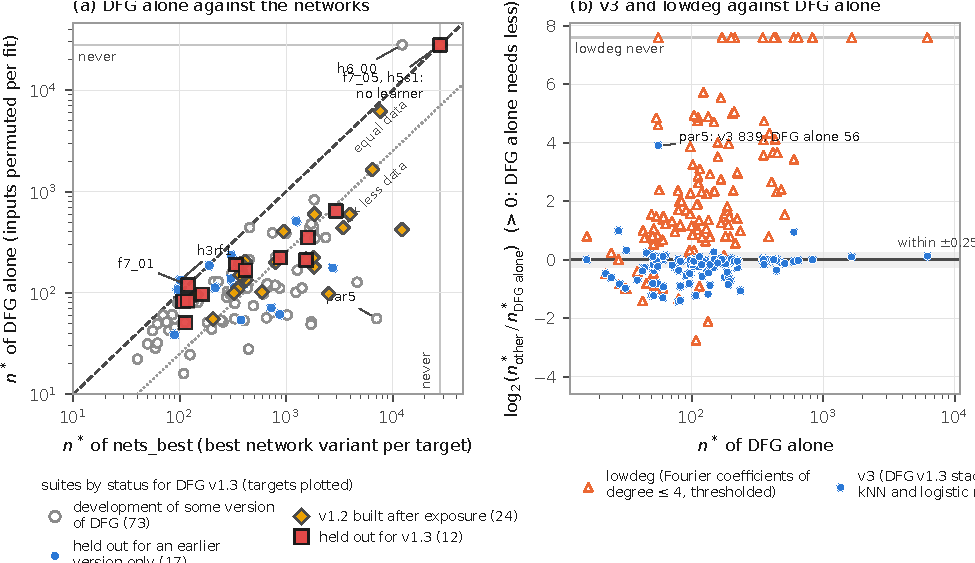
\includegraphics[width=\linewidth]{figures/fig_nstar.pdf}
\caption{(a) $\nstar$ of DFG alone against \code{nets_best} for the 126 targets of the 10 toy suites with network runs \status{Numerical}; colour and marker give the suite's status for DFG v1.3, with \code{dlheld7} as large outlined squares, and ``never'' is drawn at the edge. Below the dashed line DFG needs less data than the best network variant, below the dotted line at least $4\times$ less. (b) For the 134 targets of all 11 suites that DFG alone learns, the $\log_2$ ratio of v3's and of \code{lowdeg}'s $\nstar$ to DFG alone's, against DFG alone's $\nstar$; above 0 DFG alone needs less data; grey: the tie band $\pm0.25$; \code{lowdeg}'s ``never'' at the top. Source: \repo{study/part11/RESULTS.json} via \repo{paper_dfg/make_figures.py}; the plotted points are in \repo{paper_dfg/figures/fig_nstar.json}.}
\label{fig:nstar}
\end{figure}

\paragraph{Pooled} \status{Numerical}.
\begin{itemize}
\item \emph{Against \code{nets_best}:} on the 126 targets of the 10 suites with network runs, DFG's mean is $-1.87$ over the 123 targets both learn, about $3.7\times$ less data (median $-1.65$). Without the held-out \code{dlheld7}, over the 114 in-sample targets, it is $-1.93$ over the 112 both learn. It is clearly better on 117, clearly worse on 2, and needs at least $4\times$ less data on 47 (\cref{fig:nstar}a).
\item \emph{Against single variants:} $-2.04$ against \code{nets_wd}, the one variant run on every suite with network runs (clearly better on 119 of 126, worse on 1), and $-2.64$ against \code{nets} (square loss; 9 suites, 114 targets).
\item \emph{The seven \code{dlheld} suites that Part 10 pooled} (\code{dlheld}, \code{dlheld2}, \dots, \code{dlheld7}, without \code{dlsymdev} and \code{dlfamdev}; 77 targets; for v1.3 only \code{dlheld7} among them is held out): DFG alone is at $-1.71$ and v3 at $-1.87$ against \code{nets_best} on the same targets.
\end{itemize}

\paragraph{By suite} \status{Numerical}. The suite means against \code{nets_best} range from $-2.49$ (\code{dlheld5}) to $-1.27$ (\code{dlheld6}); \code{dlheld7} is at $-1.29$. They are not comparable across suites, because \code{nets_best} minimizes over 2 to 5 variants depending on the suite. Against \code{nets_wd} alone, the three smallest margins are those of the held-out suite and of the two suites held out for v1.1: \code{dlheld2} ($-1.59$), \code{dlheld3} ($-1.60$) and \code{dlheld7} ($-1.62$); the five development suites with network runs give $-1.71$ (\code{dlheld6}) to $-2.45$ (\code{dlsymdev}), and the two exposed suites $-2.05$ and $-2.72$.

\emph{Reading} \status{Heuristic}. Some selection in DFG's favour on the suites it was developed on or exposed to is therefore likely. The suites also differ in kind, though. \code{designed} and \code{random} are small juntas and formulas, \code{dlsymdev} is symmetric, and \code{dlheld2}, \code{dlheld3} and the blind family mix sums, formulas and halfspaces. With 7 to 12 targets per suite, the data do not separate the two explanations. On the held-out suite the margin is about $3\times$ (against \code{nets_wd}), not the $4\times$ of the pooled numbers.

\paragraph{Where DFG is not better} \status{Numerical}. On 9 of the 126 targets with network runs DFG is not clearly better than \code{nets_best}: it is clearly worse on the random formula h3rf1 and on the residue class h6\_00, ties on five (three threshold-like targets, a formula and and3), and no learner learns f7\_05 or h5s1. DFG never learns 4 of the 138 targets (three residue classes mod 3, and h5s1), and neither do v3 and \code{lowdeg} (\cref{app:notwins}). \emph{Reading} \status{Heuristic}: on the small formulas, which v3 and \code{hgb} learn faster, DFG's lack of a clear margin reflects its slowness at small $n$ more than a strength of the networks.

% ------------------------------------------------------------------------------------------------------------------
\subsection{What the portfolio added}\label{sec:res-v3}

On the same training sets and column orders (\cref{sec:refs}; tables in \cref{app:v3}) \status{Numerical}: over the 138 targets, DFG alone's $\nstar$ is lower than v3's on 32 and higher on 101; it equals v3's on 1 (par2), and neither learns 4. Beyond $\pm0.25$ it is lower on 6 and higher on 42. The mean ratio is $+0.19$, so DFG alone needs $1.14\times$ v3's data, and the median is $+0.07$; a two-sided sign test over the 133 targets with unequal $\nstar$ gives $p=1.6\times10^{-9}$. The gap is at small $n$: on the 45 targets that v3 learns by $n=64$, DFG alone's mean is $+0.39$, and v3's test error is lower by more than 0.02 on 63, 64 and 67 of the 138 targets at $n=16$, 32 and 64, on 38 at $n=128$, 17 at 256 and 5 at 512, and on none at $n\ge1024$.
\emph{Reading} \status{Numerical, then Heuristic}. At small $n$ the portfolio's other members carry v3: in Part 10's seed-0 refits the stacker gave the DFG members no weight in 52, 47 and 30 fits at $n=16$, 32 and 64, and on formulas and small thresholds trees, nearest neighbours and logistic regression reach low error with fewer points than DFG needs before its tests admit features. From $n=256$ on, v3 is never worse than its DFG member by more than 0.02, and the DFG members take most of the weight. The reverse, on 3 of the 6 targets where DFG alone needs clearly less data (par3, rf11, par5), is structure that only a fit on all $n$ rows finds: DFG's degree-3 and higher searches need a minimum number of rows and a share of the budget that v3's out-of-fold DFG fits do not have (\cref{app:v3}).

% ------------------------------------------------------------------------------------------------------------------
\subsection{The low-degree algorithm: DFG's characters and test, nothing else}\label{sec:res-lowdeg}

\code{lowdeg} has DFG's global characters up to degree 4 and the same form of union-bound test, applied to the labels, and none of the rest of DFG (\cref{sec:refs}; table in \cref{app:lowdeg}); \cref{fig:nstar}b shows it target by target.

\paragraph{Results} \status{Numerical}.
\begin{itemize}
\item \emph{Against DFG:} pooled over the 138 targets, \code{lowdeg} needs more data. Its mean ratio is $+1.64$ over the 122 targets both learn, about $3.1\times$ more data (median $+1.35$). It is clearly worse on 112 targets and clearly better on 16.
\item \emph{Against the networks} \code{lowdeg} is about even: $-0.16$ against \code{nets_best} over the 112 of 126 targets both learn, clearly better on 53 and clearly worse on 62.
\item \emph{Never learned.} \code{lowdeg} never learns 16 targets: the four that DFG misses and 12 that DFG learns. Of those 12, par5 has degree 5 and is outside \code{lowdeg}'s dictionary; the other 11 are functions of a signed sum, mostly with arbitrary accept sets.
\item \emph{Where \code{lowdeg} is faster.} All 16 such targets are learned at small $n$: DFG needs 22--133 points, \code{lowdeg} 16--61, as on the formulas h3rf0 and h3rf1 and on par4 (28 against 52).
\end{itemize}

\emph{Reading} \status{Heuristic}. DFG's margin over the networks is not explained by its characters and test alone: with them but none of the rest, \code{lowdeg} is at par with the networks. The margin needs what \code{lowdeg} lacks, and the sum blocks are one part of it. They make the signed-sum targets much cheaper to learn, and a few learnable at all within the grid: \code{lowdeg} still learns 39 of the 54 sum-structured targets, more slowly, while DFG without its sum blocks (\code{nosums}, \cref{sec:abl-single}) needs $+0.91$ more in mean $\log_2\nstar$ on the ablation suites and no longer learns band11, h6\_01 and f7\_08. A function of a $k$-input signed sum spreads its Fourier weight over many characters of several degrees, each too weak to pass its own test, while DFG tests the whole block with one $\chi^2$ statistic; the residual rounds let weaker features pass once the stronger ones are fit. On small formulas the comparison runs the other way: at $n\le128$, \code{lowdeg}'s slightly more lenient test, applied to every degree at once on the labels, admits characters at sizes where DFG still keeps few or none.

% ------------------------------------------------------------------------------------------------------------------
\subsection{Input dimension}\label{sec:res-dscale}

DFG and the networks \code{nets} (square loss, the only variant run at every $d$) were run on 7 \code{designed} targets at $d=15$ and 60 and on 4 of them at $d=120$, with seeds 0 and 1, and at $d=30$ with seeds 0, 1 and 2 (\cref{sec:tasks,sec:metrics}). The networks were trained for 20000 steps, 40000 at $d=120$, so one network run, and with it DFG's budget, is twice as large there. \Cref{fig:dscale} plots $\nstar$ with the fitted exponents, and \cref{app:dscale} tabulates them.

\begin{figure}[t]
\centering
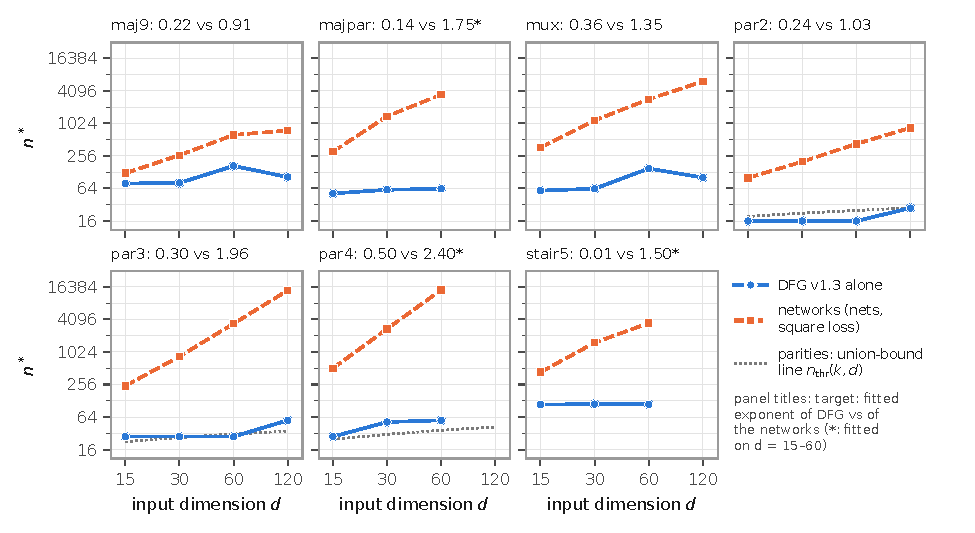
\includegraphics[width=\linewidth]{figures/fig_dscale.pdf}
\caption{$\nstar$ against $d$ (log--log) on the \code{designed} targets with network runs at $d=15$, 60 and 120 (\cref{tab:dscale}) \status{Numerical}. Panel titles give the fitted exponent of DFG v1.3 alone and of the networks \code{nets} ($^\ast$: fitted on $d=15$--60). Dotted, for the $k$-parities: the union-bound line $n_{\rm thr}(k,d)=2\ln(4K\binom{d}{k}/\delta)$ with DFG's $K=4$, $\delta=0.1$ and $c=1$; on the $n$-grid DFG's test passes, when $\bar y$ is near 0, at the first grid point above it (\cref{prop:parity}; where this simple rule misses, and why, is in \cref{app:proof-parity}). Seeds: 2 at $d\ne30$, 3 at $d=30$; the $d=120$ networks were trained for 40000 steps. Source: \repo{study/part11/RESULTS.json} (\texttt{q4\_dscale}) via \repo{paper_dfg/make_figures.py}; the plotted values and $n_{\rm thr}$ are in \repo{paper_dfg/figures/fig_dscale.json}.}
\label{fig:dscale}
\end{figure}

\paragraph{Results} \status{Numerical}.
\begin{itemize}
\item \emph{Exponents.} The least-squares slope of $\log\nstar$ on $\log d$ is 0.01 (stair5) to 0.50 (par4) for DFG v1.3 alone, and 0.91 (maj9) to 2.40 (par4) for the networks, fitted per target on the same $d$.
\item \emph{The gap widens with $d$.} The median $\log_2$ ratio of DFG v1.3 to the networks is $-2.64$ at $d=15$ ($6.2\times$ less data), $-4.19$ at $d=30$ ($18.3\times$), $-4.99$ at $d=60$ ($31.7\times$) and $-5.41$ at $d=120$ ($42.5\times$, 4 targets).
\item \emph{Parities.} DFG's $\nstar$ follows the union-bound line (\cref{fig:dscale}). $n_{\rm thr}$ grows from 19.5 to 27.9 for par2 and from 22.4 to 35.2 for par3 between $d=15$ and 120, and from 24.6 to 36.3 for par4 between $d=15$ and 60. On the grid, DFG's $\nstar$ moves by at most one grid step over the range.
\item \emph{Compute.} DFG's largest fit on these targets uses 0.07, 0.15, 0.18 and 0.18 of one network run at $d=15$, 30, 60 and 120.
\item \emph{The price} \status{Proved, by the code; Numerical}. The enumeration is paid for in FLOPs: an exhaustive degree-$k$ search costs of order $n\binom dk$ FLOPs (\cref{prop:compute}). Within DFG's fixed budget, at $n>512$, the global search can therefore pass no degree-4 character from $d=179$ on and no degree-3 character from $d=630$ on (\cref{prop:floor}; \cref{app:proof-parity,sec:disc-why}).
\end{itemize}

\emph{Reading} \status{Heuristic}.
\begin{itemize}
\item \emph{DFG against gradient descent.} DFG's data cost on a $k$-parity is the union bound's, $2\ln(4K\binom{d}{k}/\delta)$, which grows like $2k\ln d$. The networks' exponents grow with the parity's degree, 1.03, 1.96 and 2.40 for $k=2$, 3 and 4 (par4 fitted on $d=15$--60), as analyses of gradient training on sparse parities lead one to expect \cite{barak2022hidden,abbe2023leap}: exhaustive enumeration pays a logarithm of the dictionary's size, gradient descent a power of $d$.
\item \emph{The size of the factors.} The comparison is with \code{nets}, the plain square-loss network and the weakest variant at $d=30$: on \code{designed}, DFG is at $-2.82$ against \code{nets} and $-2.17$ against \code{nets_wd} (\cref{tab:suites}). The factors are therefore larger than they would be against the best variant. The exponents should be less sensitive to the choice of variant than the factors, but only \code{nets} was run at $d\ne30$.
\end{itemize}

% ------------------------------------------------------------------------------------------------------------------
\subsection{Tabular data and compute}\label{sec:res-tabular}\label{sec:res-compute}

\paragraph{Tabular data} \status{Numerical}. On kr\_vs\_kp and mushroom, the two tabular datasets it can run on (9 cells), DFG is level with gradient boosting in all 9 cells, and with the regularized MLPs and v3 except at the smallest $n$ of kr\_vs\_kp (14.06\% test error against 7.80\% for \code{mlp_reg} and 6.88\% for v3), where they are clearly better; it is nowhere clearly better than the best MLP. Nine cells, with errors near 0 from $n=1000$ on, resolve little. No fit uses more than 0.144 of the standard-task budget. Real-valued data, where Part 7's adaptations of DFG v1.1 were behind a regularized MLP, are not covered (\cref{app:tabular}; \cref{sec:disc-fail}).

\paragraph{Compute} \status{Numerical}. Over all 4730 fits (4334 at $d=30$, 396 at $d\ne30$), the largest uses 0.519 of one network run (h5s5 on \code{dlheld5} at $n=16384$), and none exceeds 0.75. The median fit uses less than 0.001 of a run at $n\le32$, 0.025--0.055 at $n=64$--512 and 0.149 at $n=16384$. CPU time is largest at $n=64$--512 (median 4.2--7.3 seconds per fit), where the cross-validation fits $2F$ small models, each with its own block search. On rough measurements of the same fits DFG alone is faster than v3 (median per-fit CPU ratio 0.06--0.92 at every $n$). Each network fit spends one run by definition, and \code{nets_best} is a hindsight choice among 2 to 5 such runs per target, so ``no more FLOPs'' holds with a wide margin (\cref{app:compute}).

\section{What its parts do}\label{sec:ablations}

DFG v1.3 has many parts (\cref{sec:learner}, \cref{tab:params}). This section asks which of them carry its results. It reports the protocol's 12 ablations (Q5), each DFG alone with one constructor argument changed, and then a post-hoc \emph{core} DFG with nine parts removed at once (\cref{sec:core}). Every run uses the frozen file; only constructor arguments change.

\paragraph{How the runs are compared.} An ablation runs on DFG alone's training sets, column permutations and cross-validation folds, which all come from the fit's random stream. Its $\nstar$ is compared with DFG alone's $\nstar$ computed from the same seeds of DFG alone's own runs. Six ablations (and the core) ran on seeds 0 and 1, six on seed 0 only (\cref{sec:part11}). The ratio is $\log_2(\nstar_{\rm run}/\nstar_{\rm DFG\ alone})$, negative when the run needs less data. A target moves \emph{lower} or \emph{higher} when the ratio is beyond $\mp0.25$; means are over the targets both reach. The five ablation suites hold 65 targets (\code{designed}, \code{dlsymdev}, \code{dlfamdev}, \code{dlheld6}, \code{dlheld7}); only \code{dlheld7} is held out.

\paragraph{Two nulls.} The protocol's null compares DFG alone's seed 1 with its seed 0. Those are different training sets, so it overstates the noise of a paired comparison: it moves 23 of the 65 targets beyond $\pm0.25$. A paired comparison needs a paired null, which was added post hoc: DFG alone refitted on the same training and test sets with another fit stream, so with another column order and other folds and nothing else (\repo{study/part11/interp/ablations/perm_null.py}). The column order is irrelevant to the targets, and no test statistic depends on it, but it can matter through tie-breaking, the block search's orders and the folds. A change that leaves DFG's decisions alone therefore still perturbs its path, and the paired null measures by how much.

\paragraph{Families.} Each target is assigned by hand, from its definition, to one of the nine groups of \cref{sec:interp-atlas} and to three classes (post hoc; \repo{study/part11/interp/ablations/families.py}). \emph{Character targets} are parities, staircases, multiplexers, compositions of parities and majorities and thresholds of a few characters, DNFs, CNFs, decision lists, read-once and random formulas: 71 of the 138 targets, 25 of the 65. \emph{Halfspaces} are majorities and thresholds of a weighted sum, with the dictator, $\mathrm{AND}(x_1,x_2,x_3)$ and an AND of two halfspaces (13 and 7). \emph{Symmetric and mixture targets} are functions of one signed sum, alone or with a parity, a gate, a second sum or an inner term (54 and 33). This class differs from the 54 sum-structured targets of \cref{sec:tasks} by two targets each way: it includes sym8 and sym9, and it counts f7\_01 and fd\_01, thresholds of an unsigned sum, as halfspaces.

\paragraph{Sources.} The summaries are in \repo{study/part11/RESULTS.json} (\texttt{q5\_ablations}, \texttt{q5b\_core}), written by \repo{study/part11/compare_dfg.py}. The groupings, the nulls, the predictions of \cref{sec:abl-test} and the leave-one-in runs of \cref{sec:core} are in \repo{study/part11/interp/ablations/ablations.json}, written by \repo{study/part11/interp/ablations/ablations.py}; the analysis is \repo{study/part11/interp/ablations/ABLATIONS.md}. Models are read from refits of single cells (\repo{study/part11/interp/ablations/refit.py}). A refit uses the instrumented copy of \cref{sec:interp-calib}, so that every feature carries the class that admitted it, and all 36 refits reproduce their run's result file exactly in test error and FLOP count (\repo{study/part11/interp/ablations/results/refits.json}). In four cells the same fit through the evaluation's own loader of the frozen file gives the same model, term by term (\repo{study/part11/interp/ablations/results/refit_crosscheck.json}). The analysis has not been checked by an independent verifier.

% ------------------------------------------------------------------------------------------------------------------
\subsection{Twelve single changes}\label{sec:abl-single}

\begin{table}[t]
\centering{\footnotesize\setlength{\tabcolsep}{2.4pt}\renewcommand{\arraystretch}{1.05}
\begin{tabularx}{\linewidth}{@{}l>{\raggedright\arraybackslash}Xcc>{\raggedright\arraybackslash}p{1.25cm}ccc@{}}
\toprule
run & change & seeds & \hd{all\\(65)} & \hd{newly\\never} & \hd{character\\targets\\(25)} & \hd{halfspaces\\(7)} & \hd{symmetric and\\mixtures\\(33)}\\
\midrule
\code{nosums} & no sum blocks & 0, 1 & \begin{tabular}[t]{@{}c@{}}$+0.91$\\{\scriptsize (2/31) [59]}\end{tabular} & {\scriptsize band11, h6\_01, f7\_08} & \begin{tabular}[t]{@{}c@{}}$+0.16$\\{\scriptsize (1/5) [25]}\end{tabular} & \begin{tabular}[t]{@{}c@{}}$+0.05$\\{\scriptsize (0/1) [7]}\end{tabular} & \begin{tabular}[t]{@{}c@{}}$+1.82$\\{\scriptsize (1/25) [27]}\end{tabular}\\
\code{strict} & stricter tests, $\delta=10^{-4}$ & 0, 1 & \begin{tabular}[t]{@{}c@{}}$+0.06$\\{\scriptsize (9/14) [62]}\end{tabular} & {\scriptsize --} & \begin{tabular}[t]{@{}c@{}}$+0.17$\\{\scriptsize (3/8) [25]}\end{tabular} & \begin{tabular}[t]{@{}c@{}}$-0.23$\\{\scriptsize (4/1) [7]}\end{tabular} & \begin{tabular}[t]{@{}c@{}}$+0.04$\\{\scriptsize (2/5) [30]}\end{tabular}\\
\code{lenient} & more lenient tests, $\delta=0.9$ & 0, 1 & \begin{tabular}[t]{@{}c@{}}$+0.07$\\{\scriptsize (5/13) [62]}\end{tabular} & {\scriptsize --} & \begin{tabular}[t]{@{}c@{}}$+0.12$\\{\scriptsize (2/8) [25]}\end{tabular} & \begin{tabular}[t]{@{}c@{}}$-0.04$\\{\scriptsize (2/1) [7]}\end{tabular} & \begin{tabular}[t]{@{}c@{}}$+0.05$\\{\scriptsize (1/4) [30]}\end{tabular}\\
\code{noeig} & no eigenvector seeds in the block search & 0, 1 & \begin{tabular}[t]{@{}c@{}}$+0.03$\\{\scriptsize (0/1) [62]}\end{tabular} & {\scriptsize --} & \begin{tabular}[t]{@{}c@{}}$+0.00$\\{\scriptsize (0/0) [25]}\end{tabular} & \begin{tabular}[t]{@{}c@{}}$+0.00$\\{\scriptsize (0/0) [7]}\end{tabular} & \begin{tabular}[t]{@{}c@{}}$+0.05$\\{\scriptsize (0/1) [30]}\end{tabular}\\
\code{noblocks} & no linear or spectral block & 0, 1 & \begin{tabular}[t]{@{}c@{}}$-0.02$\\{\scriptsize (6/4) [62]}\end{tabular} & {\scriptsize --} & \begin{tabular}[t]{@{}c@{}}$-0.03$\\{\scriptsize (2/1) [25]}\end{tabular} & \begin{tabular}[t]{@{}c@{}}$-0.19$\\{\scriptsize (3/0) [7]}\end{tabular} & \begin{tabular}[t]{@{}c@{}}$+0.02$\\{\scriptsize (1/3) [30]}\end{tabular}\\
\code{nocomp} & no extension or local classes & 0, 1 & \begin{tabular}[t]{@{}c@{}}$+0.00$\\{\scriptsize (2/2) [62]}\end{tabular} & {\scriptsize --} & \begin{tabular}[t]{@{}c@{}}$+0.02$\\{\scriptsize (1/2) [25]}\end{tabular} & \begin{tabular}[t]{@{}c@{}}$+0.00$\\{\scriptsize (0/0) [7]}\end{tabular} & \begin{tabular}[t]{@{}c@{}}$-0.02$\\{\scriptsize (1/0) [30]}\end{tabular}\\
\code{noweighted} & no weighted blocks & 0 & \begin{tabular}[t]{@{}c@{}}$+0.02$\\{\scriptsize (0/1) [62]}\end{tabular} & {\scriptsize --} & \begin{tabular}[t]{@{}c@{}}$+0.01$\\{\scriptsize (0/0) [25]}\end{tabular} & \begin{tabular}[t]{@{}c@{}}$+0.00$\\{\scriptsize (0/0) [7]}\end{tabular} & \begin{tabular}[t]{@{}c@{}}$+0.03$\\{\scriptsize (0/1) [30]}\end{tabular}\\
\code{nosmalln} & no forced variant, no cross-validation & 0 & \begin{tabular}[t]{@{}c@{}}$+0.12$\\{\scriptsize (0/10) [62]}\end{tabular} & {\scriptsize --} & \begin{tabular}[t]{@{}c@{}}$+0.22$\\{\scriptsize (0/8) [25]}\end{tabular} & \begin{tabular}[t]{@{}c@{}}$-0.03$\\{\scriptsize (0/0) [7]}\end{tabular} & \begin{tabular}[t]{@{}c@{}}$+0.07$\\{\scriptsize (0/2) [30]}\end{tabular}\\
\code{nobg} & no kernel background & 0 & \begin{tabular}[t]{@{}c@{}}$-0.10$\\{\scriptsize (7/3) [62]}\end{tabular} & {\scriptsize --} & \begin{tabular}[t]{@{}c@{}}$-0.07$\\{\scriptsize (3/2) [25]}\end{tabular} & \begin{tabular}[t]{@{}c@{}}$-0.09$\\{\scriptsize (1/0) [7]}\end{tabular} & \begin{tabular}[t]{@{}c@{}}$-0.12$\\{\scriptsize (3/1) [30]}\end{tabular}\\
\code{lsread} & least-squares readout & 0 & \begin{tabular}[t]{@{}c@{}}$-0.01$\\{\scriptsize (2/1) [62]}\end{tabular} & {\scriptsize --} & \begin{tabular}[t]{@{}c@{}}$-0.01$\\{\scriptsize (2/1) [25]}\end{tabular} & \begin{tabular}[t]{@{}c@{}}$+0.00$\\{\scriptsize (0/0) [7]}\end{tabular} & \begin{tabular}[t]{@{}c@{}}$-0.02$\\{\scriptsize (0/0) [30]}\end{tabular}\\
\code{K3} & global search to degree 3 & 0 & \begin{tabular}[t]{@{}c@{}}$+0.02$\\{\scriptsize (2/1) [62]}\end{tabular} & {\scriptsize --} & \begin{tabular}[t]{@{}c@{}}$+0.08$\\{\scriptsize (1/1) [25]}\end{tabular} & \begin{tabular}[t]{@{}c@{}}$-0.05$\\{\scriptsize (1/0) [7]}\end{tabular} & \begin{tabular}[t]{@{}c@{}}$-0.01$\\{\scriptsize (0/0) [30]}\end{tabular}\\
\code{labelnoise} & tests scaled to the labels' noise & 0 & \begin{tabular}[t]{@{}c@{}}$+0.14$\\{\scriptsize (5/15) [62]}\end{tabular} & {\scriptsize --} & \begin{tabular}[t]{@{}c@{}}$+0.23$\\{\scriptsize (2/9) [25]}\end{tabular} & \begin{tabular}[t]{@{}c@{}}$-0.17$\\{\scriptsize (2/0) [7]}\end{tabular} & \begin{tabular}[t]{@{}c@{}}$+0.14$\\{\scriptsize (1/6) [30]}\end{tabular}\\
\midrule
paired null & other column order and folds, same training sets & 0 & \begin{tabular}[t]{@{}c@{}}$+0.00$\\{\scriptsize (0/1) [62]}\end{tabular} & {\scriptsize --} & \begin{tabular}[t]{@{}c@{}}$+0.00$\\{\scriptsize (0/1) [25]}\end{tabular} & \begin{tabular}[t]{@{}c@{}}$+0.00$\\{\scriptsize (0/0) [7]}\end{tabular} & \begin{tabular}[t]{@{}c@{}}$-0.00$\\{\scriptsize (0/0) [30]}\end{tabular}\\
paired null & other column order and folds, same training sets & 0, 1 & \begin{tabular}[t]{@{}c@{}}$-0.02$\\{\scriptsize (2/1) [62]}\end{tabular} & {\scriptsize --} & \begin{tabular}[t]{@{}c@{}}$-0.02$\\{\scriptsize (1/0) [25]}\end{tabular} & \begin{tabular}[t]{@{}c@{}}$+0.00$\\{\scriptsize (0/0) [7]}\end{tabular} & \begin{tabular}[t]{@{}c@{}}$-0.02$\\{\scriptsize (1/1) [30]}\end{tabular}\\
unpaired null & seed 1 against seed 0: other training sets & 1 vs 0 & \begin{tabular}[t]{@{}c@{}}$-0.04$\\{\scriptsize (13/10) [62]}\end{tabular} & {\scriptsize --} & \begin{tabular}[t]{@{}c@{}}$-0.02$\\{\scriptsize (5/4) [25]}\end{tabular} & \begin{tabular}[t]{@{}c@{}}$-0.17$\\{\scriptsize (2/1) [7]}\end{tabular} & \begin{tabular}[t]{@{}c@{}}$-0.04$\\{\scriptsize (6/5) [30]}\end{tabular}\\
\bottomrule
\end{tabularx}
}
\caption{The 12 ablations of Q5 on the 65 targets of the five ablation suites, against DFG alone on the same seeds and training sets \status{Numerical}. Each cell gives the mean $\log_2$ ratio of the run's $\nstar$ to DFG alone's over the targets both learn; below it, the targets on which the run needs clearly less / clearly more data (beyond $\mp0.25$, or only one reaches 10\% error), and in brackets the number both learn. ``Newly never'': targets the run never brings to 10\% error by $n=16384$ while DFG alone does. Class sizes in the header (\cref{sec:ablations}, ``Families''). The three targets that DFG alone never learns (fd\_10, h6\_00, f7\_05) are in no mean. Bottom: the paired null (post hoc), DFG alone refitted on the same training sets with another column order and other cross-validation folds, and the protocol's unpaired null. Sources: \repo{study/part11/RESULTS.json} (\texttt{q5\_ablations}; the pooled column is checked against it) and \repo{study/part11/interp/ablations/ablations.json} via \repo{paper_dfg/make_tables.py}.}
\label{tab:ablations}
\end{table}

\begin{figure}[t]
\centering
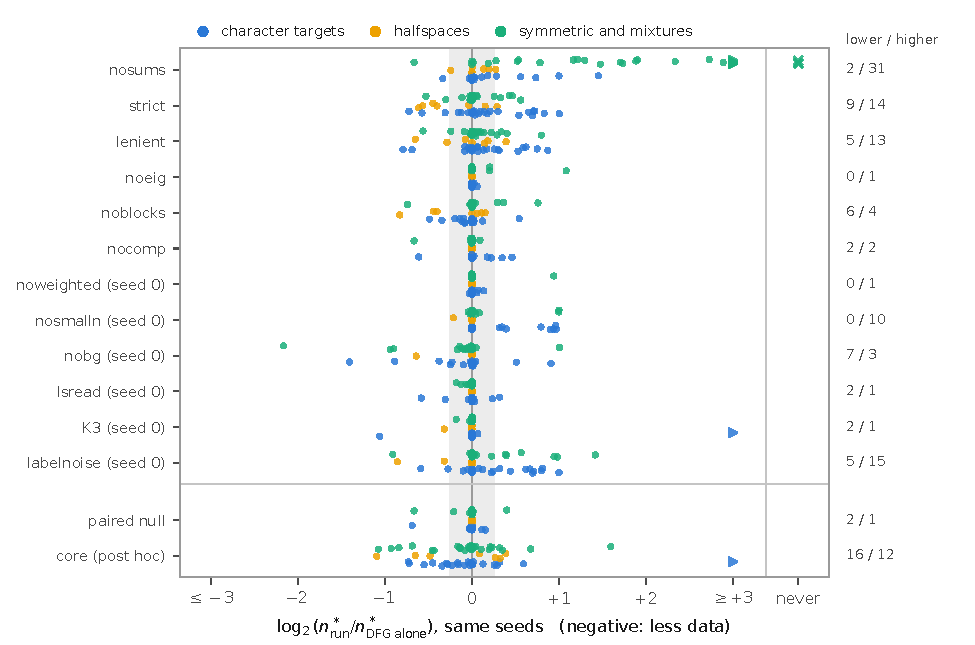
\includegraphics[width=\linewidth]{figures/fig_ablations.pdf}
\caption{Every target of the five ablation suites, one row per run: the $\log_2$ ratio of the run's $\nstar$ to DFG alone's on the same seeds \status{Numerical}. Colour gives the target's class; the grey band is the tie band $\pm0.25$. Ratios beyond $\pm3$ are drawn at the edge (triangles), and ``never'' (the run never reaches 10\% error where DFG alone does) in the right-hand column. Right: the numbers of targets clearly lower / clearly higher. Bottom: the paired null on seeds 0 and 1 (post hoc) and the core DFG of \cref{sec:core} on the same 65 targets (post hoc). Source: \repo{study/part11/interp/ablations/ablations.json} via \repo{paper_dfg/make_figures.py}; the plotted points are in \repo{paper_dfg/figures/fig_ablations.json}.}
\label{fig:ablations}
\end{figure}

\begin{table}[t]
\centering{\footnotesize\setlength{\tabcolsep}{3pt}\renewcommand{\arraystretch}{1.05}
\begin{tabular}{@{}lcccccccc@{}}
\toprule
run & \hd{parities\\(3)} & \hd{stair-\\cases\\(1)} & \hd{half-\\spaces\\(7)} & \hd{compo-\\sitions\\(6)} & \hd{formulas\\(11)} & \hd{random\\formulas\\(4)} & \hd{sym-\\metric\\(12)} & \hd{mixtures\\(21)}\\
\midrule
\code{nosums} & \begin{tabular}[t]{@{}c@{}}$+0.00$\\{\scriptsize (0/0)}\end{tabular} & \begin{tabular}[t]{@{}c@{}}$+0.00$\\{\scriptsize (0/0)}\end{tabular} & \begin{tabular}[t]{@{}c@{}}$+0.05$\\{\scriptsize (0/1)}\end{tabular} & \begin{tabular}[t]{@{}c@{}}$+0.11$\\{\scriptsize (1/1)}\end{tabular} & \begin{tabular}[t]{@{}c@{}}$+0.17$\\{\scriptsize (0/3)}\end{tabular} & \begin{tabular}[t]{@{}c@{}}$+0.36$\\{\scriptsize (0/1)}\end{tabular} & \begin{tabular}[t]{@{}c@{}}$+2.78$\\{\scriptsize (0/9)}\end{tabular} & \begin{tabular}[t]{@{}c@{}}$+1.54$\\{\scriptsize (1/16)}\end{tabular}\\
\code{strict} & \begin{tabular}[t]{@{}c@{}}$+0.40$\\{\scriptsize (0/1)}\end{tabular} & \begin{tabular}[t]{@{}c@{}}$+0.83$\\{\scriptsize (0/1)}\end{tabular} & \begin{tabular}[t]{@{}c@{}}$-0.23$\\{\scriptsize (4/1)}\end{tabular} & \begin{tabular}[t]{@{}c@{}}$+0.09$\\{\scriptsize (2/2)}\end{tabular} & \begin{tabular}[t]{@{}c@{}}$+0.01$\\{\scriptsize (1/2)}\end{tabular} & \begin{tabular}[t]{@{}c@{}}$+0.39$\\{\scriptsize (0/2)}\end{tabular} & \begin{tabular}[t]{@{}c@{}}$-0.01$\\{\scriptsize (0/0)}\end{tabular} & \begin{tabular}[t]{@{}c@{}}$+0.06$\\{\scriptsize (2/5)}\end{tabular}\\
\code{lenient} & \begin{tabular}[t]{@{}c@{}}$-0.26$\\{\scriptsize (1/0)}\end{tabular} & \begin{tabular}[t]{@{}c@{}}$+0.00$\\{\scriptsize (0/0)}\end{tabular} & \begin{tabular}[t]{@{}c@{}}$-0.04$\\{\scriptsize (2/1)}\end{tabular} & \begin{tabular}[t]{@{}c@{}}$+0.36$\\{\scriptsize (0/3)}\end{tabular} & \begin{tabular}[t]{@{}c@{}}$+0.19$\\{\scriptsize (0/5)}\end{tabular} & \begin{tabular}[t]{@{}c@{}}$-0.11$\\{\scriptsize (1/0)}\end{tabular} & \begin{tabular}[t]{@{}c@{}}$+0.07$\\{\scriptsize (0/1)}\end{tabular} & \begin{tabular}[t]{@{}c@{}}$+0.05$\\{\scriptsize (1/3)}\end{tabular}\\
\code{noeig} & \begin{tabular}[t]{@{}c@{}}$+0.00$\\{\scriptsize (0/0)}\end{tabular} & \begin{tabular}[t]{@{}c@{}}$+0.00$\\{\scriptsize (0/0)}\end{tabular} & \begin{tabular}[t]{@{}c@{}}$+0.00$\\{\scriptsize (0/0)}\end{tabular} & \begin{tabular}[t]{@{}c@{}}$+0.00$\\{\scriptsize (0/0)}\end{tabular} & \begin{tabular}[t]{@{}c@{}}$+0.01$\\{\scriptsize (0/0)}\end{tabular} & \begin{tabular}[t]{@{}c@{}}$-0.00$\\{\scriptsize (0/0)}\end{tabular} & \begin{tabular}[t]{@{}c@{}}$+0.02$\\{\scriptsize (0/0)}\end{tabular} & \begin{tabular}[t]{@{}c@{}}$+0.06$\\{\scriptsize (0/1)}\end{tabular}\\
\code{noblocks} & \begin{tabular}[t]{@{}c@{}}$+0.00$\\{\scriptsize (0/0)}\end{tabular} & \begin{tabular}[t]{@{}c@{}}$+0.00$\\{\scriptsize (0/0)}\end{tabular} & \begin{tabular}[t]{@{}c@{}}$-0.19$\\{\scriptsize (3/0)}\end{tabular} & \begin{tabular}[t]{@{}c@{}}$-0.07$\\{\scriptsize (1/0)}\end{tabular} & \begin{tabular}[t]{@{}c@{}}$+0.01$\\{\scriptsize (0/1)}\end{tabular} & \begin{tabular}[t]{@{}c@{}}$-0.12$\\{\scriptsize (1/0)}\end{tabular} & \begin{tabular}[t]{@{}c@{}}$-0.00$\\{\scriptsize (0/0)}\end{tabular} & \begin{tabular}[t]{@{}c@{}}$+0.04$\\{\scriptsize (1/3)}\end{tabular}\\
\code{nocomp} & \begin{tabular}[t]{@{}c@{}}$+0.00$\\{\scriptsize (0/0)}\end{tabular} & \begin{tabular}[t]{@{}c@{}}$+0.00$\\{\scriptsize (0/0)}\end{tabular} & \begin{tabular}[t]{@{}c@{}}$+0.00$\\{\scriptsize (0/0)}\end{tabular} & \begin{tabular}[t]{@{}c@{}}$-0.07$\\{\scriptsize (1/0)}\end{tabular} & \begin{tabular}[t]{@{}c@{}}$+0.08$\\{\scriptsize (0/2)}\end{tabular} & \begin{tabular}[t]{@{}c@{}}$+0.05$\\{\scriptsize (0/0)}\end{tabular} & \begin{tabular}[t]{@{}c@{}}$+0.00$\\{\scriptsize (0/0)}\end{tabular} & \begin{tabular}[t]{@{}c@{}}$-0.03$\\{\scriptsize (1/0)}\end{tabular}\\
\code{noweighted} & \begin{tabular}[t]{@{}c@{}}$+0.00$\\{\scriptsize (0/0)}\end{tabular} & \begin{tabular}[t]{@{}c@{}}$+0.00$\\{\scriptsize (0/0)}\end{tabular} & \begin{tabular}[t]{@{}c@{}}$+0.00$\\{\scriptsize (0/0)}\end{tabular} & \begin{tabular}[t]{@{}c@{}}$+0.00$\\{\scriptsize (0/0)}\end{tabular} & \begin{tabular}[t]{@{}c@{}}$+0.02$\\{\scriptsize (0/0)}\end{tabular} & \begin{tabular}[t]{@{}c@{}}$+0.00$\\{\scriptsize (0/0)}\end{tabular} & \begin{tabular}[t]{@{}c@{}}$+0.00$\\{\scriptsize (0/0)}\end{tabular} & \begin{tabular}[t]{@{}c@{}}$+0.04$\\{\scriptsize (0/1)}\end{tabular}\\
\code{nosmalln} & \begin{tabular}[t]{@{}c@{}}$+0.26$\\{\scriptsize (0/1)}\end{tabular} & \begin{tabular}[t]{@{}c@{}}$+0.00$\\{\scriptsize (0/0)}\end{tabular} & \begin{tabular}[t]{@{}c@{}}$-0.03$\\{\scriptsize (0/0)}\end{tabular} & \begin{tabular}[t]{@{}c@{}}$+0.38$\\{\scriptsize (0/3)}\end{tabular} & \begin{tabular}[t]{@{}c@{}}$+0.15$\\{\scriptsize (0/3)}\end{tabular} & \begin{tabular}[t]{@{}c@{}}$+0.22$\\{\scriptsize (0/1)}\end{tabular} & \begin{tabular}[t]{@{}c@{}}$+0.11$\\{\scriptsize (0/1)}\end{tabular} & \begin{tabular}[t]{@{}c@{}}$+0.05$\\{\scriptsize (0/1)}\end{tabular}\\
\code{nobg} & \begin{tabular}[t]{@{}c@{}}$+0.00$\\{\scriptsize (0/0)}\end{tabular} & \begin{tabular}[t]{@{}c@{}}$+0.04$\\{\scriptsize (0/0)}\end{tabular} & \begin{tabular}[t]{@{}c@{}}$-0.09$\\{\scriptsize (1/0)}\end{tabular} & \begin{tabular}[t]{@{}c@{}}$-0.12$\\{\scriptsize (1/0)}\end{tabular} & \begin{tabular}[t]{@{}c@{}}$-0.10$\\{\scriptsize (1/1)}\end{tabular} & \begin{tabular}[t]{@{}c@{}}$+0.00$\\{\scriptsize (1/1)}\end{tabular} & \begin{tabular}[t]{@{}c@{}}$-0.04$\\{\scriptsize (0/0)}\end{tabular} & \begin{tabular}[t]{@{}c@{}}$-0.16$\\{\scriptsize (3/1)}\end{tabular}\\
\code{lsread} & \begin{tabular}[t]{@{}c@{}}$+0.00$\\{\scriptsize (0/0)}\end{tabular} & \begin{tabular}[t]{@{}c@{}}$+0.00$\\{\scriptsize (0/0)}\end{tabular} & \begin{tabular}[t]{@{}c@{}}$+0.00$\\{\scriptsize (0/0)}\end{tabular} & \begin{tabular}[t]{@{}c@{}}$+0.06$\\{\scriptsize (0/1)}\end{tabular} & \begin{tabular}[t]{@{}c@{}}$-0.06$\\{\scriptsize (2/0)}\end{tabular} & \begin{tabular}[t]{@{}c@{}}$-0.01$\\{\scriptsize (0/0)}\end{tabular} & \begin{tabular}[t]{@{}c@{}}$-0.00$\\{\scriptsize (0/0)}\end{tabular} & \begin{tabular}[t]{@{}c@{}}$-0.02$\\{\scriptsize (0/0)}\end{tabular}\\
\code{K3} & \begin{tabular}[t]{@{}c@{}}$+1.00$\\{\scriptsize (0/1)}\end{tabular} & \begin{tabular}[t]{@{}c@{}}$+0.07$\\{\scriptsize (0/0)}\end{tabular} & \begin{tabular}[t]{@{}c@{}}$-0.05$\\{\scriptsize (1/0)}\end{tabular} & \begin{tabular}[t]{@{}c@{}}$+0.00$\\{\scriptsize (0/0)}\end{tabular} & \begin{tabular}[t]{@{}c@{}}$-0.00$\\{\scriptsize (0/0)}\end{tabular} & \begin{tabular}[t]{@{}c@{}}$-0.26$\\{\scriptsize (1/0)}\end{tabular} & \begin{tabular}[t]{@{}c@{}}$+0.00$\\{\scriptsize (0/0)}\end{tabular} & \begin{tabular}[t]{@{}c@{}}$-0.01$\\{\scriptsize (0/0)}\end{tabular}\\
\code{labelnoise} & \begin{tabular}[t]{@{}c@{}}$+0.00$\\{\scriptsize (0/0)}\end{tabular} & \begin{tabular}[t]{@{}c@{}}$+0.70$\\{\scriptsize (0/1)}\end{tabular} & \begin{tabular}[t]{@{}c@{}}$-0.17$\\{\scriptsize (2/0)}\end{tabular} & \begin{tabular}[t]{@{}c@{}}$+0.11$\\{\scriptsize (1/1)}\end{tabular} & \begin{tabular}[t]{@{}c@{}}$+0.33$\\{\scriptsize (1/6)}\end{tabular} & \begin{tabular}[t]{@{}c@{}}$+0.19$\\{\scriptsize (0/1)}\end{tabular} & \begin{tabular}[t]{@{}c@{}}$+0.10$\\{\scriptsize (0/1)}\end{tabular} & \begin{tabular}[t]{@{}c@{}}$+0.15$\\{\scriptsize (1/5)}\end{tabular}\\
\midrule
paired null (0, 1) & \begin{tabular}[t]{@{}c@{}}$-0.00$\\{\scriptsize (0/0)}\end{tabular} & \begin{tabular}[t]{@{}c@{}}$+0.00$\\{\scriptsize (0/0)}\end{tabular} & \begin{tabular}[t]{@{}c@{}}$+0.00$\\{\scriptsize (0/0)}\end{tabular} & \begin{tabular}[t]{@{}c@{}}$-0.11$\\{\scriptsize (1/0)}\end{tabular} & \begin{tabular}[t]{@{}c@{}}$+0.02$\\{\scriptsize (0/0)}\end{tabular} & \begin{tabular}[t]{@{}c@{}}$-0.00$\\{\scriptsize (0/0)}\end{tabular} & \begin{tabular}[t]{@{}c@{}}$-0.02$\\{\scriptsize (0/0)}\end{tabular} & \begin{tabular}[t]{@{}c@{}}$-0.01$\\{\scriptsize (1/1)}\end{tabular}\\
paired null (0) & \begin{tabular}[t]{@{}c@{}}$-0.00$\\{\scriptsize (0/0)}\end{tabular} & \begin{tabular}[t]{@{}c@{}}$+0.00$\\{\scriptsize (0/0)}\end{tabular} & \begin{tabular}[t]{@{}c@{}}$+0.00$\\{\scriptsize (0/0)}\end{tabular} & \begin{tabular}[t]{@{}c@{}}$-0.02$\\{\scriptsize (0/0)}\end{tabular} & \begin{tabular}[t]{@{}c@{}}$+0.02$\\{\scriptsize (0/1)}\end{tabular} & \begin{tabular}[t]{@{}c@{}}$-0.00$\\{\scriptsize (0/0)}\end{tabular} & \begin{tabular}[t]{@{}c@{}}$+0.00$\\{\scriptsize (0/0)}\end{tabular} & \begin{tabular}[t]{@{}c@{}}$-0.00$\\{\scriptsize (0/0)}\end{tabular}\\
unpaired null & \begin{tabular}[t]{@{}c@{}}$-0.33$\\{\scriptsize (1/0)}\end{tabular} & \begin{tabular}[t]{@{}c@{}}$+0.01$\\{\scriptsize (0/0)}\end{tabular} & \begin{tabular}[t]{@{}c@{}}$-0.17$\\{\scriptsize (2/1)}\end{tabular} & \begin{tabular}[t]{@{}c@{}}$+0.17$\\{\scriptsize (1/2)}\end{tabular} & \begin{tabular}[t]{@{}c@{}}$-0.01$\\{\scriptsize (2/1)}\end{tabular} & \begin{tabular}[t]{@{}c@{}}$-0.07$\\{\scriptsize (1/1)}\end{tabular} & \begin{tabular}[t]{@{}c@{}}$+0.01$\\{\scriptsize (1/1)}\end{tabular} & \begin{tabular}[t]{@{}c@{}}$-0.06$\\{\scriptsize (5/4)}\end{tabular}\\
\midrule
core (post hoc) & \begin{tabular}[t]{@{}c@{}}$+2.01$\\{\scriptsize (0/1)}\end{tabular} & \begin{tabular}[t]{@{}c@{}}$-0.08$\\{\scriptsize (0/0)}\end{tabular} & \begin{tabular}[t]{@{}c@{}}$-0.17$\\{\scriptsize (3/3)}\end{tabular} & \begin{tabular}[t]{@{}c@{}}$-0.15$\\{\scriptsize (3/1)}\end{tabular} & \begin{tabular}[t]{@{}c@{}}$-0.04$\\{\scriptsize (2/2)}\end{tabular} & \begin{tabular}[t]{@{}c@{}}$-0.27$\\{\scriptsize (2/1)}\end{tabular} & \begin{tabular}[t]{@{}c@{}}$-0.03$\\{\scriptsize (0/0)}\end{tabular} & \begin{tabular}[t]{@{}c@{}}$-0.05$\\{\scriptsize (6/4)}\end{tabular}\\
\bottomrule
\end{tabular}
}
\caption{The ablations by target family (the groups of \cref{sec:interp-atlas}; group sizes in the header) on the 65 targets of the five ablation suites \status{Numerical; families post hoc}. Each cell: mean $\log_2$ ratio over the targets both learn, and the targets clearly lower / clearly higher. The symmetric group holds the three targets no learner learns, so its means are over 9 targets (6 under \code{nosums}). Bottom: the paired and unpaired nulls, and the core DFG on the same 65 targets (post hoc). Source: \repo{study/part11/interp/ablations/ablations.json}.}
\label{tab:abl-family}
\end{table}

\Cref{tab:ablations,tab:abl-family} and \cref{fig:ablations} give the results.

\paragraph{The paired null} \status{Numerical; post hoc}. On seed 0 the re-permuted fits move 1 of the 65 targets beyond $\pm0.25$ (dlist5, $+0.39$), and 10 of the 65 ratios are not zero; the mean $|\text{ratio}|$ is 0.012. On seeds 0 and 1 they move 3 (andxor $-0.69$, thrsum $-0.66$, h6\_07 $+0.40$), with mean $|\text{ratio}|$ 0.038. Over all 138 targets of the 11 suites they move 8 on seeds 0 and 1 (mean $|\text{ratio}|$ 0.040). The unpaired null moves 23 to 31 of the 65 targets, depending on the pair of seeds.

\paragraph{What carries the results} \status{Numerical}.
\begin{itemize}
\item \emph{Sum blocks.} Without them (\code{nosums}) the mean ratio is $+0.91$ over the 59 targets both learn, with 31 clearly higher and 2 lower, and DFG no longer learns band11, h6\_01 and f7\_08. The cost falls on the symmetric targets ($+2.78$, 9 of the 9 that DFG alone learns move, 3 of them to ``never'') and the mixtures ($+1.54$, 16 of 21 higher). Character targets lose little ($+0.16$; rand3, parmaj, h6\_05, fd\_07 and dnf3 move up). They are of the kinds the atlas found encoded in part by blocks before their characters are all detectable: parmaj by two folded blocks, formulas by the blocks of a clause or term (\cref{sec:interp-atlas}). The two seeds agree: 27 targets move up on both and none in opposite directions.
\item \emph{Tests scaled to the residual} (\code{labelnoise}, $+0.14$; 15 higher, 5 lower) and \emph{the small-$n$ machinery} (\code{nosmalln}, $+0.12$; 10 higher, none lower) come next, mostly on character targets (\cref{sec:abl-smalln,sec:abl-label}).
\end{itemize}

\paragraph{What moves both ways} \status{Numerical}. The two test levels, the kernel background and the linear and spectral blocks move 10 to 23 targets each, in both directions, with means between $-0.10$ and $+0.07$. Halfspaces gain from \code{strict} ($-0.23$), \code{noblocks} ($-0.19$) and \code{labelnoise} ($-0.17$), three changes that keep features out of the model at small $n$ (\cref{sec:abl-test}). For \code{strict} and \code{lenient}, most movements are one grid step on one seed: 24 and 22 targets move on one seed only, 5 and 4 on both.

\paragraph{What can be removed} \status{Numerical}. Five parts stay within the paired null, or close to it, on these 65 targets:
\begin{itemize}
\item the eigenvector seeds of the block search (\code{noeig}): 1 target moves, h6\_10 ($+1.08$);
\item the extension and local classes (\code{nocomp}): 4 move, among them andxor and thrsum, which the paired null also moves by as much;
\item the weighted blocks (\code{noweighted}): 1 moves, h6\_10 again ($+0.94$), the target they were designed after (\cref{tab:status});
\item the logistic refinement (\code{lsread}): 3 move, by at most 0.58;
\item the search of degrees 4--6 (\code{K3}): 3 move, of which only par4 by much ($+3.01$; \cref{sec:abl-k3}).
\end{itemize}
Their mean $|\text{ratio}|$ is 0.020--0.075, against 0.012 and 0.038 for the paired null on one and two seeds.

\emph{Reading} \status{Heuristic}. On these suites DFG's results come from the sum blocks, with the residual scaling of the tests and the small-$n$ machinery as smaller contributors. Five parts can each be removed without a change larger than an arbitrary perturbation of the path produces. Two qualifications apply. The suites contain few targets that need those parts: one pure 4-parity, no dense halfspace on more than 13 inputs, no degree-5 parity. And the parts are removed one at a time, so they may substitute for one another. \Cref{sec:core} removes them together.

% ------------------------------------------------------------------------------------------------------------------
\subsection{The test or the search}\label{sec:abl-test}

\code{strict} ($\delta=10^{-4}$) and \code{lenient} ($\delta=0.9$) move the log term of every test by $+6.91$ and $-2.20$ nats. If a target's data cost is set by a test, its $\nstar$ should move by a predictable amount; if it is set by the search, it should not move. \Cref{sec:interp-when} goes through these two runs target by target (\cref{fig:dyn-when}); this subsection summarizes them and adds the refits behind the asymmetry between the two.

\paragraph{Parities: the test, exactly} \status{Numerical}. By \cref{prop:parity}, a $k$-parity passes round 0's test exactly when $n(1-\bar y^2)>n_{\rm thr}(k,d)$, and $n_{\rm thr}$ moves by $+13.8$ and $-4.4$ rows with $\delta$. At $d=30$ it moves from 22.3, 26.8 and 30.6 ($k=2,3,4$) to 36.1, 40.6 and 44.4 under \code{strict}, and to 17.9, 22.4 and 26.2 under \code{lenient}. Applied seed by seed to each training set's own $\bar y$, this predicts the measured changes of $\nstar$ to within 0.03: par3 $+0.98$ against $+1.00$ under \code{strict}, and 0 against 0 under \code{lenient}; par4 $+0.20$ against $+0.21$, and $-0.79$ against $-0.79$. par2 moves under neither, because the forced variant fits it at $n=16$, below every $n_{\rm thr}$ here, and the cross-validation's choice does not depend on $\delta$.

\paragraph{Other character targets} \status{Numerical}. By \cref{prop:nglob}(b), $n_{\rm glob}$ is proportional to the log term, so \code{strict} should raise it by $+0.54$ to $+0.86$ doublings (degree 4 to degree 1), and \code{lenient} lower it by $-0.22$ to $-0.43$. \code{strict} raises $\nstar$ beyond 0.25 on 8 of the 25 character targets (par3, stair5, rand3, rand2, majpar, sparsepoly, h6\_03, h6\_05), and their first fit moves one grid step. \code{lenient} is not the mirror image: it lowers $\nstar$ on 2 targets (par4, rand2) and raises it on 8 (andxor, majpar, fd\_00, mux, fd\_07, dlist5, h6\_05, f7\_02). Two things cause the asymmetry. Most of these targets are first fitted at $n=32$--64, often by the forced variant. And the test most sensitive to $\delta$ is the linear block's, whose threshold on 30 inputs (\cref{eq:lintest}) is 51.2 at $\delta=0.1$, 33.8 at $0.9$ and 81.7 at $10^{-4}$. Refits show both.
\begin{itemize}
\item \emph{majpar at $n=64$} (seed 0). With $\delta=0.1$ nothing passes in round 0. The forced variant adds $\chi_{\{1,2\}}$ and then $\chi_{\{3,4\}}$, and $\chi_{\{5,6\}}$ passes its own test in round 2: error 0.067. With $\delta=0.9$, $\chi_{\{1,2\}}$ passes in round 0 and the linear block enters with 30 degree-1 characters, none of them in majpar's Fourier support; then nothing passes, and the error is 0.341. With $\delta=10^{-4}$ the forced pairs are the same, but $\chi_{\{5,6\}}$ fails its test: error 0.269.
\item \emph{f7\_02 at $n=128$} (a DNF of three terms, seed 1), the other direction. With $\delta=0.1$ the linear block enters, and the default variant is kept: error 0.202. With $\delta=10^{-4}$ nothing passes. The forced variant guesses the blocks $(x_2-x_6-x_8)$ and $(-x_3+x_5+x_7)$, two of the DNF's terms; the third term's block then passes its test, and the cross-validation keeps the forced variant: error 0.
\end{itemize}

\paragraph{Halfspaces and sum targets} \status{Numerical}. Halfspaces gain from a stricter test ($-0.23$; 4 of 7 lower). On f7\_01 at $n=128$, a degree-1 character that passes its own test first takes part of the exact block's signal in the block's second test, and with $\delta=10^{-4}$ the block enters instead (\cref{sec:interp-when}). On the 33 symmetric and mixture targets the class means are $+0.04$ and $+0.05$ (30 learned; 5 and 4 higher, 2 and 1 lower). At the true block's detection point $n_{\rm detect}$ (Part 10's block statistics, re-thresholded for each $\delta$), \code{strict} moves the block threshold by $+0.20$ to $+0.30$ doublings of $n$. On the 7 targets whose $\nstar$ lies a doubling or more beyond $n_{\rm detect}$, it changes $\nstar$ by at most 0.05. On the other 23, $\nstar$ lies less than a doubling beyond $n_{\rm detect}$ (for 18 at or below it), and the grid cannot separate the test from the search.

\emph{Reading} \status{Heuristic}. For character targets the round-0 test is binding when the first fit comes from it: exactly for the parities, within a grid step for staircases and small formulas. Where the first fit is the forced variant's, $\delta$ acts through the linear block and the cross-validation instead, and the sign of its effect does not follow from the test alone. For the sum targets the test is not binding: once the search proposes the block, the block passes far above its threshold (9 to 71 times for par4 in \cref{sec:abl-k3}). This agrees with Part 10's reading that the search, not the test, sets their data cost \cite{portfoliolearner2026}.

% ------------------------------------------------------------------------------------------------------------------
\subsection{Degree 4 without the degree-4 search}\label{sec:abl-k3}

\code{K3} sets $K=K_{\rm hi}=3$: the global search stops at degree 3, and the degree-5/6 search is off. $K$ also enters every class's union bound through $\ln(4KN/\delta)$ (\cref{eq:chartest}), so every test becomes 0.29 nats more lenient. On the 65 targets \code{K3} moves 3 (\cref{tab:ablations}).

\paragraph{par4} \status{Numerical; refits, seed 0}. Under \code{K3}, par4's test error is 0.49--0.50 at $n\le256$, 0 at 512, 0.50 at 1024, 0 at 2048 and 4096, and 0.49--0.50 at 8192 and 16384. In the three fitted cells the model is a folded block on the parity's four inputs, admitted in round 0 by an additive block search: $|{-x_1}-x_2-x_3-x_4|$ at 512, $|x_1-x_2+x_3+x_4|$ at 2048 and $|x_1-x_2-x_3+x_4|$ at 4096, at 9.0, 34.5 and 70.9 times its threshold. A $k$-parity is a function of any signed sum of its $k$ inputs, so one folded block represents it exactly (\cref{prop:blocks}). In the four empty cells the round-0 block searches' best candidates stand at 0.13--0.45 of their thresholds, and the model is the constant and the background. With the degree-4 search, $\chi_{\{1,2,3,4\}}$ passes its round-0 test from $n=64$ on (\cref{prop:parity}).

\paragraph{mux and andxor} \status{Numerical; refits, seed 0}. These two targets have degree-4 coefficients of 0.75 and 0.5. Their test error under \code{K3} equals DFG alone's at every $n$, but the models differ.
\begin{itemize}
\item mux at $n=256$: DFG alone's largest term is $\chi_{\{1,2,3,4\}}$ (share 0.51), admitted by the degree-4 test in round 0. \code{K3} holds no degree-4 character; it has the blocks $(-x_1-x_2-x_3+x_4)$ and $(x_1+x_2+x_3+3x_4)$, and $\chi_{\{1,2,3\}}$ from the two-input extension of $\chi_{\{1\}}$.
\item andxor at $n=256$: DFG alone holds its exact expansion $\chi_{\{1,2\}}$, $\chi_{\{3,4\}}$, $\chi_{\{1,2,3,4\}}$. \code{K3} holds the two pair characters and the weighted block $(x_1+x_2-3x_3x_4)$.
\end{itemize}

\paragraph{rand1, $-1.06$} \status{Numerical; refit, seed 0, $n=64$}. With $K=4$, round 0 admits the linear block (30 degree-1 characters, one of them relevant), and the forced variant then guesses $\chi_{\{4,12,17\}}$: error 0.412. With $K=3$, $\chi_{\{1\}}$ passes its own, slightly more lenient test, so the linear block does not enter. The forced guess is then $\chi_{\{1,4,6\}}$, the local class adds $\chi_{\{4,6\}}$, and a block $(x_3-x_5)$ follows: error 0. This difference comes from $K$ in the union bound, not from the degree-4 search.

\emph{Reading} \status{Heuristic}. The degree-4 search is redundant where a target's degree-4 characters share their inputs with lower-degree structure: blocks on those inputs, and the extension and local classes, reach them. It is indispensable for a degree-4 parity with no lower-degree footprint. The block test would admit the exact block from small $n$ on, but the block search starts from degree-1 and degree-2 statistics (\cref{prop:blocks}), which are zero for such a parity, so it finds the four inputs only by chance. The ablation suites contain one such target. \Cref{sec:core} adds three more.

% ------------------------------------------------------------------------------------------------------------------
\subsection{The small-\texorpdfstring{$n$}{n} machinery and the background}\label{sec:abl-smalln}

The atlas computed two counterfactuals on its 37 targets (\cref{sec:interp-atlas}): the variant DFG's cross-validation did not choose, refitted on the same rows, and each fitted model without its kernel background. \code{nosmalln} and \code{nobg} run them as learners, and on the 21 targets the ablation suites share with the atlas the two agree.

\paragraph{No forced variant, no cross-validation} \status{Numerical}. \code{nosmalln} fits the default variant on all $n$ rows. At $d=30$ it can differ from the atlas's ``always default'' refit only in the degree-5/6 subsample sizes (\cref{prop:compute}). Its seed-0 test error equals that refit's in all 126 cells with $n\le512$. Over the 65 targets, the mean test error rises by 0.012, 0.007, 0.022, 0.009 and 0.004 at $n=16$, 32, 64, 128 and 256, and by nothing from 512 on. $\nstar$ rises on 10 targets and falls on none (mean $+0.12$). Since \code{nosmalln} is the default variant, every cell where DFG alone does better is one where DFG alone kept the forced variant. The first fits lost this way are par2 and rand2 at $n=16$, majpar at 32 and 64, mux and sym7 at 64, fd\_04 at 128 and f7\_02 at 256. Each comes back one grid step later. Over the atlas's 222 cells, DFG's choice has mean test error 0.2257, always taking the default 0.2319, always taking the forced variant 0.2256, and the better of the two in each cell 0.2111 (\cref{sec:interp-atlas}).

\paragraph{No kernel background} \status{Numerical}. The background is added after the weights are fitted. A fitted model without it therefore gives exactly DFG's prediction without it for the same variant. The ablation can differ from that only where the cross-validation chooses another variant, because the fold fits lose their background too. \code{nobg}'s seed-0 error equals the atlas's model-without-background error in 224 of 231 cells. The other 7 are all at $n\le128$, so in each of them the choice changed. One is refitted: f7\_11 at $n=16$. DFG alone keeps the default variant there (held-out errors 6 and 3), the constant plus the background, with test error 0.301. Without the background, the default variant's held-out errors rise to 13, the forced variant is kept, and its model $\chi_{\{11\}}$, $\chi_{\{8\}}$ has error 0.077. Over the 65 targets the mean error rises by 0.015 and 0.016 at $n=16$ and 32, and falls by 0.009, 0.002, 0.003 and 0.002 at 64, 128, 256 and 512. $\nstar$ falls on 7 targets and rises on 3 (mean $-0.10$); f7\_11 falls most ($-2.17$).

\emph{Reading} \status{Heuristic}. With nothing else in the model, at $n=16$--32, the background is a Hebbian classifier, and it helps targets with a strong degree-1 part. From $n=64$ on it adds the noise of 30 residual correlations to a model that already fits. Through the cross-validation it also makes the default variant look better than it is, so the forced variant's right guesses are kept less often. Most $\nstar$ lie at 64--512, so the background costs data on balance on these suites.

% ------------------------------------------------------------------------------------------------------------------
\subsection{Tests scaled to the residual}\label{sec:abl-label}

\code{labelnoise} replaces $s$ by 1 in every threshold, so the tests are scaled to the labels' noise instead of the residual's. (The subsampled searches keep their subsample's root mean square, and a block's second test, on the projected residual, keeps that residual's variance.) In round 0 the residual is $y-\bar y$, with variance $1-\bar y^2$, and after the first features fit it shrinks. By \cref{prop:nglob}(c), characters admitted after round 0 enter 1.4--3.7 doublings below $n_{\rm glob}$ (class medians), mainly because the residual variance there is 3.2--19 times smaller (class medians; \cref{prop:nglob}, ``Checks'').

\paragraph{Results} \status{Numerical}. The mean ratio is $+0.14$ (15 higher, 5 lower). By family: formulas $+0.33$ (6 of 11 higher), the staircase $+0.70$, random formulas $+0.19$, mixtures $+0.15$ (5 of 21), compositions $+0.11$, symmetric targets $+0.10$, parities 0, halfspaces $-0.17$ (\cref{tab:abl-family}). The mean test error rises by 0.024 at $n=128$ (18 targets higher by more than 0.02, 2 lower) and by 0.013 at 256, and by at most 0.004 in absolute value elsewhere. Two refits at $n=128$ (seed 0) show the two ways the scaling matters.
\begin{itemize}
\item \emph{Later rounds}, rand3. DFG alone admits $\chi_{\{5,6\}}$ in round 0 ($s=1.00$), $\chi_{\{4,5,6\}}$ by the one-input extension in round 1 ($s=0.84$), two local characters in round 2 ($s=0.77$) and modulated blocks in rounds 3 and 4: error 0.049. With $s=1$ the first round is the same, but nothing passes in round 1, and the fit stops: error 0.317.
\item \emph{Biased labels}, far9 $=[|x_1+\dots+x_9|\ge5]$, whose round-0 residual has $s=0.71$. DFG alone admits the folded block $|x_1+\dots+x_9|$ and a spectral feature in round 0: error 0.006. With $s=1$ the thresholds are 1.4 times higher, nothing passes, and the model is the constant and the background: error 0.181.
\end{itemize}

\emph{Reading} \status{Heuristic}. The residual scaling is what makes the growth greedy in the sense of DFG's design: each round's tests are calibrated to the noise left after the previous round, so weaker features pass once stronger ones are in. Its cost on these targets is modest, because the features that bring most targets below 10\% error enter in round 0 (\cref{sec:interp-order}). It is larger for formulas and staircases, whose later characters build on the first ones, and for targets with biased labels.

% ------------------------------------------------------------------------------------------------------------------
\subsection{A core DFG (post hoc)}\label{sec:core}

\emph{Everything in this subsection is post hoc.} The protocol's addendum (\repo{study/part11/PROTOCOL.md}) was written after every pre-registered result had been read, to ask whether the parts that are removable one at a time can be removed together. The \code{core} run keeps the global characters of degree at most 3; the unweighted signed-sum blocks, searched from pairs and single inputs, with their modulated, product, split, beam and forced moves; the union-bound tests scaled to the residual; least squares; and the small-$n$ cross-validation. It removes nine parts: the linear and spectral blocks, the extension and local classes, the degree-4 to degree-6 searches, the weighted blocks, the eigenvector seeds, the logistic refinement and the kernel background. Through $K=3$, every test is also 0.29 nats more lenient. The code is the frozen file, with the constructor arguments \code{readout="ls"}, \code{sum_inner=False}, \code{sum_seeds=(0,3,2)}, \code{blocks=False}, \code{max_ext_bases=0}, \code{local_max=0}, \code{K=3}, \code{K_hi=3} and \code{background=False}. It ran on all 11 suites, with seeds 0 and 1 and the standard grid. Its definition used the ablations' results on all five ablation suites, \code{dlheld7} included, so no suite is held out for it.

\begin{table}[t]
\centering{\footnotesize\setlength{\tabcolsep}{3pt}\renewcommand{\arraystretch}{1.05}
\begin{tabular}{@{}llccccc@{}}
\toprule
suite & status for DFG v1.3 & targets & \hd{core vs\\DFG alone} & \hd{newly\\never} & \hd{core vs\\\code{nets_best}} & \hd{DFG alone vs\\\code{nets_best}}\\
\midrule
\code{designed} & development & 21 & \begin{tabular}[t]{@{}c@{}}$+0.11$\\{\scriptsize(8/5) [21]}\end{tabular} & -- & \begin{tabular}[t]{@{}c@{}}$-2.03$\\{\scriptsize(20/1) [21]}\end{tabular} & \begin{tabular}[t]{@{}c@{}}$-2.14$\\{\scriptsize(20/0) [21]}\end{tabular}\\
\code{random} & development & 20 & \begin{tabular}[t]{@{}c@{}}$+0.26$\\{\scriptsize(3/3) [20]}\end{tabular} & -- & \begin{tabular}[t]{@{}c@{}}$-1.78$\\{\scriptsize(19/1) [20]}\end{tabular} & \begin{tabular}[t]{@{}c@{}}$-2.04$\\{\scriptsize(20/0) [20]}\end{tabular}\\
\code{dlheld} & development & 12 & \begin{tabular}[t]{@{}c@{}}$+0.15$\\{\scriptsize(2/3) [11]}\end{tabular} & par5 & \begin{tabular}[t]{@{}c@{}}$-1.57$\\{\scriptsize(8/2) [11]}\end{tabular} & \begin{tabular}[t]{@{}c@{}}$-2.17$\\{\scriptsize(11/0) [12]}\end{tabular}\\
\code{dlheld2} & \begin{tabular}[t]{@{}l@{}}held out for\\v1.1 only\end{tabular} & 7 & \begin{tabular}[t]{@{}c@{}}$+0.46$\\{\scriptsize(0/3) [7]}\end{tabular} & -- & \begin{tabular}[t]{@{}c@{}}$-1.15$\\{\scriptsize(6/1) [7]}\end{tabular} & \begin{tabular}[t]{@{}c@{}}$-1.62$\\{\scriptsize(7/0) [7]}\end{tabular}\\
\code{dlheld3} & \begin{tabular}[t]{@{}l@{}}held out for\\v1.1 only\end{tabular} & 10 & \begin{tabular}[t]{@{}c@{}}$-0.08$\\{\scriptsize(4/2) [10]}\end{tabular} & -- & \begin{tabular}[t]{@{}c@{}}$-1.30$\\{\scriptsize(8/1) [10]}\end{tabular} & \begin{tabular}[t]{@{}c@{}}$-1.22$\\{\scriptsize(7/3) [10]}\end{tabular}\\
\code{dlsymdev} & development & 8 & \begin{tabular}[t]{@{}c@{}}$+0.05$\\{\scriptsize(0/1) [8]}\end{tabular} & -- & \begin{tabular}[t]{@{}c@{}}$-2.09$\\{\scriptsize(8/0) [8]}\end{tabular} & \begin{tabular}[t]{@{}c@{}}$-2.14$\\{\scriptsize(8/0) [8]}\end{tabular}\\
\code{dlheld4} & \begin{tabular}[t]{@{}l@{}}exposed\\to v1.2\end{tabular} & 12 & \begin{tabular}[t]{@{}c@{}}$-0.20$\\{\scriptsize(2/0) [12]}\end{tabular} & -- & \begin{tabular}[t]{@{}c@{}}$-1.90$\\{\scriptsize(12/0) [12]}\end{tabular} & \begin{tabular}[t]{@{}c@{}}$-1.70$\\{\scriptsize(12/0) [12]}\end{tabular}\\
\code{dlheld5} & \begin{tabular}[t]{@{}l@{}}exposed\\to v1.2\end{tabular} & 12 & \begin{tabular}[t]{@{}c@{}}$+0.12$\\{\scriptsize(1/3) [11]}\end{tabular} & -- & \begin{tabular}[t]{@{}c@{}}$-2.63$\\{\scriptsize(11/0) [11]}\end{tabular} & \begin{tabular}[t]{@{}c@{}}$-2.75$\\{\scriptsize(11/0) [11]}\end{tabular}\\
\code{dlheld6} & development & 12 & \begin{tabular}[t]{@{}c@{}}$+0.06$\\{\scriptsize(3/3) [11]}\end{tabular} & -- & \begin{tabular}[t]{@{}c@{}}$-1.22$\\{\scriptsize(10/2) [11]}\end{tabular} & \begin{tabular}[t]{@{}c@{}}$-1.28$\\{\scriptsize(11/1) [11]}\end{tabular}\\
\code{dlfamdev} & development & 12 & \begin{tabular}[t]{@{}c@{}}$-0.19$\\{\scriptsize(3/1) [11]}\end{tabular} & -- & no networks & --\\
\code{dlheld7} & \textbf{held out} & 12 & \begin{tabular}[t]{@{}c@{}}$-0.03$\\{\scriptsize(2/2) [11]}\end{tabular} & -- & \begin{tabular}[t]{@{}c@{}}$-1.30$\\{\scriptsize(9/1) [11]}\end{tabular} & \begin{tabular}[t]{@{}c@{}}$-1.27$\\{\scriptsize(10/1) [11]}\end{tabular}\\
\midrule
pooled & & 138 & \begin{tabular}[t]{@{}c@{}}$+0.07$\\{\scriptsize(28/26) [133]}\end{tabular} & 1 & \begin{tabular}[t]{@{}c@{}}$-1.74$\\{\scriptsize(111/9) [122]}\end{tabular} & \begin{tabular}[t]{@{}c@{}}$-1.88$\\{\scriptsize(117/5) [123]}\end{tabular}\\
\bottomrule
\end{tabular}
\par\medskip
{\setlength{\tabcolsep}{1.6pt}\begin{tabular}{@{}lccccccccc@{}}
\toprule
 & \hd{parities\\(4)} & \hd{stair-\\cases\\(2)} & \hd{multi-\\plexers\\(2)} & \hd{half-\\spaces\\(13)} & \hd{compo-\\sitions\\(13)} & \hd{formulas\\(15)} & \hd{random\\formulas\\(35)} & \hd{sym-\\metric\\(25)} & \hd{mixtures\\(29)}\\
\midrule
core vs DFG alone & \begin{tabular}[t]{@{}c@{}}$+2.01$\\{\scriptsize (0/2) [3]}\end{tabular} & \begin{tabular}[t]{@{}c@{}}$-0.06$\\{\scriptsize (0/0) [2]}\end{tabular} & \begin{tabular}[t]{@{}c@{}}$+0.21$\\{\scriptsize (0/1) [2]}\end{tabular} & \begin{tabular}[t]{@{}c@{}}$+0.32$\\{\scriptsize (3/7) [13]}\end{tabular} & \begin{tabular}[t]{@{}c@{}}$+0.17$\\{\scriptsize (4/2) [13]}\end{tabular} & \begin{tabular}[t]{@{}c@{}}$-0.08$\\{\scriptsize (4/2) [15]}\end{tabular} & \begin{tabular}[t]{@{}c@{}}$-0.07$\\{\scriptsize (10/5) [35]}\end{tabular} & \begin{tabular}[t]{@{}c@{}}$+0.06$\\{\scriptsize (0/2) [22]}\end{tabular} & \begin{tabular}[t]{@{}c@{}}$-0.04$\\{\scriptsize (7/5) [28]}\end{tabular}\\
core vs \code{nets_best} & \begin{tabular}[t]{@{}c@{}}$-1.97$\\{\scriptsize (2/2) [3]}\end{tabular} & \begin{tabular}[t]{@{}c@{}}$-2.98$\\{\scriptsize (2/0) [2]}\end{tabular} & \begin{tabular}[t]{@{}c@{}}$-0.66$\\{\scriptsize (2/0) [2]}\end{tabular} & \begin{tabular}[t]{@{}c@{}}$-0.15$\\{\scriptsize (6/4) [12]}\end{tabular} & \begin{tabular}[t]{@{}c@{}}$-2.92$\\{\scriptsize (12/0) [13]}\end{tabular} & \begin{tabular}[t]{@{}c@{}}$-0.77$\\{\scriptsize (12/0) [12]}\end{tabular} & \begin{tabular}[t]{@{}c@{}}$-1.89$\\{\scriptsize (34/1) [35]}\end{tabular} & \begin{tabular}[t]{@{}c@{}}$-2.07$\\{\scriptsize (21/1) [21]}\end{tabular} & \begin{tabular}[t]{@{}c@{}}$-1.85$\\{\scriptsize (20/1) [22]}\end{tabular}\\
DFG alone vs \code{nets_best} & \begin{tabular}[t]{@{}c@{}}$-4.73$\\{\scriptsize (4/0) [4]}\end{tabular} & \begin{tabular}[t]{@{}c@{}}$-2.92$\\{\scriptsize (2/0) [2]}\end{tabular} & \begin{tabular}[t]{@{}c@{}}$-0.87$\\{\scriptsize (2/0) [2]}\end{tabular} & \begin{tabular}[t]{@{}c@{}}$-0.49$\\{\scriptsize (8/2) [12]}\end{tabular} & \begin{tabular}[t]{@{}c@{}}$-3.09$\\{\scriptsize (13/0) [13]}\end{tabular} & \begin{tabular}[t]{@{}c@{}}$-0.67$\\{\scriptsize (12/0) [12]}\end{tabular} & \begin{tabular}[t]{@{}c@{}}$-1.82$\\{\scriptsize (33/2) [35]}\end{tabular} & \begin{tabular}[t]{@{}c@{}}$-2.13$\\{\scriptsize (21/1) [21]}\end{tabular} & \begin{tabular}[t]{@{}c@{}}$-1.90$\\{\scriptsize (22/0) [22]}\end{tabular}\\
\bottomrule
\end{tabular}
}}
\caption{The core DFG (post hoc). Top: per suite and pooled, the core against DFG alone on the same seeds (0 and 1) and training sets, and the core and DFG alone (same seeds) against \code{nets_best} \status{Numerical}. Cells as in \cref{tab:suites}: mean $\log_2$ ratio over the targets both learn, below it the targets clearly lower / clearly higher (here: lower = the first-named learner needs clearly less data) and in brackets the number both learn. ``Newly never'': learned by DFG alone on these seeds but never by the core. Bottom: the same by target family over all 138 targets (group sizes in the header; families post hoc). Sources: \repo{study/part11/RESULTS.json} (\texttt{q5b\_core}) and \repo{study/part11/interp/ablations/ablations.json} (\texttt{core}).}
\label{tab:core}
\end{table}

\paragraph{Against DFG alone} \status{Numerical; post hoc}. Over the 138 targets the core's mean ratio is $+0.07$ (median $-0.01$) over the 133 both learn (\cref{tab:core}). It needs clearly less data on 28 targets and clearly more on 26, and it loses par5. Its suite means range from $-0.20$ (\code{dlheld4}) to $+0.46$ (\code{dlheld2}). On the held-out \code{dlheld7} the mean is $-0.03$, with 2 targets lower and 2 higher. The core moves 54 of the 138 targets beyond $\pm0.25$. The paired null on the same seeds and all 138 targets moves 8 (mean $|\text{ratio}|$ 0.040; \repo{study/part11/RESULTS.json}, \texttt{q5b\_core.paired\_null}). Most of the core's differences are therefore real, but they cancel on average. By family, the core loses on parities ($+2.01$ over the 3 it still learns, and par5) and halfspaces ($+0.32$; 7 higher, 3 lower), and it is level elsewhere ($-0.08$ to $+0.21$).

\paragraph{Against the networks} \status{Numerical; post hoc}. The core's mean against \code{nets_best} is $-1.74$ over the 122 of 126 targets both learn, clearly better on 111 and clearly worse on 9. DFG alone on the same seeds is at $-1.88$, clearly better on 117 and worse on 5. On \code{dlheld7} the core is at $-1.30$ (9 better, 1 worse) and DFG alone at $-1.27$ (10 and 1). The core is clearly worse than \code{nets_best} on par4, par5, rf17, thr30, thr20, h6\_10, thrint, f7\_01 and h6\_00. DFG alone (same seeds) is clearly worse on thrint, f7\_01, h6\_00, h3rf0 and h3rf1; the core is better than the networks on the last two.

\paragraph{Compute} \status{Numerical; post hoc}. On the same 3036 fits, the core's median FLOP count is 0.094 of DFG alone's (paired). Its largest fit uses 0.150 of one network run, against DFG alone's 0.500. Its total CPU time is 2302 s against DFG alone's 9058 s, with median 0.30 s against 2.01 s per fit. Both ran four workers on four CPUs, so CPU times are rough.

\begin{table}[t]
\centering{\footnotesize\setlength{\tabcolsep}{3.2pt}\renewcommand{\arraystretch}{1.02}
\begin{tabular}{@{}lrrrrrrrrrr@{}}
\toprule
target & \hd{DFG\\alone} & core & \hd{core vs\\DFG alone} & \hd{degrees\\4--6} & \hd{compo-\\sition} & \hd{linear,\\spectral} & \hd{logistic\\readout} & \hd{back-\\ground} & \hd{weighted\\blocks} & \hd{eigen.\\seeds}\\
\midrule
\multicolumn{11}{@{}l}{\emph{the core needs more data}}\\
par5 & 56 & never & $+\infty$ & \textbf{56} & never &  &  &  &  & \\
rf17 & 49 & 3550 & $+6.19$ & \textbf{49} & 3550 &  &  &  &  & \\
par4 & 48 & 3124 & $+6.02$ & \textbf{48} & 3124 &  &  &  &  & \\
poly4 & 161 & 3127 & $+4.28$ & \textbf{151} & 3127 &  &  &  &  & \\
thr30 & 158 & 623 & $+1.98$ &  &  & 192 & 483 &  &  & \\
thr20 & 134 & 455 & $+1.76$ &  &  & \textbf{140} & 414 &  &  & \\
h6\_10 & 215 & 649 & $+1.60$ &  &  &  &  &  &  & 649\\
h5s2 & 367 & 678 & $+0.88$ &  &  &  &  &  &  & 678\\
sym8 & 54 & 100 & $+0.88$ &  &  & 100 &  &  &  & \\
maj15 & 122 & 206 & $+0.76$ &  &  & \textbf{122} & 207 &  &  & \\
h5t0 & 112 & 185 & $+0.72$ &  &  &  &  &  &  & 185\\
maj21 & 109 & 174 & $+0.67$ &  &  & \textbf{109} & 174 &  &  & \\
maj9 & 84 & 110 & $+0.39$ &  &  & \textbf{84} & 110 &  &  & \\
f7\_01 & 156 & 195 & $+0.32$ &  &  & \textbf{132} & 195 &  &  & \\
thr10 & 128 & 154 & $+0.27$ &  &  & \textbf{128} & \textbf{136} &  &  & \\
\multicolumn{11}{@{}l}{\emph{the core needs less data}}\\
h3rf1 & 135 & 31 & $-2.13$ &  &  & 31 &  &  &  & \\
h3rf0 & 120 & 30 & $-1.98$ &  &  & 30 &  &  &  & \\
h4rf1 & 103 & 29 & $-1.84$ &  &  & 29 &  &  &  & \\
and3 & 78 & 37 & $-1.09$ &  &  & \textbf{78} & 37 &  &  & \\
f7\_11 & 63 & 30 & $-1.07$ &  &  & 30 & 30 &  &  & \\
rf06 & 31 & 16 & $-0.97$ &  &  & 16 &  &  &  & \\
fd\_02 & 58 & 31 & $-0.93$ &  &  & 31 &  &  &  & \\
dlist8 & 55 & 30 & $-0.86$ &  &  & 30 &  &  &  & \\
h5rf0 & 293 & 164 & $-0.84$ &  &  & 164 &  &  &  & \\
fd\_11 & 109 & 61 & $-0.84$ &  &  & 68 &  &  &  & \\
rand0 & 27 & 16 & $-0.73$ &  &  & 16 & 16 &  &  & \\
rand1 & 105 & 63 & $-0.72$ &  &  & 68 & 63 &  &  & \\
\bottomrule
\end{tabular}
}
\caption{Leave one in (post hoc). For the core's largest losses and gains, $\nstar$ (seeds 0 and 1) of DFG alone, of the core, and of the core with one part put back: the degree-4 to degree-6 searches ($K=4$, $K_{\rm hi}=6$), the extension and local classes, the linear and spectral blocks, the logistic readout, the kernel background, the weighted blocks, the eigenvector seeds. Empty: not run (the targets for each part were chosen after reading the core's results). Bold: putting this one part back returns $\nstar$ to within 0.25 of DFG alone's. Same training sets, column orders and folds throughout. Source: \repo{study/part11/interp/ablations/leavein.py}, results in \repo{study/part11/interp/ablations/results/leavein/}, summarized in \repo{study/part11/interp/ablations/ablations.json} (\texttt{leavein}).}
\label{tab:leavein}
\end{table}

\paragraph{Where the core loses, and what it misses} \status{Numerical; post hoc}. To attribute the core's largest differences, each removed part was put back on its own, on the targets where the core moved most (\cref{tab:leavein}; the targets were chosen after reading the core's results). The losses fall into three groups.
\begin{itemize}
\item \emph{Parities of degree 4 and 5 with no lower-degree footprint.} These are par4 ($+6.02$), rf17 ($+6.19$; its gates compute a 4-parity), poly4 ($+4.28$; its term $x_7x_8x_9x_{10}$) and par5 (never learned). Putting the degree-4 to degree-6 searches back restores all four: 48, 49, 151 and 56, against DFG alone's 48, 49, 161 and 56. Putting the extension and local classes back restores none, since these targets have no lower-degree character to extend. In the core they are found only when the block search hits the right inputs by chance, as par4 under \code{K3} (\cref{sec:abl-k3}): par4 at $n=512$ and from 2048 on in seed 0, and from 4096 on in seed 1. par5 is found only at $n=16384$ in seed 0. In a refit of that cell, a product block whose two factors together cover its five inputs, next to nine irrelevant ones, passes in round 0 at 6.7 times its threshold, and the exact block $(x_1+x_2-x_3+x_4+x_5)$ follows in round 1 (error 0). At $n=512$ the round-0 searches' best candidates stand at 0.34--0.37 of their thresholds, and the model is the constant.
\item \emph{Dense halfspaces.} thr30 ($+1.98$), thr20 ($+1.76$), maj15 ($+0.76$), maj21 ($+0.67$), maj9 ($+0.39$), f7\_01 ($+0.32$) and thr10 ($+0.27$). Without the linear block a degree-1 character must pass its own test, which most of them cannot do at $n=128$--512 on 20 or 30 inputs. Putting the linear and spectral blocks back restores maj9, maj15, maj21, thr10, thr20 and f7\_01 to within 0.25 of DFG alone, and most of thr30 (192 against 158). The background restores maj9, thr10 and f7\_01 and part of the others; the logistic readout restores only thr10. In a refit of thr30 at $n=512$ (seed 0), the core's model holds the 5 degree-1 characters that pass their own tests, a 12-input signed block and a modulated block, with error 0.108. DFG alone's holds the same 5 characters, the linear block's other 25 and modulated blocks, with error 0.034, and 0.188 without the linear block's characters.
\item \emph{Mixtures with an inner term, and a few single steps.} h6\_10 ($+1.60$) and f7\_09 ($+0.68$) come back only with the weighted blocks and the eigenvector seeds together (207 and 234, against 215 and 222), not with either alone (494 and 649; 355 and 355). In DFG alone, removing either one already cost h6\_10 about a doubling (\cref{tab:ablations}). In a refit of h6\_10 at $n=256$ (seed 0), DFG alone's model is the weighted folded block $|x_1+\dots+x_{12}+3x_{13}|$ (share 0.96, error 0.017), and the core's is the two pair characters $\chi_{\{1,13\}}$ and $\chi_{\{3,13\}}$ (error 0.329). sym8 ($+0.88$) comes back with the background (54). At $n=64$ (seed 0), DFG alone keeps the forced variant, whose forced block $|x_1+\dots+x_8|$ is exact (held-out errors 23 against 11; error 0). The core keeps the default variant (16 against 12) and predicts the constant (0.281): the background's noise had made the default variant look worse in the folds. sym8 is also one of the 8 targets the paired null moves ($+0.69$): its $\nstar$ hinges on that one choice at $n=64$. h5t0 ($+0.72$) comes back in part with the background (146 against 112). h5s2 ($+0.88$; one grid step later on both seeds) comes back with none of the parts tried.
\end{itemize}

\paragraph{Where the core gains} \status{Numerical; post hoc}. The core needs less data than DFG alone on 28 targets. The largest gains are on formulas learned at $n=16$--64: h3rf1 ($-2.13$), h3rf0 ($-1.98$), h4rf1 ($-1.84$), and3, f7\_11, rf06, fd\_02, dlist8, h5rf0, fd\_11, rand0 and rand1 ($-1.09$ to $-0.72$). Putting the background back removes the gain on rand0, rand1, rf06, f7\_11 and fd\_11, and part of it on h3rf1, h4rf1 and fd\_02. With the linear block as well, it removes all of h4rf1's gain (104 against 103). The linear block alone removes the gain on and3, and $K=4$ with the degree-4 to degree-6 searches removes it on h5rf0 (292 against 293). On h3rf0 and dlist8 no part tried removes the gain, alone or paired. In both learners their test error stays near 10\% for several doublings (h3rf0: 0.07--0.12 at $n=32$--256 in the core, 0.07--0.20 in DFG alone), so small differences move the 10\% point by one or two doublings.

\emph{Reading} \status{Heuristic}. On these suites, a learner with characters of degree at most 3, unweighted signed-sum blocks, residual-scaled tests, least squares and the small-$n$ cross-validation keeps DFG alone's results against the networks, on the held-out suite too, at about a tenth of its FLOPs. What it gives up is what the removed parts are for. The degree-4 to degree-6 searches find parities with no lower-degree footprint, the linear block finds dense halfspaces, and the weighted blocks with the eigenvector seeds find sums with a heavy inner term. The single ablations could not show the first two, because the ablation suites contain one target of the first kind (par4) and no halfspace on more than 13 inputs. A target mix with more such targets would make the core worse than DFG alone. Conversely, the background and the linear block cost data at small $n$ on formulas, and that is what the core gains. The core is a description of the frozen learner, not a tested design: it was defined after every result had been read.

\section{What it learns}\label{sec:interp}

This section is descriptive: it says which features DFG's models hold, not why DFG does well; the ablations of \cref{sec:ablations} are the interventions. Every analysed fit is an instrumented rerun equal to the evaluation's fit in test error and, where checked, FLOP count (\cref{app:interp-fits}), and each analysis was checked by an independent verifier whose corrections are used throughout.

\needspace{5\baselineskip}
\paragraph{Findings.}
\begin{enumerate}
\item \emph{Each target is held in the form of its dictionary that is cheapest to detect} (a summary reading of the following): parities and staircases as their characters, symmetric targets as their exact signed block, halfspaces as degree-1 characters and then a block, multiplexers and formulas as their characters after transient block encodings; 8 of the 37 analysed models at $n=16384$ are exactly the target's Fourier expansion. Mixtures end in forms their definitions do not suggest: two folded blocks for a parity of two majorities, weighted blocks with the partner as inner term for a sum with a partner (\cref{sec:interp-atlas}).
\item \emph{Where DFG errs, features are missing, not weights}: in 133 of the 148 analysed cells with test error above 0.1, no weights on the learned features fit the target (\cref{sec:interp-atlas}).
\item \emph{Two regimes.} Round 0 admits a character close to its detection size, in which degree enters only through a logarithm, and on parities the test sets $\nstar$ exactly. Where the grid can tell, the evidence points to the search, not the test, as what sets the data cost of sum targets: on the 6 whose $\nstar$ lies a doubling or more beyond the size at which their block would pass, a stricter test moves $\nstar$ by at most 0.05; on the other 24 the grid cannot tell (\cref{sec:interp-when}).
\item \emph{The residue classes mod 3 fail at the search, not the test}: their block would pass from $n=128$, but their weight at Fourier degrees 1--2, where the search starts, is $1.6\cdot10^{-6}$ to $2.1\cdot10^{-4}$ (\cref{sec:interp-fail}).
\item \emph{On noise, the character and linear-block tests keep their proved levels; the spectral block and the admissions after the forced variant's guesses are not calibrated.} Most spurious terms are the linear block's irrelevant degree-1 characters, and they fade with $n$ (\cref{sec:interp-calib}).
\item \emph{DFG's order follows detectability, the networks' follows construction}: positively rank-correlated inside round 0 on all 11 targets, inverted where a large coefficient sits at high degree (\cref{sec:interp-order}).
\end{enumerate}
The per-target detail is in \cref{app:interp-detail}, and where the compute goes in \cref{app:compute}.

% ==================================================================================================================
\subsection{How the models are read}\label{sec:interp-how}

\paragraph{The atlas.} The structure atlas (\repo{study/part11/interp/ATLAS.md}) is this section's reading of 37 targets from 9 of the 11 suites, chosen to cover the main families, at every grid $n$ from 16 to 16384: 407 fits, all on seed 0, so one training set per $(\text{target},n)$.

\paragraph{Terms and representations.} A model is read as terms in the original input coordinates: the constant, each character, each spectral feature, each sum block with all its level indicators as one term, and the kernel background. A term's \emph{s.d.}\ is the standard deviation of its contribution to the model's output over the 4096 test inputs; a group of terms' \emph{share} is that of its summed contribution as a fraction of the output's. A term is a \emph{target term} if it belongs to one of the target's compact representations in DFG's dictionary, \emph{relevant} if it reads only relevant inputs but is not a target term, and \emph{spurious} if it reads an irrelevant one; S-lin marks the irrelevant degree-1 characters that entered with the linear block. A representation is \emph{complete} in a model when all its characters, or its true blocks, are present; ``complete'' checks the dictionary, not the weights. The \emph{oracle error} measures what the learned features can express whatever DFG's weights: the test error of a lightly regularized logistic fit of $f$ on the model's features, without the background. Block representations are checked only as ``$f$ is a function of the block statistics''; their accept sets are not checked. Five representations were added after the first fits had been looked at, and every cell was then reclassified (\cref{app:interp-fits} gives the definitions in full).

% ==================================================================================================================
\subsection{What the models contain, family by family}\label{sec:interp-atlas}

\begin{figure}[tbp]
\centering
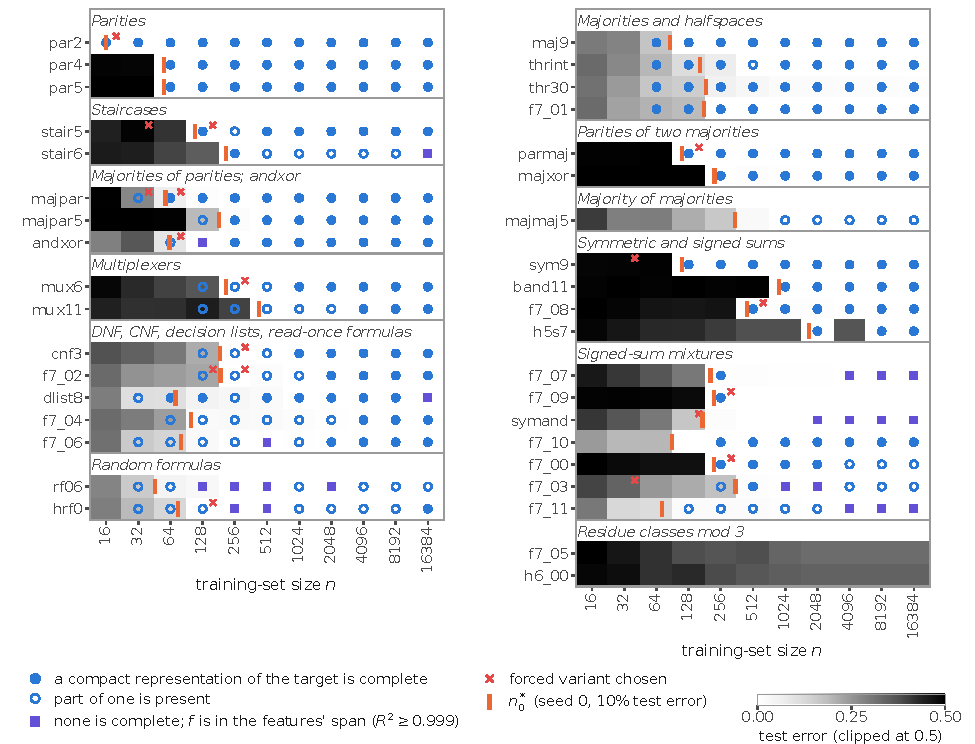
\includegraphics[width=\linewidth]{figures/fig_interp_atlas.pdf}
\caption{The structure atlas: DFG alone on 37 targets, seed 0, every grid $n$ \status{Numerical}. Grey: test error (white is 0). Markers: a compact representation of the target is complete in the model (filled dot; on a grey cell, the weights are not yet right), part of one is present (open dot), or none is complete but $f$ lies in the span of the model's features (square; held-out $R^2\ge0.999$). Cross: the cross-validation chose the forced variant. Bar: $n^*_0$, the seed-0 10\% test-error point. Families as in \cref{tab:interp-atlas}; suites in \cref{tab:interp-atlas-targets}. Re-plotted by \repo{paper_dfg/make_interp.py} from \repo{study/part11/interp/tables/atlas_cells.csv} and \texttt{atlas\_targets.csv}; the plotted values are in \repo{paper_dfg/tables/interp_numbers.json}.}
\label{fig:interp-atlas}
\end{figure}

\begin{table}[tbp]
\centering{\scriptsize\setlength{\tabcolsep}{2.6pt}\renewcommand{\arraystretch}{1.12}
\begin{tabularx}{\linewidth}{@{}>{\raggedright\arraybackslash}p{2.35cm}rr>{\raggedright\arraybackslash}Xcrr>{\raggedright\arraybackslash}X@{}}
\toprule
& \multicolumn{3}{c}{first $n$ with test error $\le0.1$} & complete & \multicolumn{3}{c}{$n=16384$}\\
\cmidrule(lr){2-4}\cmidrule(lr){6-8}
family (targets) & $n$ & error & what the model holds & first / 16384 & error & size & what the model holds\\
\midrule
Parities (par2, par4, par5) & 16--64 & 0 & $\chi_S$ alone & 3/3\,; 3/3 & 0 & 2 & $\chi_S$ alone\\
Staircases (stair5, stair6) & 128--256 & 0 & the prefix characters $x_1$, $x_1x_2$, \dots{} and one more Fourier character & 2/2\,; 1/2 & 0 & 17--81 & Fourier characters: all of stair5's; most of stair6's, and relevant blocks\\
Majorities of parities; andxor (majpar, majpar5, andxor) & 64--256 & 0.011--0.092 & their pair characters & 2/3\,; 3/3 & 0 & 4--29 & their characters; one relevant block in majpar and majpar5\\
Multiplexers (mux6, mux11) & 256--512 & 0--0.002 & characters and blocks on address and data bits & 0/2\,; 2/2 & 0 & 17--65 & exactly the Fourier expansion\\
DNF, CNF, decision lists, read-once formulas (cnf3, f7\_02, dlist8, f7\_04, f7\_06) & 128--256 & 0--0.049 & low-degree characters, blocks that encode a clause, term or rule, irrelevant degree-1 characters & 1/5\,; 4/5 & 0 & 67--181 & characters and a few blocks\\
Random formulas (rf06, hrf0) & 64--128 & 0--0.045 & the dominant input's character (hrf0: and a relevant block) & 0/2\,; 1/2 & 0 & 32--66 & Fourier characters (hrf0: its whole expansion)\\
Majorities and halfspaces (maj9, thrint, thr30, f7\_01) & 128--256 & 0--0.071 & degree-1 characters from the linear block; the exact block (maj9, f7\_01) & 4/4\,; 4/4 & 0--0.009 & 43--149 & degree-1 characters and a block\\
Parities of two majorities (parmaj, majxor) & 128--256 & 0--0.0005 & two folded blocks $|t_A+t_B|$, $|t_A-t_B|$ & 2/2\,; 2/2 & 0 & 19--137 & the cross-pair characters; majxor also both folded blocks\\
Majority of majorities (majmaj5) & 512 & 0.023 & 4-input pieces of a majority, modulated by its fifth input & 0/1\,; 0/1 & 0 & 256 & blocks and characters of odd degree 1--7: 256 features, DFG's cap\\
Symmetric and signed sums (sym9, band11, f7\_08, h5s7) & 128--2048 & 0--0.012 & the exact signed block (h5s7: two factors that partition its class) & 4/4\,; 4/4 & 0--0.0005 & 60--255 & the block, with relatives (sym9: and a spurious product)\\
Signed-sum mixtures (f7\_07, f7\_09, symand, f7\_10, f7\_00, f7\_03, f7\_11) & 128--512 & 0--0.016 & the partner's character, and the compact form or a relative of it & 4/7\,; 1/7 & 0 & 27--115 & weighted blocks with the partner as inner term, and characters\\
Residue classes mod 3 (f7\_05, h6\_00) & never & -- & never reached & 0/2\,; 0/2 & 0.3245--0.3430 & 1 & the constant and the kernel background, at every $n$\\
\bottomrule
\end{tabularx}
}
\caption{What DFG alone's model holds, family by family, seed 0 \status{Numerical}. ``First $n$'': the first grid $n$ at which the target's test error is at most 0.1; $n$ and the error are ranges over the family's targets. ``Complete'': the number of targets whose model holds some compact representation of the target completely, at that first $n$ and at $n=16384$. ``Size'': the number of features at $n=16384$, the constant included. The descriptions summarize \repo{study/part11/interp/ATLAS.md}, \S1; the numbers are computed by \repo{paper_dfg/make_interp.py} from \repo{study/part11/interp/tables/atlas_family.json} and \texttt{atlas\_cells.csv}. \Cref{tab:interp-atlas-targets} has every target.}
\label{tab:interp-atlas}
\end{table}

\Cref{fig:interp-atlas} shows every cell of the atlas and \cref{tab:interp-atlas} summarizes each family at its first fit (the first grid $n$ with test error at most 0.1) and at $n=16384$; \cref{app:interp-families} gives the models target by target.

\paragraph{Characters for juntas and formulas} \status{Numerical}. From the first fit on (par2 at $n=16$, par4 and par5 at 64), every parity's model is the constant plus the parity's character and nothing else, and staircases are their prefix characters. The first fits of the multiplexers and small formulas mix characters of degree 1--3 with blocks that encode an address, a clause, a term or a rule; the character representations are complete later. At $n=16384$, 8 of the 37 models are exactly the target's Fourier expansion: par2, par4, par5, stair5, andxor, mux6, mux11 and hrf0. \emph{Reading} \status{Heuristic}. For parities the dictionary is the target class, and the size at which DFG has the character is set by the union bound (\cref{prop:parity}). Characters enter in order of how detectable they are (\cref{sec:interp-when}); blocks encode a clause, term or branch before its characters are all detectable, and give way to them as they become detectable.

\paragraph{Blocks for sums, thresholds and mixtures} \status{Numerical}. Symmetric and signed-sum targets are their exact signed block (sym9 its folded block alone at $n=128$, with 4 features and error 0); what varies across them is not the form but when the search finds it (\cref{sec:interp-when,sec:interp-fail}). In the four analysed halfspaces the linear block enters at $n=64$ and makes the degree-1 representation complete, with oracle error at most 0.007, but DFG's own error is 0.17--0.20 until blocks arrive that encode the threshold (one block for maj9 and f7\_01, a product block for thrint); thr30, with Gaussian weights on all 30 inputs, is never fitted exactly (0.009 at 16384). A parity of two majorities is first fitted by two folded blocks over the union of their inputs, $|t_A+t_B|$ and $|t_A-t_B|$, which represent the target because $\mathrm{sign}(|t_A+t_B|^2-|t_A-t_B|^2)=\mathrm{sign}(t_At_B)$. In the seven signed-sum mixtures the partner's character comes first in 5 of the 6 that have one, and with more data the compact forms give way to weighted blocks with the partner as inner term: at $n=16384$ only f7\_10 still holds its compact form, though all seven have test error 0. \emph{Reading} \status{Heuristic}. For a threshold function the dictionary is complete almost at once, and the logistic readout of 30 noisy degree-1 coefficients learns the weights slowly where one block does it at once. DFG treats a partner variable as a heavy input of the block rather than as a modulator, because the partner is itself a strong single input or pair.

\paragraph{Dictionary or readout} \status{Numerical}. Of the 148 cells with test error above 0.1, the learned features cannot express the target (oracle error above 0.1) in 133. In 9 they can (oracle error at most 0.02), and only DFG's own weights fall short, all just after the linear block entered; the other 6 lie in between. The oracle leaves out the kernel background, so ``cannot express'' concerns the learned features only: in 27 of the 133 cells DFG's own error is more than 0.05 below the oracle's, because the background carries the signal there. At the first fit, DFG's error is within 0.0005 of the oracle's for the median target; the largest readout gap is thrint's at 256, 0.071, on a complete degree-1 dictionary. \emph{Reading} \status{Heuristic}. Outside threshold functions, DFG's data cost is the cost of getting the right features into the model; once they are in, its readout is close to the best weights for them.

\paragraph{Spurious terms, and v3's member} \status{Numerical}. At $n=16384$ the spurious share is at most 0.1 for 36 of the 37 targets, and removing the spurious terms leaves every test error unchanged (\cref{app:interp-spur}). Part 10's analysis of the same code as v3's member \cite{portfoliolearner2026} carries over: over the 255 seed-0 cells the two analyses share, the DFG test error is identical in 141, and most differences at small $n$ come from the stacker (\cref{app:interp-v3}).

% sections/interp_dyn.tex: part 2 of \cref{sec:interp} ("What it learns"), \input at the end of sections/interp.tex:
% the two regimes, the failures, false admissions and the order of acquisition.  Figures and tables come from
% make_interp.py; the numbers quoted here that no figure or table shows are stored in tables/interp_numbers.json, or
% come from the analysis reports and their outputs that the text names (THEORY.md, ORDER.md, CALIB.md, ABLATIONS.md).
% The full versions of these subsections are in sections/app_interp.tex.

% ======================================================================================================================
\subsection{Two regimes: when the structure appears, and when its test would admit it}\label{sec:interp-when}

Apart from the forced variant's guesses, each piece of a target's structure has two sizes: the training-set size from which DFG's test would admit it if the search offered it, and the size from which the model holds it. For characters the search offers every candidate of a class; for sum blocks it offers only blocks grown from statistics of one or two inputs (\cref{prop:blocks}), so the two sizes can be far apart. This subsection measures both and then moves the tests' threshold (detail in \cref{app:interp-when}).

\begin{figure}[tbp]
\centering
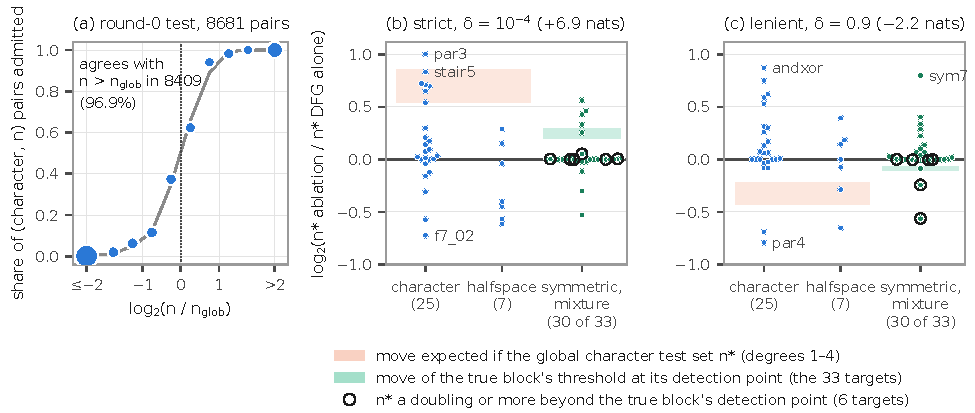
\includegraphics[width=\linewidth]{figures/fig_dyn_when.pdf}
\caption{The test and the data cost. (a)~DFG's round-0 decisions on the target characters of degree $\le4$ against the detection size $n_{\rm glob}$ (41 \code{designed} and \code{random} targets, seed 0, every grid size; 8681 (character, $n$) pairs) \status{Numerical}: the share admitted in each band of $\log_2(n/n_{\rm glob})$ (area $\propto\sqrt{\text{pairs}}$; end bands open), and a normal approximation for $v_S$ (line). (b, c)~\code{strict} and \code{lenient}: $\log_2(\nstar_{\rm ablation}/\nstar_{\rm DFG\ alone})$ per target (seeds 0 and 1, paired), by the ablation analysis's class; the three residue classes, which neither run learns, are not drawn \status{Numerical}. Orange: the move of $n_{\rm glob}$ for one character of degree 1--4, the move of $\nstar$ if a round-0 character test set it \status{Heuristic}. Green: the range of the true block's threshold move at its detection point over the 33 symmetric and mixture targets \status{Numerical}. Rings: the 6 targets whose $\nstar$ lies a doubling or more beyond that point (\cref{app:interp-when}). Sources: \repo{study/part11/interp/theory/check_theory.json} (\texttt{P3.test0}), \repo{study/part11/RESULTS.json} (\texttt{q5\_ablations}), \repo{study/part11/interp/ablations/ablations.json} and \repo{study/part10/interp/tables/toy_timing.csv}, via \repo{paper_dfg/make_interp.py}.}
\label{fig:dyn-when}
\end{figure}

\paragraph{Characters: admitted by detectability} \status{Proved, then Numerical}. In round 0 a character $\chi_S$ of degree $k$ searched on all rows passes its test exactly when $n>2c^2L_k\,s^2/v_S^2$ (\cref{prop:nglob}); replacing $v_S$ by the target's coefficient $\hat f(S)$ and $s^2$ by $1-\hat f(\emptyset)^2$ gives the \emph{detection size} $n_{\rm glob}(S)$ of \cref{eq:nglob}, a first-order prediction \status{Heuristic}. Degree enters only through the logarithm: with $K=4$, $\delta=0.1$ and $c=1$, $L_k$ is 8.5, 11.2, 13.4 and 15.3 nats for $k=1$--4 at $d=30$, so a coefficient $\sqrt{15.3/8.5}=1.34$ times larger at degree 4 than at degree 1 already has the smaller $n_{\rm glob}$. On the 41 targets of \code{designed} and \code{random}, DFG's round-0 decision agrees with ``admit when $n>n_{\rm glob}$'' in 8409 of 8681 (character, $n$) pairs (96.9\%; \cref{fig:dyn-when}a), and the 249 characters that first enter through this test do so at a median $2^{0.26}\,n_{\rm glob}$. The classes of later rounds admit characters a median 1.4 to 3.7 doublings below $n_{\rm glob}$, mainly because the residual there is 3.2 to 19 times smaller (class medians; \cref{tab:dyn-when}a): once the large terms are fitted, characters on the inputs already in use pass the tests of small classes, which resembles the junta completion that Part~5 saw in the networks \cite{gdcircuit2026} \status{Heuristic}. For a parity no search stands between the test and the model: \cref{prop:parity}'s criterion holds in all 250 parity cells with $n\ge32$.

\paragraph{Sum blocks: detection is cheap, discovery lags} \status{Numerical}. Part~10 measured both sizes for v3's DFG member on the 54 sum-structured targets \cite{portfoliolearner2026}: $n_{\rm detect}$, the first grid size at which DFG's block test would admit the target's \emph{true} block if it were proposed in round 0 (an oracle), and $n_{\rm struct}$, the first at which the model holds every signed-symmetry class of size $\ge3$ exactly. Over the 49 found, with the detection points that Part 10's verifier corrected for the gate and multiplexer mixtures, $n_{\rm struct}$ is earlier than $n_{\rm detect}$ for 6, equal for 20, one doubling later for 9 and two or more doublings later for 14, and the delay grows as the target's share of variance at Fourier degrees 1--2 shrinks (Spearman $-0.54$ over all 54). Part 10 labelled its reading, that the search sets the data cost, Heuristic: nothing isolated the search, and the stacker's choice between DFG's two variants could also have contributed. On the 13 sum-structured targets of the atlas DFG alone's $n_{\rm struct}$ equals that of v3's member (\cref{tab:dyn-when}b): the delay is 0 for 4, one doubling for 3, and two to six doublings for f7\_08, band11 and h5s7, and three never reach it. When the block enters, its statistic is well above the threshold (in Part~10's runs, a median 2.3 times at $n_{\rm struct}$ over the 22 pure symmetric targets found, range 0.89--74).

\paragraph{Moving the threshold} \status{Numerical, then Heuristic}. \code{strict} ($\delta=10^{-4}$) adds 6.9 nats to the log term of every test, and \code{lenient} ($\delta=0.9$) subtracts 2.2 (\cref{sec:ablations}; \repo{study/part11/interp/ablations/ABLATIONS.md}, post hoc, corrected after an independent verification). If a round-0 character test set $\nstar$, \code{strict} would raise it by $+0.54$ (degree 4) to $+0.86$ doublings (degree 1) \status{Heuristic}. The block test's log term is larger (33.7 nats for an unmodulated 11-input block), so at the true blocks' detection points \code{strict} moves its threshold by only $+0.20$ to $+0.30$ doublings of $n$ (re-thresholded post hoc; approximate for the modulated blocks, whose statistic was stored only as a ratio to its threshold). \Cref{fig:dyn-when}b,c shows what happened.
\begin{itemize}
\item \emph{Parities: the test sets the cost exactly.} \Cref{prop:parity} with $\delta$ moved, applied to each training set's own $\bar y$, predicts the measured changes to within 0.03 (par3 $+0.98$ against $+1.00$ under \code{strict}; par4 $-0.79$ against $-0.79$ under \code{lenient}).
\item \emph{Other character targets: one grid step where the test binds.} \code{strict} raises $\nstar$ by more than 0.25 on 8 of the 25, mostly by about the predicted amount. \code{lenient} is not the mirror image (2 lower, 8 higher): those targets are first fitted at small $n$, mostly by the forced variant, and with $\delta=0.9$ the linear block enters and the cross-validation's choice of variant changes (\cref{sec:abl-test}).
\item \emph{Halfspaces: a stricter test helps} ($-0.23$; $-0.17$ counting f7\_10): a degree-1 character that passes first takes part of the block's signal (\cref{app:interp-when}).
\item \emph{Symmetric and mixture targets: $\nstar$ stays} (class means $+0.04$ and $+0.05$; 30 of the 33 learned). On the 6 targets whose $\nstar$ lies a doubling or more beyond $n_{\rm detect}$ (band11, f7\_08, h6\_01, h6\_02, h6\_06, h6\_08; ringed in \cref{fig:dyn-when}), \code{strict} changes $\nstar$ by at most 0.05, although it moves their blocks' threshold by about a quarter of a doubling. These use the corrected detection points; with the uncorrected points, which the ablation analysis uses, there are 7 (f7\_03 as well, on which \code{strict} changes $\nstar$ by 0.00). On the other 24, $\nstar$ lies less than a doubling beyond $n_{\rm detect}$, and for 20 of them at or below it (23 and 18 with the uncorrected points), so the grid cannot separate the test from the search.
\end{itemize}
\emph{Reading} \status{Heuristic}. Where $\nstar$ lies a doubling or more beyond $n_{\rm detect}$, a test about a quarter of a doubling stricter changes nothing, because once the search proposes the block, the test admits it well above its threshold: \emph{there the search, not the test, sets the data cost}; on the other sum targets the grid cannot tell the two apart. Where the first fit comes from a character test, the test binds and $\nstar$ moves with the threshold: exactly for the parities, within a grid step for the staircases and small formulas. Where the first fit comes from the forced variant, $\delta$ acts through the linear block and the cross-validation instead, and the sign of its effect does not follow from the test. Part~10's reading rested on correlations; the ablations add an intervention on the test. They still do not isolate the search, for example by seeding it with the true block, and they say nothing about the residue classes, which neither run learns.

% ======================================================================================================================
\subsection{Where it fails, and why}\label{sec:interp-fail}

\paragraph{The residue classes mod 3: detectable, but out of the search's reach.} f7\_05, h6\_00 and fd\_10, residue classes mod 3 of signed counts of 14, 13 and 10 inputs (\cref{tab:interp-mod3}), are three of the four sum-structured targets that DFG alone never learns, and v3 does not learn them either: DFG's model is the constant plus the kernel background at every $n$.
\begin{itemize}
\item \emph{The test would accept the block.} One block, with one group per value of its signed sum, represents each target with at most $k+1$ parameters, where the target's Fourier expansion has all $2^k-1$ non-constant characters \status{Proved}. DFG's grouping merges the rarest values, which costs 0.1--0.2\% error, and Part 10 found the true block passing DFG's test from $n=128$ on the same training rows, at 134--155 times the threshold at $n=16384$ \status{Numerical}.
\item \emph{The search's seeds see nothing.} The targets' Fourier weight at degrees 1 and 2 is exactly $1.6\cdot10^{-6}$, $5.4\cdot10^{-6}$ and $2.1\cdot10^{-4}$, and every starting point of the block search is computed from statistics of one or two inputs, whose expectations in round 0 are the target's degree-1 and degree-2 coefficients \status{Proved, \cref{prop:blocks}(f)}: here $2^{-13}$, $2^{-12}$ and $2^{-9}$ in absolute value \status{Numerical, exact}. By the BBP threshold for a rank-one perturbation of a random matrix \cite{baik2005phase,benaychgeorges2011eigenvalues}, the top eigenvector of the residual pair matrix would point at the block only from $n\approx1.1\cdot10^7$, $3.1\cdot10^6$ and $8.6\cdot10^4$ \status{Heuristic}.
\item \emph{Exhaustive search does not help within the budget.} Part 10 counted $1.5\cdot10^{10}$ to $1.2\cdot10^{12}$ blocks of the true size, each costing at least $n$ operations to score, against $1.62\cdot10^{11}$ FLOPs per fit \cite{portfoliolearner2026} \status{Numerical}.
\end{itemize}
\begin{table}[tbp]
\centering{\footnotesize\setlength{\tabcolsep}{2.6pt}
\begin{tabular}{@{}llrrrrrrrr@{}}
\toprule
& & & & & \multicolumn{2}{c}{true block: test} & \multicolumn{2}{c}{search's seeds} & DFG alone\\
\cmidrule(lr){6-7}\cmidrule(lr){8-9}
target & definition & $k$ & $W_1+W_2$ & peak & passes from & \hd{over threshold\\at 16384} & \hd{signal/noise\\at 16384} & \hd{eigenvector\\needs $n$} & \hd{error at\\16384}\\
\midrule
f7\_05 & $[B\bmod3 \ne 0]$ & 14 & $1.6\cdot10^{-6}$ & 11 & 128 & 134 & 0.017 & $1.1\cdot10^{7}$ & 0.3245\\
h6\_00 & $[B\bmod3 \ne 1]$ & 13 & $5.4\cdot10^{-6}$ & 9 & 128 & 139 & 0.033 & $3.1\cdot10^{6}$ & 0.3430\\
fd\_10 & $[B\bmod3 = 0]$ & 10 & $2.1\cdot10^{-4}$ & 7 & 128 & 155 & 0.265 & $8.6\cdot10^{4}$ & 0.3240\\
\bottomrule
\end{tabular}
}
\caption{The three residue classes mod 3 \status{Numerical, Heuristic}. $B$: the block's $k$ signed inputs that equal $+1$. $W_1+W_2$: the exact Fourier weight at degrees 1 and 2 \status{Numerical: exact rationals from the formula of \cref{prop:blocks}(d), which is Proved}; ``peak'': the degree with the most weight. True block: the first grid $n$ at which its test passes on the seed-0 rows, and its statistic over the threshold at $n=16384$ (Part~10, same code) \status{Numerical}. Search's seeds: the signal-to-noise ratio of one pair-matrix entry inside the block at $n=16384$, and the $n$ from which the top eigenvector would point at the block \status{Heuristic}. DFG alone: the test error at $n=16384$, equal in its three seeds to the minority rate. Sources: \repo{study/part11/interp/theory/check_theory.json} (\texttt{P4.targets}), \repo{study/part10/interp/results/toy_final/power/} and the Part 11 result files, via \repo{paper_dfg/make_interp.py}.}
\label{tab:interp-mod3}
\end{table}

\emph{Reading} \status{Heuristic}. A residue class mod 3 is detectable once proposed and invisible from every foothold the search has; more data within any practical range would not help the seeds. Only the most regularized network, \code{nets_cewd1.0}, learns h6\_00 ($\nstar=12304$), the one sum-structured target on which a network beats DFG alone; how it gets there was not analysed.

\paragraph{h5s1, and arbitrary accept sets} \status{Numerical, then Heuristic}. h5s1, an arbitrary accept set of a signed 9-input sum times the parity $x_{10}x_{11}$, is learned by no learner. Its modulated block would pass DFG's test from $n=128$, but DFG builds a modulated block only on a character already in the model, and the pair's coefficient is exactly $-1/32$, so its round-0 test admits it in expectation only from $n_{\rm glob}=2.3\cdot10^4$, above the grid \status{Heuristic}. The six signed-sum targets that DFG learns last are all pure arbitrary accept sets ($\nstar$ from 597 to 6186, against a median of 186 over the 50 sum-structured targets it learns), whose share of variance at Fourier degrees 1--2 is 0.008--0.081, against a median of 0.34 over the 54 (\cref{app:interp-fail}, with h5s7's dependence on the training set).

% ======================================================================================================================
\subsection{False admissions}\label{sec:interp-calib}

How often does DFG admit a feature when there is nothing to find? The analysis fits DFG alone on labels drawn independently of the inputs, balanced ($P(y{=}1)=0.5$) or biased (0.8), at $d=30$ and 60 and every $n$, and computes each test's null pass rate (\repo{study/part11/interp/calib/CALIB.md}, with the corrections of \repo{study/part11/interp/calib/VERIFY_CALIB.md}; \cref{tab:interp-calib} in \cref{app:interp-calib}).
\begin{itemize}
\item \emph{The character tests sit about ten times inside their bound} \status{Proved, then Numerical}. \Cref{prop:null} bounds a false character of degree $k$ in round 0 by $\delta/(2K)=0.0125$, for any $d$ and $n$. In the final fits on noise the global classes passed in 2 of 2400 class searches at $d=30$ and 1 of 840 at $d=60$, and the null rate is about 0.1\% per test. The bound exceeds the independent-Gaussian rate by 10.9--14.3 at $d=30$, close to the Mills-ratio factor, so Hoeffding's inequality is what is loose \status{Heuristic}. On balanced labels none of the 220 final models at $d=30$ holds a feature that passed a test (95\% upper limit 0.017), and 5 of 110 at $d=60$ do.
\item \emph{The linear block} passes at about 1\%, a tenth of its nominal $\delta=0.1$, but each false pass adds all $d$ inputs (test error 0.336 and 0.283 against 0.195 for a constant prediction, in the two cases on biased labels at $d=30$).
\item \emph{The spectral block has no proved level.} On balanced labels it passed in at most 3 of 20\,000 null draws, but on biased labels at $n=4d$, the smallest $n$ at which it runs, in 5.4\% at $d=30$, 47\% at $d=60$ and 99\% at $d=120$ ($P(y{=}1)=0.8$), and 39\% at $d=30$ with $P(y{=}1)=0.9$.
\item \emph{The sum blocks have no proved level either.} They never passed in the 660 final fits on noise, but they did in round 0 of 2 fold fits at $d=30$ with $P(y{=}1)=0.8$, and in 1 of THEORY.md's 30 fits at $P(y{=}1)=0.85$.
\item \emph{The forced variant is not calibrated after its guesses}: after two forced characters the local class can admit their product, as in 229 of 900 forced fold fits on biased noise at $d=30$, but the paired cross-validation chose the forced variant in none of the 180 biased final fits.
\item \emph{Spurious terms} on the \code{designed} and \code{random} targets are mostly the linear block's (961 of the 1047 terms that read an irrelevant input), and from $n=128$ on removing them changes the mean test error by at most 0.0002; on noise the kernel background, not the features, costs error, up to 0.144 (\cref{app:interp-spur,app:interp-calib}).
\end{itemize}

% ======================================================================================================================
\subsection{The order of acquisition, against the Part 5 networks}\label{sec:interp-order}

Part~5 traced the order in which small ReLU networks acquire the Fourier characters of 11 \code{designed} targets at $d=30$ \cite{gdcircuit2026}: a linear stage first, bundles of characters carried by one new hidden-unit direction, an order that follows how the target is built (low degree first, products of learned features after their factors) more than coefficient size, and later stages that stop partway at finite $n$. The order analysis compares DFG alone's order with the networks' on the same targets and training sets, in 363 fits (\repo{study/part11/interp/order/ORDER.md}, corrected after an independent verification). A character's \emph{learned fraction} $\varphi_S$ is the model's coefficient on $\chi_S$ over $\hat f(S)$. The networks' \emph{time order} ranks characters by the training step at which the seed-mean $\varphi_S$ first reaches $1/2$ and stays above 0.4, in Part 5's online runs (trained on a fresh sample at every step), and their \emph{$n$ order} by the smallest grid size from which $\varphi_S\ge1/2$ after 20000 steps, with $\varphi_S\ge0.4$ at every larger $n$. DFG has a \emph{round order}, a \emph{round-0 priority} (the order of round-0 $z$-scores) and an \emph{$n$ order} by the networks' rule; only the two $n$ orders are like for like (\cref{app:interp-order}).

\paragraph{What agrees} \status{Numerical}. At Part 5's sample sizes, $n=512$, 2048 and 16384, DFG admits every target character it will ever carry in a single round in 24, 30 and 32 of the 33 fits, so its round axis is empty where the networks' time axis is richest; at small $n$ its round order agrees moderately with the networks' time order (mean Kendall $\tau$ 0.44 at $n=64$ and 128). Inside round 0 the priority is positively rank-correlated with the networks' order on all 11 targets in each of four conditions (at $n=16384$ from 0.22 to 0.81, median 0.54). On the $n$ axis the agreement is moderate (median $\tau$ 0.40 against both of the networks' orders), while the networks' two orders agree with each other at median 0.75.

\paragraph{The networks follow construction, DFG follows detectability} \status{Numerical, then Heuristic}. On the 8 targets whose coefficient sizes differ, the networks' time order follows degree more than coefficient size on 7, and DFG's $n$ order follows $1/|\hat f(S)|$ more than degree on 5. Mux is the clearest case: its largest term $x_1x_2x_3x_4$ ($\hat f(S)=0.75$, degree 4) is the networks' last character (online at 452 steps, against 60--66 for the linear terms) and DFG's first by round-0 priority, in all 27 fits with $n\ge64$; its $n_{\rm glob}$ is 54, against 271 for the linear terms. For the 64 characters of degree $\le4$ with $|\hat f(S)|\ge0.25$, DFG's median $n$ onset is 4 times smaller than the networks' (median $\log_2$ ratio $-2.0$). \emph{Reading} \status{Heuristic}. For DFG a character costs data roughly logarithmically in its degree and quadratically in $1/\hat f(S)$; Part~5's model of the networks charges training time as $e^2$ in the number $e$ of new inputs a move coordinates, and only as $\rho^{-1/2}$ in its share $\rho$ of the residual. The orders therefore agree where a target's large coefficients sit at low degree (sparsepoly, majpar, rmaj9: $\tau=0.68$--0.71 against the time order), invert where a large coefficient sits at high degree (mux), and disagree where a stage mixes sizes (stair5, dnf3, rand3). \emph{Caveats.} Three seeds, one network architecture and $d=30$ only; the 11 targets come from a few designed families, so no $p$-values are quoted; DFG's $\varphi$ is that of its least-squares function, and the logistic refit can distort single coefficients.


\section{Discussion}\label{sec:discussion}

\subsection{What kind of learner DFG turned out to be}\label{sec:disc-kind}

\paragraph{An Occam learner over a Boolean dictionary, made greedy by a residual} \status{Heuristic, from \cref{sec:learner,sec:guarantees}}. DFG's character test admits a feature when the residual sum of squares it would remove exceeds the code length of naming it in its class, $2c^2\ln(4KN/\delta)$ in units of the residual's variance (\cref{sec:relates}), so a character passes, to first order, once $n$ exceeds its detection size, in which its degree enters only through the logarithm and its coefficient through its inverse square (\cref{prop:nglob}). The candidates come from the low-degree algorithm's enumeration and from a heuristic search for signed-sum blocks seeded by the residual's degree-1 and degree-2 statistics. The residual makes the loop greedy: each round's tests are calibrated to the noise left by the previous round, so weaker features pass once stronger ones are fitted (\cref{sec:abl-label}).

\paragraph{Two regimes} (\cref{sec:interp-when}). \emph{Test-limited} \status{Proved, Numerical; Heuristic beyond the parities}: where the structure lies in an enumerated class, the search offers every candidate, and for parities the union bound sets the first fit exactly. \emph{Search-limited} \status{Numerical, then Heuristic}: where the structure is a signed-sum block, the test would often admit the true block well before the model holds it, and where the grid can tell, the data cost is set by when the block search first proposes the block, the later the less of the target's variance sits at Fourier degrees 1--2; the residue classes mod 3 give the search no foothold at all. Halfspaces sit between the two: the dictionary is complete at $n=64$, but DFG's weights on it are poor until blocks that encode the threshold enter, and thr30 is never fitted exactly.

\paragraph{Its relation to the networks' greedy feature growth} \status{Heuristic}. DFG kept the loop of the picture it was built from and replaced the search (\cref{sec:relates}). What survived is the loop: residual-driven growth, later rounds that make a junta's remaining characters cheaper, and a Hebbian background. What changed is the price of a feature, and with it the order in which features come (\cref{sec:disc-gd}).

\subsection{Why it needs less data than the networks here}\label{sec:disc-why}

\paragraph{The logarithm of the dictionary against a power of $d$.} For a $k$-parity DFG's round-0 test passes $\chi_S$ exactly when $n(1-\bar y^2)>n_{\rm thr}(k,d)$, which grows like $2k\ln d$ \status{Proved; \cref{prop:parity}}, and DFG's $\nstar$ on the parities moves by at most one grid step over $d=15$--120 \status{Numerical; \cref{fig:dscale}}, while the networks' $\nstar$ grows about like $d^{k-1}$ for $k\le3$ \status{Numerical; \cref{tab:dscale}}, the rate of the leap and correlational-SQ analysis \cite{abbe2023leap}; more generally, SGD learns $k$-sparse parities in $d^{O(k)}$ steps, near the statistical-query limit \cite{barak2022hidden}. Part 3's model of the networks explains the gap \cite{gdcircuit2026}: a move that needs $k$ new inputs and has correlation $\rho$ with the residual is accepted once $n\rho^2\gtrsim2.25\,d\max(1,d/18)^{k-2}$, with the two constants fitted to the networks, about $d^{k-1}$: the noise level of a continuous search over directions, not the best-of-$N$ level of a union bound, which DFG's test is, $n\rho^2\gtrsim2\ln(4KN/\delta)$ (\cref{prop:nglob}) \status{Heuristic}. With a noise-free search, that model's $\nstar$ fell to 16--87 on every target, as far from the networks as an Occam learner. In those terms DFG is the networks' greedy loop with the search's sampling noise removed and paid for in enumeration.

\paragraph{Enumeration pays in FLOPs, not samples} \status{Proved, by the code; Numerical}. An exhaustive degree-$k$ search costs about $n\binom dk$ FLOPs times a constant (\cref{prop:compute}), while one network run costs FLOPs linear in $d$, so DFG's budget subsamples the search, and at $n>512$ the budgeted global search can pass no degree-4 character from $d=179$ on, and no degree-3 character from $d=630$ on, because its rows fall below the floor of \cref{prop:floor} (\cref{app:proof-parity}). Beyond that point a degree-4 parity with no lower-degree footprint is found only by the block search's chance hits, as in the \code{K3} and core runs. So within one network run of compute, DFG's Occam rate on degree-4 structure holds up to $d$ of about 120--180; further out it needs more compute than the networks use, unless a search replaces the enumeration \status{Heuristic}.

\paragraph{Signed sums: the same foothold, rounded and tested} \status{Heuristic}. DFG's block search starts from the residual's degree-1 and degree-2 statistics (\cref{prop:blocks}(f)), the statistics a network's early gradient also sees, whose top eigenvector gives the support and the signs of a block (\cref{sec:round}). DFG needs fewer samples because it rounds a coarse estimate of that direction to an exact signed subset and then tests the whole block under one union bound, while a network has to learn the direction to useful precision by noisy local steps, as in the information-exponent picture of single-index learning \cite{benarous2021online,damian2024gaps}. On the five sum-structured \code{dlheld7} wins DFG needs about $4.3\times$ less data than the best network variant; on the other five, where a no-search baseline also beats them, the networks are slow and DFG's search earns little (\cref{sec:res-dlheld7}) \status{Numerical}.

\subsection{Its failures, in summary}\label{sec:disc-fail}

\paragraph{No low-degree foothold} \status{Proved, Numerical, Heuristic as marked}. The residue classes mod 3 put almost no Fourier weight at degrees 1--2 \status{Proved; \cref{prop:blocks}(e)}, where every starting point of the block search looks, although one block represents each of them and passes DFG's test from $n=128$ \status{Numerical}; the eigenvector seed would point at the block only from $8.6\cdot10^4$ to $1.1\cdot10^7$ rows \status{Heuristic; \cref{sec:interp-fail}}, and an exhaustive search over blocks of their size does not fit in the budget. The limit is shared: no learner in the study learns f7\_05, and only the most regularized network learns h6\_00. h5s1 is a milder case: its modulator's test passes in expectation only above the grid.

\paragraph{Small $n$} \status{Numerical, then Heuristic}. DFG's weakest range is $n\le128$, before its tests admit features; there v3's other members (trees, nearest neighbours, logistic regression) carry the fit on most of the 42 targets where DFG alone needs clearly more data than v3 (\cref{sec:res-v3}). DFG's own small-$n$ machinery is conservative: its paired cross-validation keeps the forced variant's right guesses less often than a stacker does, and its kernel background costs data on balance on the ablation suites (\cref{sec:abl-smalln}). This is the one place where the portfolio around DFG added something on Boolean targets.

\paragraph{Dense real-valued signal} \status{Numerical, then Heuristic}. DFG v1.3 does not run on real-valued data, and Part 7's three adaptations of DFG v1.1 were about level with a plain MLP on held-out tabular data, behind an L2-regularized one, and worse than a plain MLP on MNIST and Fashion-MNIST in 7 of 14 cells each \cite{discretelearners2026} (\cref{app:tabular}). Part 7's reading was that the useful features of dense real-valued signal are not in any small enumerable dictionary, and that union-bound tests stop growth early on many weak, correlated effects. The Boolean results contain a small echo: thr30, a halfspace with Gaussian weights on all 30 inputs, is never fitted exactly (test error 0.009 at $n=16384$).

\paragraph{Calibration at larger $d$} \status{Numerical}. The spectral test's null pass rate on biased labels near $n=4d$ grows with $d$ (\cref{sec:interp-calib}), so at larger $d$, or on strongly biased targets, DFG can be expected to admit more spurious spectral features \status{Heuristic}.

\subsection{DFG as a model of gradient descent}\label{sec:disc-gd}

\paragraph{What the order comparison supports} \status{Numerical} (\cref{sec:interp-order}). Inside one round the priorities agree, moderately, on all 11 targets in all four conditions, and at small $n$ the round order agrees moderately too; both loops make the rest of a junta cheaper once its first characters are in, and both carry a linear, Hebbian component.

\paragraph{What it does not support} \status{Numerical, then Heuristic}. Not a correspondence of time: at Part 5's sample sizes DFG's rounds collapse into one. Not the same price of a feature: the orders invert where a large coefficient sits at high degree. Not a linear stage: on all 8 targets with linear terms the networks learn every linear term before any other, while in DFG's $n$ order the linear terms come strictly first in only 6 of the 24 target-seed cases (\cref{app:interp-order}). And not the same sample complexity, $d^{k-1}$ against $\ln d$ on parities, so DFG is not a model of how much data gradient descent needs; the race model of Parts 2--3, a discrete model with a noise-limited feature search, is such a model, which matched the networks' sample sizes within a factor of about 1.3 on held-out functions \cite{gdcircuit2026}. \emph{Reading} \status{Heuristic}. DFG models the outcome of greedy feature growth, the features a greedy residual loop ends with, at one extreme of the trade between data and compute that networks also make \cite{edelman2023pareto}. It does not model the dynamics. The two orders agree where a target's large coefficients sit at low degree, so that detectability and construction coincide, and they come apart where they do not.

\subsection{The core DFG as the object to study next}\label{sec:disc-core}

\emph{Everything here is post hoc.} The core of \cref{sec:core} is level with DFG on average at a tenth of its FLOPs, though it moves many targets in both directions, and its largest losses are where a removed part has no substitute.

\paragraph{Why it is the better object} \status{Heuristic}. Every test in the core is a union bound over an explicit class, its heuristics are the block search and the small-$n$ forced guess with its cross-validated choice, and its readout is plain least squares, with no logistic refinement, spectral directions or background. The questions it poses are therefore sharper than DFG's:
\begin{itemize}
\item \emph{When does the block search find a block?} The BBP argument for the eigenvector seed is heuristic, and the core does not even use that seed: it grows blocks from the strongest pairs and single inputs. A statement of the form ``a function of a $k$-input signed sum with low-degree weight $W_1+W_2\ge w$ is proposed from $n\ge f(k,d,w)$'' would turn the search-limited regime into a sample bound.
\item \emph{Does the block test hold its level?} Its groups are a data-dependent partition of the rows, so the Gaussian calibration of \cref{eq:blocktest} is not proved; on noise it never passed in a final fit, but it did in fold fits on biased labels.
\item \emph{What does the forced variant buy?} Its guesses are the first fit of 12 of the 37 atlas targets (\cref{app:interp-fits}), and the paired test that chooses it is conservative; a calibrated replacement would make the small-$n$ behaviour analysable.
\end{itemize}
The core was defined after every result had been read, \code{dlheld7}'s included, so any claim about it beyond a description needs fresh data.

\subsection{What would test it further}\label{sec:disc-next}

\begin{enumerate}
\item \emph{Fresh suites from other families}, written independently of both the blind family and DFG's dictionary (higher-degree sparse polynomials, intersections of several halfspaces, interacting sums, residues mod $q$), since the held-out evidence is one draw of 12 targets from one generator whose design was known.
\item \emph{Larger $d$ with the networks}: degree-3 and degree-4 structure at $d=60$--250, where the budget first subsamples and then skips the degree-4 search.
\item \emph{The core, pre-registered,} on fresh suites that include the kinds of target it is predicted to lose.
\item \emph{Real-valued data with dictionaries derived from the data}: the residual loop and the union-bound test over classes of thresholds, quantile bits or residual-derived directions, with their sizes counted honestly, against gradient boosting, regularized MLPs and Part 7's adaptations.
\item \emph{Theory for the search}: a success probability for the block search as a function of the low-degree weights and $n$, levels for the block and spectral tests, and a bound on the test error of the fitted model, which none of \cref{sec:guarantees}'s statements gives.
\item \emph{Stronger references}: networks tuned per target, more seeds, and CPU time measured under a controlled load.
\end{enumerate}

\subsection{Limits}\label{sec:disc-limits}

\begin{itemize}
\item \textbf{The held-out set is small.} \code{dlheld7} has 12 targets from one family and one draw, and on 5 of DFG's 10 wins there a no-search baseline, logistic regression or default gradient boosting, also beats the networks. Its standard error of 0.27 treats the targets as independent draws from the family.
\item \textbf{The other suites are in-sample} (\cref{tab:status}). Pooled numbers summarize the record, not held-out estimates; the margin against \code{nets_wd} is smallest on the three suites held out for some version of DFG, as selection on the others would produce, though the suites also differ in kind (\cref{sec:res-suites}).
\item \textbf{The references are untuned.} One architecture, width, learning rate and step count per variant, not tuned per target; \code{nets_best} is a hindsight minimum over 2 to 5 such variants, which favours the networks; and the $d$-scaling uses \code{nets}, the weakest variant at $d=30$ (\cref{sec:refs,sec:res-dscale}). Stronger networks would plausibly narrow the margins.
\item \textbf{One input law and one domain.} Uniform $\pm1$ inputs, mostly at $d=30$, and two tabular datasets whose 9 cells resolve little. Nothing here is about real-valued data or images.
\item \textbf{Seeds and noise.} $\nstar$ comes from test errors averaged over 2 or 3 training sets, with no confidence interval; the $\pm0.25$ band is a convention, not a significance test, and is smaller than the spread between single seeds; the ablations use one or two seeds, the core two, and most analyses seed 0 (\cref{sec:metrics}).
\item \textbf{Post-hoc analyses.} The core, the paired null, the target families, the leave-one-in runs and the refits were defined after the pre-registered results had been read, and ``removable'' is a reading of counts against one replicate of the paired null, with no significance level (\cref{sec:ablations}); the analyses were checked by independent verifiers, whose corrections are applied (\cref{app:provenance}).
\item \textbf{Descriptive interpretability.} Most analyses use seed 0, one training set per target and $n$. Their readings are labelled Heuristic, and the ablations, one part at a time, are the only interventions (\cref{sec:interp}).
\item \textbf{Compute.} FLOPs are DFG's own count, prediction is not charged, and CPU times were measured on a shared machine (\cref{app:compute}).
\item \textbf{AI-written.} The code, the runs, the analyses and this paper were produced and checked by AI agents (Claude), with independent AI verifiers for the analyses. No human has reviewed any of it (\cref{app:provenance}).
\end{itemize}


\bibliographystyle{plainnat}
\bibliography{refs}

\appendix
\section{Names used in this paper}\label{app:names}

\Cref{tab:names} lists the names of learners, parts of DFG, references, sets, targets and metrics that the paper uses. DFG v1.3 is \repo{study/part10/hyb_portfolio3/dfg13.py}, every toy target is defined in \repo{study/boolfuncs.py}, and the blind family in \repo{study/part9/heldout6/FAMILY.md}.

\begin{table}[p]
\centering\scriptsize\setlength{\tabcolsep}{4pt}\renewcommand{\arraystretch}{1.0}
\begin{tabularx}{\linewidth}{>{\raggedright\arraybackslash}p{3.45cm}>{\raggedright\arraybackslash}X}
\toprule
name & meaning\\
\midrule
\multicolumn{2}{l}{\emph{Learners}}\\
DFG; v1, v1.1, v1.2, v1.3 & discrete feature growth (\cref{sec:learner}): v1 and v1.1 (Part 6), v1.2 with sum blocks (Part 9), v1.3 with weighted blocks, forced blocks and a beam search (Part 10)\\
DFG alone, \code{dfg13-perm} & this paper's object: the frozen DFG v1.3 run by itself, inputs permuted per fit (\cref{sec:part11})\\
v1, v2, v3; \code{dfg}, \code{dfg_forced} & the portfolios of Parts 8, 9, 10 (\code{hyb_portfolio}, \code{hyb_portfolio2}, \code{hyb_portfolio3}); they stack DFG v1.1, v1.2, v1.3, as the two members \code{dfg} and \code{dfg_forced}, with classical learners\\
\code{p9_sum}, \code{p10_sum} & the Part 9 and Part 10 toy builders' candidates: v2's and v3's code on toy inputs\\
\code{lowdeg} & the thresholded low-degree algorithm: DFG's degree-$\le4$ characters without its search (\cref{sec:refs})\\
ablation tags & DFG alone with one constructor argument changed (\cref{sec:ablations}): \code{nosums}, \code{strict}, \code{lenient}, \code{noeig}, \code{noblocks}, \code{nocomp}, \code{noweighted}, \code{nosmalln}, \code{nobg}, \code{lsread}, \code{K3}, \code{labelnoise}\\
\code{dfg_bits}, \code{dfg_dirs}, \code{dfg_gates} & Part 7's three adaptations of DFG to real-valued data: bit characters, data-derived directions, threshold gates\\
\addlinespace
\multicolumn{2}{l}{\emph{DFG's search} (\cref{sec:learner})}\\
character $\chi_S$; degree & $\chi_S(x)=\prod_{i\in S}x_i$; $|S|$\\
residual $r$; $s$ & $r=y-{}$the least-squares fit on the current features; $s=\mathrm{rms}(r)$\\
round & a pass that searches every class on $r$, admits what passes its test and refits; at most 8\\
class; union bound $N$ & candidates enumerated and tested together; their number $N$ enters the threshold as $\ln(4KN/\delta)$, with $K=4$, $\delta=0.1$\\
global, extension, local class & every character of one degree $\le K$ on all $d$ inputs (5--6 on a subsample); $S\cup\{j\}$ and $S\cup\{j,l\}$ for admitted $S$; every subset of the $\le12$ inputs in use\\
linear block & all remaining degree-1 characters at once, admitted by a $\chi^2$ test on their coefficients\\
spectral feature & $(u\cdot x)^2-|u|^2$ for an eigenvector $u$ of the residual pair matrix $\frac1n\sum_tr_tx_tx_t^\top$ (diagonal removed) above its noise edge\\
sum block; statistic $t$ & signs $s_i\in\{\pm1\}$ on a subset $S$, and $t=\sum_{i\in S}s_ix_i$; the block's features are indicators of groups of values of $t$\\
folded, modulated, product block & $|t|$ in place of $t$; the indicators times an admitted character $\chi_T$; the joint cells of two blocks on disjoint supports\\
split, weighted block & a mixed-sign block as the product of its $+$ and $-$ parts; $u=t+a\tau$, $a\in\{\pm2,\pm3\}$, $\tau$ a literal, a 2-parity or an AND of two literals\\
block search & how blocks are proposed: from the residual's degree-1 and pair statistics\\
forced variant & at $n\le512$, takes the best candidate when nothing passes; kept only if it wins a paired cross-validation test\\
kernel background & one Hebbian step on the final residual, $\sum_ig_ix_i$ with $g_i=\frac1n\sum_tr_tx_{t,i}$, added to the output\\
readout & least squares on the admitted features, refined by 15 logistic Newton steps when $n\ge8p$\\
\addlinespace
\multicolumn{2}{l}{\emph{References} (\cref{sec:refs})}\\
\code{nets}, \code{nets_wd}, \code{nets_cewd}, \code{nets_cewd0.3}, \code{nets_cewd1.0} & the toy networks: square loss; square loss with weight decay 0.1; logistic loss with weight decay 0.1, 0.3, 1.0\\
\code{nets_best} & per target, the network variant with the smallest $\nstar$ among those run on its suite (hindsight)\\
\code{lin}, \code{hgb} & calibration references: cross-validated logistic regression on the inputs; default histogram gradient boosting\\
\code{mlp}, \code{mlp_reg}, \code{mlp_strong} & the baseline MLP (256-256); the same with an L2 penalty; an ensemble of three regularized MLPs\\
\code{mlp_best}, \code{mlp_best+} & per cell, the best of the MLP variants run there (hindsight); \code{mlp_best+} adds Part 9's wider ensembles\\
\addlinespace
\multicolumn{2}{l}{\emph{Sets and targets} (\cref{sec:tasks,tab:status})}\\
\code{designed}, \code{random}, \code{dlheld}--\code{dlheld7}, \code{dlsymdev}, \code{dlfamdev} & the 11 toy suites, at $d=30$ (\code{dlheld} is the first held-out suite); \code{designed} at $d=15,60,120$: the 7, 7 and 4 targets of Q4\\
the blind family & the random generator of \code{dlheld6}, \code{dlfamdev} and \code{dlheld7}, written blind to the sum-block design\\
sum-structured target & one of the 54 targets of \code{dlsymdev}, \code{dlheld4}--\code{dlheld7} and \code{dlfamdev} other than their 14 non-symmetric controls\\
accept set & the values of a sum on which a target, or a function of the sum in it, is $+1$\\
kr\_vs\_kp, mushroom & the two PMLB datasets with only binary or categorical columns and two classes\\
target names & f7\_, h6\_, fd\_: \code{dlheld7}, \code{dlheld6}, \code{dlfamdev}; h5s, h5t, h5rf: \code{dlheld5}; rf, rand, hrf, h2rf--h4rf: random formulas. Others are descriptive: par$k$ ($k$-bit parity), maj$k$, thr$k$ (halfspace), stair$k$, mux, dnf, cnf, dlist, sym, band, tail, \dots\\
development, exposed, held out & the statuses of a set for DFG v1.3 (\cref{tab:status})\\
\addlinespace
\multicolumn{2}{l}{\emph{Metrics} (\cref{sec:metrics})}\\
$\nstar$ & the training-set size at which the seed-mean test error reaches 10\%\\
$\log_2$ ratio; clearly better, worse & $\log_2(\nstar_A/\nstar_B)$; below $-0.25$, above $+0.25$, or only one of the two learners reaches 10\% error\\
suite mean; pooled & the mean ratio over the targets both learn; per-target ratios pooled over suites\\
cell; better, tie, worse & a (dataset, $n$) pair on tabular data; the verdicts of the cell rule\\
budget & one toy network run in FLOPs ($1.62\times10^{11}$ at $d=30$); for real data, three training runs of \code{mlp}\\
$n_{\rm glob}$ & where a character passes round 0's global test in expectation: $2\ln\bigl(4K\binom d{|S|}/\delta\bigr)\bigl(1-\hat f(\emptyset)^2\bigr)/\hat f(S)^2$ (\cref{sec:interp})\\
$n_{\rm detect}$ & the first $n$ at which DFG's own test would admit the target's true block if the search proposed it (\cref{sec:interp})\\
$n_{\rm struct}$ & the first analysed $n$ at which DFG's model holds the target's exact signed blocks (\cref{sec:interp})\\
\addlinespace
\multicolumn{2}{l}{\emph{Other}}\\
Q1--Q7 & the questions fixed by the Part 11 protocol (\cref{sec:part11})\\
builder & an agent that designed a component on development data and froze it (Parts 8--10)\\
Part $k$ & the $k$-th part of the study: Parts 1--5 are reported in \cite{gdcircuit2026}, 6--9 in \cite{discretelearners2026}, 10 in \cite{portfoliolearner2026}; 11 is this paper\\
\bottomrule
\end{tabularx}
\caption{Names used in this paper.}
\label{tab:names}
\end{table}

\clearpage

\section{Further results}\label{app:further}

This appendix holds the per-target detail behind \cref{sec:results,sec:ablations,sec:interp}: every toy target's $\nstar$ for every learner, the post-hoc core included (\cref{app:further-targets}), and what the fitted models contain, target by target (\cref{app:interp-detail}). Apart from the rows of \code{dlheld7}, none of it is held out for DFG v1.3 (\cref{tab:status}).

% ------------------------------------------------------------------------------------------------------------------
\subsection{Every toy target}\label{app:further-targets}

\Cref{tab:targets-a,tab:targets-b,tab:targets-c} give, for each of the 138 targets of the 11 toy suites, $\nstar$ of DFG alone and of every reference, and the post-hoc core's $\nstar$ next to DFG alone's on the same seeds \status{Numerical}. The suite summaries of \cref{tab:suites,tab:pooled,tab:lowdeg,tab:core} are means over these rows, and the targets' definitions are in \repo{study/boolfuncs.py} (for \code{dlheld7}, in \cref{tab:dlheld7}).

\begin{table}[p]
\centering{\scriptsize\setlength{\tabcolsep}{2pt}\renewcommand{\arraystretch}{0.98}
\begin{tabular*}{\linewidth}{@{\extracolsep{\fill}}lrrrrrlrrrr@{}}
\toprule
target & \hd{DFG\\alone} & v3 & \code{lowdeg} & \code{lin} & \code{hgb} & \code{nets_best} (variant) & \hd{DFG alone vs\\\code{nets_best}} & \hd{DFG alone\\vs v3} & \hd{core\\(seeds 0, 1)} & \hd{core vs DFG alone\\(seeds 0, 1)}\\
\midrule
\multicolumn{11}{@{}l}{\code{designed}: 21 targets; development (v1.1, v1.2, v1.3); networks: \code{nets}, \code{nets_wd}}\\
dict & 22 & 16 & 16 & 27 & -- & 40 (wd) & $-0.85$ & $+0.48$ & 16 & $-0.65$\\
and3 & 60 & 25 & 158 & 68 & -- & 70 (wd) & $-0.21$ & $+1.30$ & 37 & $-1.09$\\
maj3 & 56 & 31 & 85 & 56 & -- & 91 (wd) & $-0.70$ & $+0.82$ & 49 & $-0.48$\\
maj9 & 81 & 80 & 323 & 80 & -- & 149 (wd) & $-0.88$ & $+0.02$ & 110 & $+0.39$\\
thr10 & 146 & 121 & 730 & 113 & -- & 307 (wd) & $-1.07$ & $+0.27$ & 154 & $+0.27$\\
par2 & 16 & 16 & 28 & never & -- & 109 (wd) & $-2.77$ & $+0.00$ & 16 & $+0.00$\\
par3 & 28 & 55 & 28 & never & -- & 443 (wd) & $-3.99$ & $-0.99$ & 28 & $+0.01$\\
par4 & 52 & 56 & 28 & never & -- & 1726 (wd) & $-5.06$ & $-0.10$ & 3124 & $+6.02$\\
stair5 & 111 & 109 & 225 & never & -- & 871 (wd) & $-2.97$ & $+0.02$ & 103 & $-0.08$\\
majpar & 61 & 60 & 97 & never & -- & 1026 (wd) & $-4.08$ & $+0.00$ & 49 & $-0.34$\\
parmaj & 111 & 110 & 418 & never & -- & 434 (wd) & $-1.96$ & $+0.02$ & 111 & $-0.00$\\
mux & 63 & 70 & 148 & never & -- & 729 (wd) & $-3.53$ & $-0.14$ & 58 & $-0.28$\\
dnf3 & 178 & 118 & 532 & never & -- & 353 (wd) & $-0.99$ & $+0.60$ & 195 & $-0.02$\\
dlist5 & 61 & 32 & 173 & 85 & -- & 85 (wd) & $-0.49$ & $+0.93$ & 52 & $-0.16$\\
rmaj9 & 167 & 163 & 403 & never & -- & 1273 (wd) & $-2.93$ & $+0.03$ & 209 & $+0.32$\\
andxor & 52 & 40 & 83 & never & -- & 204 (wd) & $-1.98$ & $+0.37$ & 44 & $-0.15$\\
sparsepoly & 102 & 103 & 185 & never & -- & 1238 (wd) & $-3.61$ & $-0.03$ & 82 & $-0.45$\\
rand0 & 25 & 16 & 29 & never & -- & 125 (wd) & $-2.35$ & $+0.62$ & 16 & $-0.73$\\
rand1 & 104 & 95 & 130 & never & -- & 316 (wd) & $-1.60$ & $+0.13$ & 63 & $-0.72$\\
rand2 & 28 & 16 & 16 & 50 & -- & 59 (wd) & $-1.06$ & $+0.83$ & 28 & $+0.13$\\
rand3 & 116 & 114 & 995 & never & -- & 692 (wd) & $-2.58$ & $+0.01$ & 136 & $+0.26$\\
\midrule
\multicolumn{11}{@{}l}{\code{random}: 20 targets; development (v1.1); networks: \code{nets}, \code{nets_wd}}\\
rf00 & 32 & 40 & 16 & 83 & 60 & 62 (wd) & $-0.95$ & $-0.33$ & 30 & $-0.10$\\
rf01 & 52 & 48 & 85 & never & 120 & 256 (wd) & $-2.31$ & $+0.11$ & 74 & $+0.51$\\
rf02 & 51 & 49 & 98 & never & 228 & 191 (wd) & $-1.90$ & $+0.07$ & 49 & $-0.07$\\
rf03 & 91 & 62 & 294 & never & 139 & 276 (wd) & $-1.60$ & $+0.54$ & 108 & $+0.24$\\
rf04 & 54 & 48 & 97 & never & 111 & 203 (wd) & $-1.91$ & $+0.16$ & 56 & $+0.04$\\
rf05 & 75 & 62 & 145 & never & 250 & 493 (wd) & $-2.72$ & $+0.26$ & 72 & $-0.04$\\
rf06 & 31 & 16 & 16 & 37 & 58 & 50 (wd) & $-0.67$ & $+0.97$ & 16 & $-0.97$\\
rf07 & 104 & 88 & 231 & never & 168 & 281 (wd) & $-1.44$ & $+0.23$ & 97 & $-0.10$\\
rf08 & 50 & 21 & 146 & 69 & 53 & 62 (wd) & $-0.32$ & $+1.22$ & 49 & $-0.02$\\
rf09 & 51 & 45 & 37 & never & 292 & 182 (wd) & $-1.83$ & $+0.18$ & 37 & $-0.46$\\
rf10 & 43 & 36 & 86 & 66 & 53 & 79 (wd) & $-0.89$ & $+0.26$ & 37 & $-0.21$\\
rf11 & 28 & 56 & 28 & never & 416 & 445 (wd) & $-4.00$ & $-1.00$ & 28 & $-0.00$\\
rf12 & 97 & 87 & 289 & never & 524 & 610 (wd) & $-2.65$ & $+0.16$ & 87 & $-0.16$\\
rf13 & 54 & 48 & 150 & never & 213 & 245 (wd) & $-2.18$ & $+0.15$ & 59 & $+0.13$\\
rf14 & 53 & 53 & 97 & never & 378 & 404 (wd) & $-2.92$ & $-0.00$ & 55 & $+0.06$\\
rf15 & 51 & 22 & 108 & 67 & 53 & 75 (wd) & $-0.55$ & $+1.23$ & 37 & $-0.48$\\
rf16 & 44 & 36 & 74 & never & 214 & 200 (wd) & $-2.19$ & $+0.27$ & 49 & $+0.16$\\
rf17 & 49 & 56 & 28 & never & never & 1715 (wd) & $-5.14$ & $-0.19$ & 3550 & $+6.19$\\
rf18 & 51 & 46 & 74 & never & 93 & 112 (wd) & $-1.13$ & $+0.16$ & 56 & $+0.12$\\
rf19 & 57 & 59 & 296 & never & 366 & 654 (wd) & $-3.53$ & $-0.06$ & 74 & $+0.39$\\
\bottomrule
\end{tabular*}
}
\caption{Every toy target, part 1 of 3: \code{designed} and \code{random} \status{Numerical}. $\nstar$: the training-set size at which the seed-mean test error reaches 10\% (3 seeds; 2 on \code{random}), interpolated in $\log n$; ``never'': not by $n=16384$; ``--'': not run on the suite. DFG alone, v3 and \code{lowdeg} see the inputs permuted per fit, \code{lin} and \code{hgb} in the natural order. \code{nets_best}: the per-target minimum over the network variants run on the suite (named in each suite's line), with the variant attaining it in brackets: wd, cewd, cewd0.3, cewd1.0 for \code{nets_wd}, \code{nets_cewd}, \code{nets_cewd0.3}, \code{nets_cewd1.0}. Ratios are $\log_2$ of $\nstar$, negative when the first-named learner needs less data; $\pm\infty$: only one of the two reaches 10\% error; n/a: neither. Core (post hoc): seeds 0 and 1, against DFG alone on the same seeds and training sets (\cref{sec:core}). Each suite's line gives its status for DFG v1.3 as in \repo{study/part11/PROTOCOL.md}. Source: \repo{study/part11/RESULTS.json} (\texttt{q2\_suites}, \texttt{q3\_lowdeg}, \texttt{q5b\_core}) via \repo{paper_dfg/make_tables.py} (\texttt{tab\_targets}).}
\label{tab:targets-a}
\end{table}

\begin{table}[p]
\centering{\scriptsize\setlength{\tabcolsep}{2pt}\renewcommand{\arraystretch}{0.98}
\begin{tabular*}{\linewidth}{@{\extracolsep{\fill}}lrrrrrlrrrr@{}}
\toprule
target & \hd{DFG\\alone} & v3 & \code{lowdeg} & \code{lin} & \code{hgb} & \code{nets_best} (variant) & \hd{DFG alone vs\\\code{nets_best}} & \hd{DFG alone\\vs v3} & \hd{core / DFG\\alone (seeds 0, 1)} & \hd{core vs\\DFG alone}\\
\midrule
\multicolumn{11}{@{}l}{\code{dlheld}: 12 targets; development (v1.1); networks: \code{nets}, \code{nets_wd}}\\
maj15 & 130 & 105 & 622 & 110 & 1278 & 210 (wd) & $-0.69$ & $+0.31$ & 206 / 122 & $+0.76$\\
thr30 & 158 & 149 & 1820 & 148 & 1645 & 311 (wd) & $-0.97$ & $+0.09$ & 623 / 158 & $+1.98$\\
majxor & 225 & 224 & 1724 & never & 4076 & 792 (wd) & $-1.82$ & $+0.01$ & 225 / 223 & $+0.02$\\
majmaj5 & 351 & 360 & 5997 & never & 1638 & 2355 (wd) & $-2.75$ & $-0.04$ & 352 / 353 & $-0.00$\\
par5 & 56 & 839 & never & never & never & 7096 (wd) & $-6.99$ & $-3.91$ & never / 56 & $+\infty$\\
mux6 & 197 & 123 & 339 & never & 188 & 358 (wd) & $-0.86$ & $+0.67$ & 210 / 208 & $+0.01$\\
stair6 & 207 & 190 & 1075 & never & 695 & 1495 (wd) & $-2.85$ & $+0.13$ & 205 / 210 & $-0.04$\\
inter2 & 441 & 346 & 2204 & never & 416 & 454 (wd) & $-0.04$ & $+0.35$ & 540 / 518 & $+0.06$\\
majpar5 & 128 & 127 & 198 & never & 4127 & 4648 (wd) & $-5.19$ & $+0.01$ & 108 / 165 & $-0.62$\\
hrf0 & 80 & 62 & 32 & 191 & 63 & 133 (wd) & $-0.74$ & $+0.36$ & 46 / 77 & $-0.75$\\
hrf1 & 119 & 116 & 121 & never & 461 & 789 (wd) & $-2.73$ & $+0.04$ & 123 / 116 & $+0.09$\\
hrf2 & 46 & 54 & 26 & 93 & 60 & 90 (wd) & $-0.98$ & $-0.23$ & 56 / 50 & $+0.16$\\
\midrule
\multicolumn{11}{@{}l}{\code{dlheld2}: 7 targets; held out for an earlier version only; networks: \code{nets}, \code{nets_wd}}\\
thr20 & 138 & 124 & 1054 & 117 & 1262 & 304 (wd) & $-1.14$ & $+0.16$ & 455 / 134 & $+1.76$\\
maj21 & 112 & 109 & 693 & 116 & 1956 & 216 (wd) & $-0.94$ & $+0.04$ & 174 / 109 & $+0.67$\\
xmaj & 61 & 66 & 168 & never & 1538 & 871 (wd) & $-3.83$ & $-0.10$ & 56 / 62 & $-0.15$\\
dnf4x2 & 235 & 112 & 467 & never & 98 & 306 (wd) & $-0.38$ & $+1.07$ & 252 / 228 & $+0.14$\\
sym8 & 54 & 53 & 1553 & never & 2689 & 377 (wd) & $-2.81$ & $+0.03$ & 100 / 54 & $+0.88$\\
h2rf0 & 119 & 103 & 118 & never & 220 & 389 (wd) & $-1.71$ & $+0.21$ & 112 / 117 & $-0.06$\\
h2rf1 & 82 & 31 & 179 & 103 & 58 & 103 (wd) & $-0.33$ & $+1.40$ & 80 / 79 & $+0.00$\\
\midrule
\multicolumn{11}{@{}l}{\code{dlheld3}: 10 targets; held out for an earlier version only; networks: \code{nets}, \code{nets_cewd}, \code{nets_wd}}\\
cnf3 & 189 & 126 & 600 & never & 164 & 361 (cewd) & $-0.93$ & $+0.58$ & 164 / 196 & $-0.26$\\
sym9 & 111 & 111 & 3267 & never & 7845 & 350 (cewd) & $-1.65$ & $+0.00$ & 111 / 111 & $-0.00$\\
dlist8 & 39 & 24 & 29 & 91 & 61 & 90 (wd) & $-1.21$ & $+0.69$ & 30 / 55 & $-0.86$\\
thrint & 186 & 139 & 659 & 137 & 243 & 190 (cewd) & $-0.03$ & $+0.42$ & 287 / 260 & $+0.14$\\
par3or & 71 & 63 & 177 & never & 2009 & 725 (wd) & $-3.35$ & $+0.18$ & 60 / 69 & $-0.21$\\
poly4 & 176 & 177 & 195 & never & never & 2745 (cewd) & $-3.96$ & $-0.01$ & 3127 / 161 & $+4.28$\\
mixmaj & 114 & 96 & 289 & never & 368 & 326 (cewd) & $-1.52$ & $+0.24$ & 89 / 103 & $-0.22$\\
mux11 & 509 & 466 & 1486 & never & 573 & 1245 (wd) & $-1.29$ & $+0.13$ & 850 / 637 & $+0.42$\\
h3rf0 & 108 & 46 & 16 & 112 & 60 & 96 (wd) & $+0.17$ & $+1.22$ & 30 / 120 & $-1.98$\\
h3rf1 & 133 & 59 & 31 & 101 & 63 & 101 (wd) & $+0.39$ & $+1.17$ & 31 / 135 & $-2.13$\\
\midrule
\multicolumn{11}{@{}l}{\code{dlsymdev}: 8 targets; development (v1.2, v1.3); networks: \code{nets}, \code{nets_cewd}, \code{nets_wd}}\\
sym7 & 56 & 55 & 1356 & never & -- & 329 (cewd) & $-2.56$ & $+0.02$ & 55 / 56 & $-0.02$\\
ex3of8 & 123 & 118 & 6509 & never & -- & 664 (cewd) & $-2.43$ & $+0.06$ & 94 / 103 & $-0.14$\\
band11 & 828 & 829 & never & never & -- & 1836 (cewd) & $-1.15$ & $-0.00$ & 889 / 775 & $+0.20$\\
far9 & 98 & 71 & 1433 & never & -- & 296 (wd) & $-1.60$ & $+0.47$ & 86 / 95 & $-0.13$\\
ssym9 & 111 & 104 & 2992 & never & -- & 324 (cewd) & $-1.55$ & $+0.10$ & 111 / 111 & $-0.00$\\
symxpar & 112 & 111 & 806 & never & -- & 1410 (cewd) & $-3.66$ & $+0.00$ & 112 / 112 & $-0.00$\\
twosym & 415 & 415 & 5326 & never & -- & 1817 (cewd) & $-2.13$ & $-0.00$ & 449 / 388 & $+0.21$\\
thrsum & 79 & 80 & 406 & never & -- & 330 (cewd) & $-2.07$ & $-0.02$ & 140 / 112 & $+0.32$\\
\midrule
\multicolumn{11}{@{}l}{\code{dlheld4}: 12 targets; exposed (v1.2 built after exposure); networks: \code{nets}, \code{nets_cewd}, \code{nets_wd}}\\
sym11 & 167 & 160 & 7778 & never & never & 374 (cewd) & $-1.16$ & $+0.06$ & 187 / 193 & $-0.04$\\
ex4of9 & 205 & 194 & 6580 & never & never & 411 (cewd) & $-1.01$ & $+0.08$ & 193 / 202 & $-0.07$\\
tail13 & 134 & 100 & 3992 & never & never & 420 (cewd) & $-1.65$ & $+0.42$ & 148 / 157 & $-0.09$\\
band10 & 440 & 432 & never & never & never & 3440 (cewd) & $-2.97$ & $+0.02$ & 432 / 440 & $-0.02$\\
ssym8 & 148 & 177 & 3873 & never & 8072 & 396 (cewd) & $-1.42$ & $-0.27$ & 100 / 105 & $-0.07$\\
symxor & 406 & 405 & 2569 & never & 6909 & 946 (wd) & $-1.22$ & $+0.00$ & 461 / 439 & $+0.07$\\
symand & 149 & 151 & 761 & never & 1307 & 370 (cewd) & $-1.31$ & $-0.02$ & 100 / 126 & $-0.33$\\
sumpar & 181 & 164 & 316 & never & never & 1837 (cewd) & $-3.34$ & $+0.14$ & 146 / 164 & $-0.17$\\
majsym & 102 & 90 & 978 & never & 2840 & 595 (cewd) & $-2.54$ & $+0.17$ & 96 / 98 & $-0.03$\\
dnf3x3 & 193 & 115 & 538 & never & 148 & 373 (wd) & $-0.95$ & $+0.74$ & 212 / 191 & $+0.15$\\
h4rf0 & 55 & 47 & 98 & never & 160 & 206 (wd) & $-1.90$ & $+0.22$ & 55 / 55 & $+0.01$\\
h4rf1 & 96 & 54 & 114 & 158 & 61 & 143 (wd) & $-0.58$ & $+0.82$ & 29 / 103 & $-1.84$\\
\bottomrule
\end{tabular*}
}
\caption{Every toy target, part 2 of 3: \code{dlheld}, \code{dlheld2}, \code{dlheld3}, \code{dlsymdev} and \code{dlheld4} \status{Numerical}. Columns as in \cref{tab:targets-a}.}
\label{tab:targets-b}
\end{table}

\begin{table}[p]
\centering{\scriptsize\setlength{\tabcolsep}{2pt}\renewcommand{\arraystretch}{0.98}
\begin{tabular*}{\linewidth}{@{\extracolsep{\fill}}lrrrrrlrrrr@{}}
\toprule
target & \hd{DFG\\alone} & v3 & \code{lowdeg} & \code{lin} & \code{hgb} & \code{nets_best} (variant) & \hd{DFG alone vs\\\code{nets_best}} & \hd{DFG alone\\vs v3} & \hd{core\\(seeds 0, 1)} & \hd{core vs DFG alone\\(seeds 0, 1)}\\
\midrule
\multicolumn{11}{@{}l}{\code{dlheld5}: 12 targets; exposed (v1.2 built after exposure); networks: \code{nets}, \code{nets_cewd}, \code{nets_wd}}\\
h5s0 & 201 & 205 & never & never & never & 803 (wd) & $-2.00$ & $-0.03$ & 216 & $+0.11$\\
h5s1 & never & never & never & never & never & never & n/a & n/a & never & n/a\\
h5s2 & 598 & 1154 & 6456 & never & 10860 & 1850 (cewd) & $-1.63$ & $-0.95$ & 678 & $+0.88$\\
h5s3 & 1642 & 1757 & never & never & never & 6454 (cewd) & $-1.97$ & $-0.10$ & 1752 & $-0.01$\\
h5s4 & 222 & 184 & 1766 & never & 1465 & 1801 (wd) & $-3.02$ & $+0.27$ & 178 & $-0.06$\\
h5s5 & 420 & 421 & never & never & never & 12254 (cewd) & $-4.87$ & $-0.00$ & 449 & $+0.10$\\
h5s6 & 597 & 573 & never & never & never & 3963 (cewd) & $-2.73$ & $+0.06$ & 354 & $-0.07$\\
h5s7 & 6186 & 6760 & never & never & never & 7641 (cewd) & $-0.30$ & $-0.13$ & 1698 & $-0.01$\\
h5t0 & 109 & 105 & 402 & never & 2886 & 352 (cewd) & $-1.68$ & $+0.06$ & 185 & $+0.72$\\
h5t1 & 100 & 95 & 223 & never & 993 & 325 (cewd) & $-1.70$ & $+0.07$ & 100 & $-0.06$\\
h5rf0 & 215 & 203 & 318 & never & 2658 & 1547 (cewd) & $-2.85$ & $+0.08$ & 164 & $-0.84$\\
h5rf1 & 98 & 97 & 476 & never & 9281 & 2512 (cewd) & $-4.68$ & $+0.01$ & 149 & $+0.60$\\
\midrule
\multicolumn{11}{@{}l}{\code{dlheld6}: 12 targets; development (v1.3); networks: \code{nets}, \code{nets_cewd}, \code{nets_cewd0.3}, \code{nets_cewd1.0}, \code{nets_wd}}\\
h6\_00 & never & never & never & never & never & 12304 (cewd1.0) & $+\infty$ & n/a & never & n/a\\
h6\_01 & 431 & 430 & 7470 & never & never & 1655 (cewd1.0) & $-1.94$ & $+0.00$ & 428 & $-0.01$\\
h6\_02 & 384 & 389 & 666 & never & never & 996 (cewd0.3) & $-1.37$ & $-0.02$ & 414 & $-0.01$\\
h6\_03 & 129 & 98 & 270 & never & 103 & 231 (cewd1.0) & $-0.84$ & $+0.40$ & 188 & $+0.59$\\
h6\_04 & 79 & 29 & 259 & 96 & 59 & 96 (wd) & $-0.27$ & $+1.44$ & 65 & $-0.29$\\
h6\_05 & 42 & 33 & 16 & 48 & 59 & 56 (wd) & $-0.39$ & $+0.38$ & 27 & $-0.55$\\
h6\_06 & 347 & 349 & never & never & never & 1872 (cewd0.3) & $-2.43$ & $-0.01$ & 387 & $-0.03$\\
h6\_07 & 448 & 447 & 5684 & never & 4492 & 1812 (cewd1.0) & $-2.02$ & $+0.00$ & 495 & $+0.35$\\
h6\_08 & 479 & 449 & 2542 & never & 5940 & 1720 (cewd0.3) & $-1.84$ & $+0.09$ & 522 & $-0.16$\\
h6\_09 & 391 & 380 & 7850 & never & 2706 & 744 (cewd0.3) & $-0.93$ & $+0.04$ & 227 & $-0.69$\\
h6\_10 & 213 & 206 & never & never & never & 451 (cewd1.0) & $-1.08$ & $+0.05$ & 649 & $+1.60$\\
h6\_11 & 192 & 184 & 2993 & never & 2264 & 357 (cewd1.0) & $-0.90$ & $+0.06$ & 156 & $-0.14$\\
\midrule
\multicolumn{11}{@{}l}{\code{dlfamdev}: 12 targets; development (v1.3); networks: none run}\\
fd\_00 & 138 & 75 & 239 & -- & -- & -- & -- & $+0.87$ & 139 & $+0.29$\\
fd\_01 & 82 & 79 & 189 & -- & -- & -- & -- & $+0.05$ & 86 & $+0.09$\\
fd\_02 & 61 & 66 & 31 & -- & -- & -- & -- & $-0.11$ & 31 & $-0.93$\\
fd\_03 & 120 & 81 & 205 & -- & -- & -- & -- & $+0.56$ & 116 & $-0.04$\\
fd\_04 & 170 & 171 & never & -- & -- & -- & -- & $-0.00$ & 111 & $+0.00$\\
fd\_05 & 158 & 147 & 2555 & -- & -- & -- & -- & $+0.11$ & 167 & $+0.11$\\
fd\_06 & 355 & 318 & 9543 & -- & -- & -- & -- & $+0.16$ & 223 & $-0.46$\\
fd\_07 & 134 & 98 & 344 & -- & -- & -- & -- & $+0.45$ & 105 & $-0.23$\\
fd\_08 & 51 & 29 & 89 & -- & -- & -- & -- & $+0.81$ & 53 & $+0.04$\\
fd\_09 & 104 & 101 & 3210 & -- & -- & -- & -- & $+0.04$ & 99 & $-0.08$\\
fd\_10 & never & never & never & -- & -- & -- & -- & n/a & never & n/a\\
fd\_11 & 114 & 123 & 61 & -- & -- & -- & -- & $-0.10$ & 61 & $-0.84$\\
\midrule
\multicolumn{11}{@{}l}{\code{dlheld7}: 12 targets; held out (the only suite); networks: \code{nets_cewd0.3}, \code{nets_cewd1.0}, \code{nets_wd}}\\
f7\_00 & 211 & 203 & 7061 & never & 6208 & 1545 (cewd0.3) & $-2.87$ & $+0.06$ & 211 & $-0.01$\\
f7\_01 & 119 & 106 & 595 & 111 & 684 & 119 (cewd1.0) & $-0.00$ & $+0.17$ & 195 & $+0.32$\\
f7\_02 & 190 & 106 & 435 & never & 120 & 337 (wd) & $-0.83$ & $+0.85$ & 186 & $-0.01$\\
f7\_03 & 352 & 352 & 4205 & never & 2199 & 1599 (cewd1.0) & $-2.18$ & $-0.00$ & 344 & $-0.04$\\
f7\_04 & 97 & 70 & 121 & never & 84 & 164 (wd) & $-0.76$ & $+0.47$ & 99 & $+0.01$\\
f7\_05 & never & never & never & never & never & never & n/a & n/a & never & n/a\\
f7\_06 & 82 & 44 & 179 & 127 & 59 & 108 (wd) & $-0.39$ & $+0.90$ & 82 & $+0.02$\\
f7\_07 & 167 & 174 & 1123 & never & 1373 & 415 (cewd1.0) & $-1.32$ & $-0.06$ & 121 & $-0.44$\\
f7\_08 & 644 & 634 & never & never & never & 2932 (cewd1.0) & $-2.19$ & $+0.02$ & 454 & $+0.03$\\
f7\_09 & 222 & 215 & 591 & never & never & 883 (cewd0.3) & $-1.99$ & $+0.05$ & 355 & $+0.68$\\
f7\_10 & 84 & 82 & 336 & 87 & 114 & 119 (cewd1.0) & $-0.50$ & $+0.03$ & 104 & $+0.23$\\
f7\_11 & 51 & 55 & 29 & 119 & 63 & 114 (wd) & $-1.16$ & $-0.12$ & 30 & $-1.07$\\
\bottomrule
\end{tabular*}
}
\caption{Every toy target, part 3 of 3: \code{dlheld5}, \code{dlheld6}, \code{dlfamdev} and the held-out \code{dlheld7} \status{Numerical}. Columns as in \cref{tab:targets-a}. \code{dlfamdev} has no network, \code{lin} or \code{hgb} runs.}
\label{tab:targets-c}
\end{table}

% ------------------------------------------------------------------------------------------------------------------
% Appended for sections/interp.tex (part 1 of "What it learns"); tables from make_interp.py.
\subsection{What the models contain: the detail}\label{app:interp-detail}

This subsection holds the per-target detail behind \cref{sec:interp-atlas,sec:interp-calib}: every atlas target (\cref{tab:interp-atlas-targets}), the spurious terms by $n$ (\cref{tab:interp-spur}), the identity checks of the analyses, DFG's choice of variant, the kernel background and the cells where a model loses structure as $n$ grows. All of it is seed 0, from \repo{study/part11/interp/ATLAS.md} and \repo{study/part11/interp/calib/CALIB.md} with their verifications.

\begin{table}[tbp]
\centering{\scriptsize\setlength{\tabcolsep}{3pt}\renewcommand{\arraystretch}{0.97}
\begin{tabular}{@{}llrrrrrrcrrc@{}}
\toprule
& & & & \multicolumn{5}{c}{first $n$ with test error $\le0.1$} & \multicolumn{3}{c}{$n=16384$}\\
\cmidrule(lr){5-9}\cmidrule(lr){10-12}
target & suite & $n^*_0$ ($n^*_3$) & complete & $n$ & error & var. & size & T / R / S & error & size & T / R / S\\
\midrule
\multicolumn{12}{@{}l}{\emph{Parities}}\\
par2 & designed & 16 (16) & 16 & 16 & 0 & f & 2 & 1.00 / 0.00 / 0.00 & 0 & 2 & 1.00 / 0.00 / 0.00\\
par4 & designed & 56 (52) & 64 & 64 & 0 & d & 2 & 1.00 / 0.00 / 0.00 & 0 & 2 & 1.00 / 0.00 / 0.00\\
par5 & dlheld & 56 (56) & 64 & 64 & 0 & d & 2 & 1.00 / 0.00 / 0.00 & 0 & 2 & 1.00 / 0.00 / 0.00\\
\addlinespace[2pt]
\multicolumn{12}{@{}l}{\emph{Staircases}}\\
stair5 & designed & 108 (111) & 128 (512) & 128 & 0 & f & 7 & 0.99 / 0.00 / 0.00 & 0 & 17 & 1.00 / 0.00 / 0.00\\
stair6 & dlheld & 210 (207) & 256 (--) & 256 & 0 & d & 8 & 0.97 / 0.00 / 0.00 & 0 & 81 & 0.96 / 0.21 / 0.00\\
\addlinespace[2pt]
\multicolumn{12}{@{}l}{\emph{Majorities of parities; andxor}}\\
majpar & designed & 57 (61) & 64 & 64 & 0.067 & f & 4 & 0.92 / 0.00 / 0.00 & 0 & 11 & 0.92 / 0.22 / 0.00\\
majpar5 & dlheld & 182 (128) & 256 & 256 & 0.011 & d & 6 & 0.98 / 0.00 / 0.00 & 0 & 29 & 0.99 / 0.11 / 0.00\\
andxor & designed & 63 (52) & 256 & 64 & 0.092 & f & 3 & 0.85 / 0.00 / 0.00 & 0 & 4 & 1.00 / 0.00 / 0.00\\
\addlinespace[2pt]
\multicolumn{12}{@{}l}{\emph{Multiplexers}}\\
mux6 & dlheld & 213 (197) & 1024 & 256 & 0.002 & f & 43 & 0.89 / 0.63 / 0.16 & 0 & 17 & 1.00 / 0.00 / 0.00\\
mux11 & dlheld3 & 430 (509) & 4096 & 512 & 0 & d & 76 & 0.83 / 0.56 / 0.02 & 0 & 65 & 1.00 / 0.00 / 0.00\\
\addlinespace[2pt]
\multicolumn{12}{@{}l}{\emph{DNF, CNF, decision lists, read-once formulas}}\\
cnf3 & dlheld3 & 187 (189) & 1024 & 256 & 0.004 & f & 48 & 0.85 / 0.48 / 0.09 & 0 & 67 & 0.92 / 0.10 / 0.07\\
f7\_02 & dlheld7 & 188 (190) & 2048 & 256 & 0 & f & 43 & 0.91 / 0.30 / 0.12 & 0 & 69 & 0.98 / 0.04 / 0.00\\
dlist8 & dlheld3 & 71 (39) & 64 (--) & 128 & 0.049 & d & 40 & 0.89 / 0.02 / 0.36 & 0 & 149 & 0.91 / 0.04 / 0.10\\
f7\_04 & dlheld7 & 99 (97) & 4096 & 128 & 0.021 & d & 33 & 0.96 / 0.00 / 0.24 & 0 & 181 & 0.92 / 0.09 / 0.05\\
f7\_06 & dlheld7 & 80 (82) & 2048 & 128 & 0.024 & d & 42 & 0.87 / 0.50 / 0.28 & 0 & 84 & 0.93 / 0.10 / 0.09\\
\addlinespace[2pt]
\multicolumn{12}{@{}l}{\emph{Random formulas}}\\
rf06 & random & 46 (31) & -- & 64 & 0.045 & d & 2 & 0.96 / 0.00 / 0.00 & 0 & 66 & 0.98 / 0.00 / 0.03\\
hrf0 & dlheld & 75 (80) & 16384 & 128 & 0 & f & 8 & 0.97 / 0.37 / 0.00 & 0 & 32 & 1.00 / 0.00 / 0.00\\
\addlinespace[2pt]
\multicolumn{12}{@{}l}{\emph{Majorities and halfspaces}}\\
maj9 & designed & 85 (81) & 64 & 128 & 0 & d & 37 & 1.00 / 0.00 / 0.01 & 0 & 54 & 1.00 / 0.00 / 0.00\\
thrint & dlheld3 & 163 (186) & 64 (1024) & 256 & 0.071 & d & 34 & 1.08 / 0.39 / 0.22 & 0 & 43 & 0.85 / 0.28 / 0.00\\
thr30 & dlheld & 187 (158) & 64 & 256 & 0.058 & d & 31 & 1.00 / 0.00 / 0.00 & 0.009 & 149 & 0.91 / 0.15 / 0.00\\
f7\_01 & dlheld7 & 177 (119) & 64 & 256 & 0 & d & 56 & 0.75 / 0.00 / 0.27 & 0 & 57 & 0.92 / 0.30 / 0.00\\
\addlinespace[2pt]
\multicolumn{12}{@{}l}{\emph{Parities of two majorities}}\\
parmaj & designed & 111 (111) & 128 & 128 & 0 & f & 37 & 1.00 / 0.00 / 0.00 & 0 & 19 & 1.00 / 0.00 / 0.00\\
majxor & dlheld & 223 (225) & 256 & 256 & 0.0005 & d & 9 & 0.96 / 0.00 / 0.10 & 0 & 137 & 1.00 / 0.00 / 0.00\\
\addlinespace[2pt]
\multicolumn{12}{@{}l}{\emph{Majority of majorities}}\\
majmaj5 & dlheld & 348 (351) & -- & 512 & 0.023 & d & 49 & 0.91 / 0.69 / 0.11 & 0 & 256 & 0.90 / 0.20 / 0.00\\
\addlinespace[2pt]
\multicolumn{12}{@{}l}{\emph{Symmetric and signed sums}}\\
sym9 & dlheld3 & 111 (111) & 128 & 128 & 0 & d & 4 & 1.00 / 0.00 / 0.00 & 0 & 75 & 0.88 / 0.00 / 0.21\\
band11 & dlsymdev & 891 (828) & 1024 & 1024 & 0 & d & 5 & 1.00 / 0.00 / 0.00 & 0 & 62 & 0.98 / 0.12 / 0.00\\
f7\_08 & dlheld7 & 448 (644) & 512 & 512 & 0.012 & f & 52 & 0.96 / 0.00 / 0.20 & 0 & 60 & 1.05 / 0.18 / 0.01\\
h5s7 & dlheld5 & 1705 (6186) & 2048 (8192) & 2048 & 0.0007 & d & 164 & 0.79 / 0.43 / 0.07 & 0.0005 & 255 & 0.59 / 0.45 / 0.05\\
\addlinespace[2pt]
\multicolumn{12}{@{}l}{\emph{Signed-sum mixtures}}\\
f7\_07 & dlheld7 & 205 (167) & 256 (--) & 256 & 0.006 & d & 21 & 1.00 / 0.00 / 0.00 & 0 & 87 & 1.00 / 0.00 / 0.00\\
f7\_09 & dlheld7 & 222 (222) & 256 (--) & 256 & 0.0005 & f & 15 & 1.00 / 0.00 / 0.00 & 0 & 35 & 1.00 / 0.00 / 0.00\\
symand & dlheld4 & 173 (149) & -- & 256 & 0.012 & d & 36 & 1.00 / 0.00 / 0.19 & 0 & 80 & 1.00 / 0.00 / 0.00\\
f7\_10 & dlheld7 & 90 (84) & 256 & 128 & 0 & d & 33 & 1.18 / 0.64 / 0.12 & 0 & 27 & 1.00 / 0.00 / 0.00\\
f7\_00 & dlheld7 & 221 (211) & 256 (--) & 256 & 0 & f & 21 & 1.00 / 0.00 / 0.00 & 0 & 101 & 0.98 / 0.04 / 0.00\\
f7\_03 & dlheld7 & 352 (352) & 512 (--) & 512 & 0.008 & d & 68 & 0.85 / 0.45 / 0.01 & 0 & 110 & 1.00 / 0.00 / 0.00\\
f7\_11 & dlheld7 & 72 (51) & -- & 128 & 0.016 & d & 8 & 0.97 / 0.00 / 0.17 & 0 & 115 & 0.97 / 0.11 / 0.06\\
\addlinespace[2pt]
\multicolumn{12}{@{}l}{\emph{Residue classes mod 3}}\\
f7\_05 & dlheld7 & never (never) & -- & \multicolumn{5}{c}{never} & 0.3245 & 1 & 0.00 / 0.00 / 0.00\\
h6\_00 & dlheld6 & never (never) & -- & \multicolumn{5}{c}{never} & 0.3430 & 1 & 0.00 / 0.00 / 0.00\\
\bottomrule
\end{tabular}
}
\caption{Every target of the structure atlas: DFG alone, seed 0 \status{Numerical}. $n^*_0$ ($n^*_3$): the 10\% test-error point of the seed-0 fits (of the seed mean in the result file; 2 seeds for rf06), interpolated in $\log n$. ``Complete'': the first grid $n$ at which some compact representation of the target is complete in the model and, in brackets where it differs, the $n$ from which it stays complete (--: it does not stay complete to $n=16384$). Variant: d = default, f = forced, as DFG's cross-validation chose it. Size: features, the constant included. T / R / S: the shares of target, relevant non-target and spurious terms in the model's output, each the standard deviation of the terms' summed contribution over that of the output; parts that partly cancel can exceed 1. Families as in \cref{tab:interp-atlas}. Source: \repo{study/part11/interp/tables/atlas_family.json} and \texttt{atlas\_targets.csv}, via \repo{paper_dfg/make_interp.py}; the leading terms of every model are in \repo{study/part11/interp/tables/atlas_summary.md}.}
\label{tab:interp-atlas-targets}
\end{table}

\begin{table}[tbp]
\centering{\scriptsize\setlength{\tabcolsep}{3.6pt}
\begin{tabular}{@{}rrrrrrrrr@{}}
\toprule
& & & \multicolumn{3}{c}{terms reading an irrelevant input} & \multicolumn{2}{c}{spurious share of the output} & test error\\
\cmidrule(lr){4-6}\cmidrule(lr){7-8}
$n$ & \hd{fits with\\error $\le0.1$} & \hd{admitted\\terms} & all (share) & \hd{linear-block\\characters} & \hd{others (share of\\the other terms)} & mean & max & \hd{with / without\\them (mean)}\\
\midrule
16 & 2 & 5 & 1 (0.200) & 0 & 1/5 (0.200) & 0.024 & 1.000 & 0.3713 / 0.3654\\
32 & 7 & 18 & 3 (0.167) & 0 & 3/18 (0.167) & 0.033 & 0.752 & 0.2818 / 0.2800\\
64 & 22 & 362 & 250 (0.691) & 247 & 3/68 (0.044) & 0.136 & 0.863 & 0.1158 / 0.0958\\
128 & 38 & 399 & 204 (0.511) & 185 & 19/164 (0.116) & 0.063 & 0.493 & 0.0190 / 0.0191\\
256 & 41 & 405 & 174 (0.430) & 159 & 15/212 (0.071) & 0.025 & 0.170 & 0.0027 / 0.0028\\
512 & 41 & 403 & 103 (0.256) & 92 & 11/300 (0.037) & 0.016 & 0.111 & 0.0007 / 0.0006\\
1024 & 41 & 408 & 96 (0.235) & 76 & 20/323 (0.062) & 0.012 & 0.148 & 0.0002 / 0.0002\\
2048 & 41 & 519 & 53 (0.102) & 50 & 3/464 (0.006) & 0.003 & 0.086 & 0.0000 / 0.0000\\
4096 & 41 & 681 & 56 (0.082) & 50 & 6/625 (0.010) & 0.006 & 0.067 & 0.0000 / 0.0000\\
8192 & 41 & 608 & 52 (0.086) & 50 & 2/553 (0.004) & 0.003 & 0.055 & 0.0000 / 0.0000\\
16384 & 41 & 691 & 55 (0.080) & 52 & 3/632 (0.005) & 0.003 & 0.060 & 0.0000 / 0.0000\\
\midrule
all & & 4499 & 1047 (0.233) & 961 & 86/3364 (0.026) & & & \\
\bottomrule
\end{tabular}
}
\caption{Spurious terms on the 21 \code{designed} and 20 \code{random} targets, seed 0, 41 fits per $n$ \status{Numerical}. A term is spurious if it reads an input on which the target does not depend; a sum block counts as one term. ``Linear-block characters'': irrelevant degree-1 characters that entered with the linear block. Spurious share: the standard deviation of the spurious terms' summed contribution over that of the model's output. Test error with and without the spurious terms' contributions, mean over the 41 fits; from $n=128$ on the two differ by at most 0.0002 (\repo{study/part11/interp/calib/VERIFY_CALIB.md}). Source: \repo{study/part11/interp/calib/calib.json} (\texttt{A2.by\_n}), via \repo{paper_dfg/make_interp.py}.}
\label{tab:interp-spur}
\end{table}

\paragraph{The analyses' fits are the evaluation's} \status{Numerical}. Every analysis refits DFG through the evaluation's own code path and checks the refits against the result files, which store test errors and FLOP counts but no models.
\begin{itemize}
\item \emph{The atlas}: 517 cells at $d=30$ (47 targets of all 11 suites, every $n$, seed 0) and 66 cells at $d=15$, 60 and 120, equal in test error and FLOP count (\repo{study/part11/interp/tables/identity.md}).
\item \emph{The order analysis}: 363 fits (11 \code{designed} targets, every $n$, seeds 0--2), equal in both; the residual rebuilt from the recorded weights matches DFG's own round log in all of them (\repo{study/part11/interp/order/ORDER.md}).
\item \emph{The theory checks}: 330 new seed-0 cells of \code{designed} and \code{random}, equal in both, and the 110 fits on null labels, whose round-0 decisions an independent replica reproduces in all 110 (\repo{study/part11/interp/theory/THEORY.md}).
\item \emph{The false-admission and compute analysis} runs an instrumented copy of the frozen file with 64 inserted lines that only read. Its verifier rebuilt the copy byte for byte and found that removing the inserted statements leaves a syntax tree identical to the frozen file's. Every fit checked against the frozen module or the result files is equal (88 on noise, 451 on the designed and random targets, 35 profiled cells), and the unchecked fits are equal by that construction (\repo{study/part11/interp/calib/VERIFY_CALIB.md}).
\item \emph{This paper's check} of h5s1 (\cref{sec:interp-fail}): 6 refits, equal in test error (\repo{paper_dfg/check_h5s1.json}).
\end{itemize}

\paragraph{DFG's own choice of variant} \status{Numerical}. At $n\le512$ the paired cross-validation (\cref{sec:smalln}) kept the default variant in 204 of the atlas's 222 cells and chose the forced one in 18; in 12 of these 18 the forced model is the target's first fit (par2 at 16, andxor and majpar at 64, stair5, parmaj and hrf0 at 128, and six more at 256--512). Refitting the variant DFG did not choose on the same rows (\repo{study/part11/interp/cv_counterfactual.py}), the two differ in test error in 140 cells, and the choice made is the better one in 89 of them. The forced variant would have been better in 48 of the 204 default cells, most of all par4 at $n=32$ (0 against 0.488): its forced character is right on all 32 rows, but the 10-fold fits on 28--29 rows do not search degree 4. The mean test error over the 222 cells is 0.2257 for DFG's choice, 0.2319 for the default always, 0.2256 for the forced variant always and 0.2111 for the better of the two in each cell. \emph{Reading} \status{Heuristic}. The paired test is conservative where the folds are too small for the forced guess to be right, which is where the guess helps most. There v3's stacker, which kept both variants, did better (\cref{sec:interp-atlas}).

\paragraph{Below the structure} \status{Numerical}. In the 198 cells (36 targets) below the first $n$ at which a compact representation is complete, 187 models are the default variant and 11 the forced one. 108 are the constant alone, with the background; 87 hold at least one true character; the median test error is 0.31 (\repo{study/part11/interp/tables/atlas_below.csv}).

\paragraph{The kernel background} \status{Numerical}. The background is added after the weights are fitted, so removing it from a model gives exactly DFG's prediction without it. Removed, the test error is lower in 85 of the 407 cells, higher in 54 and unchanged in 268. It helps most at $n=16$--32, where the model holds little else and the target has a strong degree-1 part (maj9, thrint, thr30, majmaj5, symand, f7\_04, f7\_10, rf06): without it the error would be 0.19--0.27 higher (maj9 at $n=32$: 0.491 against 0.283). It hurts where the residual's degree-1 correlations are noise: on the residue classes at $n=16$--32 (h6\_00 at 16: 0.488 with it, 0.343 without), and at the first fits of andxor and majpar at $n=64$ (0.092 and 0.067 against 0).

\paragraph{Structure lost as $n$ grows} \status{Numerical}. On one training set per $n$ the models are not monotone in $n$. A compact representation present at one $n$ is missing at a larger one, with the test error at or near 0, in stair5 (its degree-5 prefix character at $n=256$ only), stair6 (its degree-6 prefix character from 512 on), thrint (at 512), dlist8 (at 256 and 16384), f7\_07 and f7\_09 (complete only at 256), f7\_03 (only at 512) and f7\_00 (from 4096 on). h5s7 loses its whole block at 4096 (error 0.368) and recovers it at 8192. After the first fit the test error rises with $n$ in nine targets, by at most 0.013 (f7\_02: 0 at $n=256$, 0.013 at 512). In the order analysis, DFG drops 1139 of the 2157 character-seeds it carried at a smaller $n$, because each fit stops once every training sign is right (\cref{sec:interp-order}).

\section{How Part 11 was run}\label{app:provenance}

Part 11 and this paper were produced by an AI system, Claude (Anthropic), on 2 and 3 November 2026, in one orchestrating session that delegated parts of the work to separate agents. Kaarel H\"anni posed the request (\cref{app:choice}). No human has reviewed the code, the results or this text. Times are UTC, and the commits named are on the working branch \texttt{claude/nifty-mccarthy-j0lw2a}. The records are:
\begin{itemize}
\item the protocol \repo{study/part11/PROTOCOL.md}, with its post-hoc addendum;
\item the runners \repo{study/part11/eval_dfg.py} (toy suites) and \repo{study/part11/dfg_real.py} (tabular data), the shard merger \repo{study/part11/merge.py}, and the comparison script \repo{study/part11/compare_dfg.py} with its outputs \repo{study/part11/RESULTS.md} and \repo{study/part11/RESULTS.json};
\item the five analyses in \repo{study/part11/interp/}, each with its scripts, tables and result files, and the verification records of four of them (\cref{tab:verif});
\item this paper's generators and check scripts in \repo{paper_dfg/}.
\end{itemize}

\paragraph{Organisation.} The orchestrating session chose the object, wrote the protocol and the comparison script, and ran the queue of pre-registered runs and the core. It delegated three kinds of work to separate agents, each with its own instructions: five analysts (the structure atlas, the order of acquisition, the theory notes, false admissions and compute, and the ablations); one independent verifier for each analysis; and writing agents for the sections of this paper. Each writing agent drafted from the records it names. The abstract, the introduction, the discussion and this appendix were written last, from the drafted sections and the records.

% ------------------------------------------------------------------------------------------------------------------
\subsection{The request and the choice of object}\label{app:choice}

After the Part 10 paper \cite{portfoliolearner2026}, the request was: ``can you please suggest a discrete method that is more like `one thing', less an ensemble of different things. eg maybe one of the components of your current proposal would do? the aim behind this last question is to get a specific interesting object worth studying. then write an analogous paper but specifically about that''. The orchestrating session chose DFG v1.3 run alone, for the three reasons of \cref{sec:intro}, and set aside v3's image boosters, the portfolio itself and a new DFG for real-valued data. It wrote the choice, its reasons and its domain limit into the protocol before any Part 11 run. The choice was made after every Part 10 result had been read, v3's on \code{dlheld7} included, and the protocol says so (\cref{sec:part11}).

% ------------------------------------------------------------------------------------------------------------------
\subsection{The protocol and the runs}\label{app:runs}

\paragraph{The protocol} was written on 2 November and committed at 22:15:39 together with the runners and the merge script (\texttt{aca1f3c8}), before the first run. It fixed the object, the seven questions with their runs, suites and seeds, the rules of Parts 8--10, the rule for crashes, and what is held out (\cref{sec:part11}). Its pre-registered part has not changed since. The addendum that defines the core run was committed at 02:25:54 on 3 November (\texttt{12eae4e0}; its heading says 02:30), after every pre-registered run had finished and its results had been read, and two seconds before the core's first job started.

\paragraph{The queue.} The pre-registered runs were 282 jobs in one file:
\begin{itemize}
\item 48 shards of DFG alone on the 11 toy suites, 3 to 7 per suite;
\item 11 \code{lowdeg} jobs, one per suite;
\item 18 jobs at $d=15$, 60 and 120, one per target and $d$;
\item one job for the two tabular datasets;
\item 204 ablation shards, 17 for each of the 12 ablations over the five ablation suites.
\end{itemize}
Four worker processes started at 22:15:41. Each worker took the next unclaimed job in file order (claiming it by creating a directory, which is atomic), ran it at nice 10 with single-threaded BLAS, and marked it done or failed. A merger joined the shards of each run and suite with \texttt{merge.py} once all of them were done, and the orchestrator committed the merged files. No job failed. The first results, DFG alone on the held-out \code{dlheld7}, were committed at 22:23 (\texttt{5bd788c4}). DFG alone had finished on all 11 suites by 23:31, and \code{lowdeg}, the runs at other $d$ and the tabular runs by 23:41. The ablations' results were committed from 23:42 on, and at 02:24 all 282 jobs, 87 result files, were complete (\texttt{28d64a85}).

\paragraph{The container restart} at about 01:09 on 3 November stopped every process. Four ablation shards were running: \code{noblocks} on \code{dlheld6} (shards 2 and 3) and on \code{dlheld7} (shards 1 and 2). A shard writes its result file only when it finishes, so these four had written nothing. Their claims were removed, three workers were restarted at 01:10:54, and the four shards ran again from the start, with the same code, seeds and random streams. The 158 jobs already finished kept their files, and the merger skips any run and suite merged before a restart. So no finished result was lost or computed twice, and no result file mixes two runs; the worker logs show 286 starts for the 282 jobs. After the restart the queue ran on three workers instead of four. The calibration analysis's record writer was also stopped, at 8 of the 220 noise fits at $d=60$ and 32 of the 105 profile records. It was resumed from its records, which skip every key already written, so no cell was fitted twice. The commit \texttt{ba81503c} (01:10:57) kept the analysts' partial edits.

\paragraph{The post-hoc runs.}
\begin{itemize}
\item \emph{The core} (\cref{sec:core}): 36 shards on four workers, from 02:25:56 to 02:38:32; its 11 result files were committed by 02:39 (\texttt{22e45319}). With them, the 98 result files of Part 11 are all complete (\repo{study/part11/RESULTS.md}, ``Run status'').
\item \emph{The paired null} (\repo{study/part11/interp/ablations/perm_null.py}) on all 11 suites, seeds 0 and 1, after the core had finished and until 03:36; \emph{the leave-one-in runs} (\repo{study/part11/interp/ablations/leavein.py}), until 03:24; and 36 refits of single cells for the ablation analysis (\repo{study/part11/interp/ablations/refit.py}). Every refit reproduces its run's result file in test error and FLOP count. The leave-one-in targets were chosen after reading the core's results, and five of its configurations after reading the first leave-one-in results (they are marked in \texttt{leavein.py}).
\item \emph{This paper's checks}: \repo{paper_dfg/check_parity_variant.py} (43 refits of the parity cells at small $n$) and \repo{paper_dfg/check_h5s1.py} (6 refits of h5s1). Every refitted test error equals the result file's.
\end{itemize}
All of these ran single-threaded, as separate processes outside the queue.

% ------------------------------------------------------------------------------------------------------------------
\subsection{The analyses and their verification}\label{app:interp-workflow}

\paragraph{The analyses} ran from about 23:00 on 2 November, in parallel with the queue, on the result files as they landed (\cref{sec:interp}). Each fit they analyse is an instrumented rerun of an evaluation fit, and each analysis checks its reruns against the result files in test error and FLOP count (\cref{app:interp-detail}). The theory notes' proofs are about the frozen code, line by line. The protocol fixed Q7's questions, not the analyses' methods: each analysis chose its targets, definitions and groupings itself, and the atlas revised some definitions after its first fits had been looked at (\cref{sec:interp-how}). The paired null, the leave-one-in runs, the refits and the target families of the ablation analysis are post hoc (\cref{sec:ablations}).

\begin{table}[ht]
\centering\footnotesize\setlength{\tabcolsep}{4pt}
\begin{tabularx}{\linewidth}{@{}ll>{\raggedright\arraybackslash}Xcccc@{}}
\toprule
report & verification & what it covers & \hd{claims\\checked} & confirmed & corrected & \hd{omissions\\listed}\\
\midrule
\texttt{ATLAS.md} & \texttt{VERIFY\_ATLAS} & what the models contain: 37 targets, 407 fits & 61 & 39 & 22 & 9\\
\texttt{ORDER.md} & \texttt{VERIFY\_ORDER} & the order of acquisition, against the Part 5 networks & 60 & 41 & 19 & 9\\
\texttt{THEORY.md} & \texttt{VERIFY\_THEORY} & the exact statements P1--P5 and their checks & 54 & 47 & 7 & 4\\
\texttt{CALIB.md} & \texttt{VERIFY\_CALIB} & false admissions; where the compute goes & 28 & 16 & 12 & 8\\
\texttt{ABLATIONS.md} & -- & the ablations and the core DFG & \multicolumn{4}{c}{not verified when this table was made}\\
\bottomrule
\end{tabularx}

\caption{The independent verifications of the Part 11 analyses, counted from the verifiers' own records \status{Numerical}. ``Corrected'': the verifier changed a number, narrowed a statement or rejected a reading; ``omissions'': further problems it listed that were not tied to one claim. The reports are in \repo{study/part11/interp/}, each next to its verification record (\texttt{.md} and \texttt{.json}). Generated by \repo{paper_dfg/make_tables.py} (\texttt{tab\_verif}) from the \texttt{VERIFY\_*.json} files.}
\label{tab:verif}
\end{table}

\paragraph{The verifications.} Each verifier was a separate agent with its own instructions. It read the report, the code and the stored files, recomputed the numbers with its own scripts, refitted cells through its own code path, and listed every claim as confirmed or corrected, with the evidence. The analyst then checked each correction against the stored files, applied it or gave its reason for declining, and listed every change in the report's Verification section. \Cref{tab:verif} counts the verdicts. The paper uses the corrected numbers and wording throughout.
\begin{itemize}
\item \emph{The structure atlas} (\texttt{ATLAS.md}; verified at about 00:36). The verifier refitted 11 cells and 6 counterfactual variants and recomputed every count. All 22 corrections were applied and none was declined. Among them: the 37 targets come from 9 of the 11 suites; block representations are checked only as functions of the block statistics; thrint is first fitted without error at $n=512$ by a product block, not at 1024 by weighted blocks; and DFG alone's model of the residue classes is constant at every $n$, whereas v3's member was not at small $n$.
\item \emph{The order of acquisition} (\texttt{ORDER.md}; about 00:34). The verifier made 12 refits through a separate code path and recomputed all 23,727 round-0 $z$-scores. All its corrections and omissions were applied, two of them only in part, with the stored evidence for the rest, and the analyst's own re-check found eight further errors (for example 27 fits with $n\ge64$, not 30). Among them: DFG's round order is negative in 3 of the 69 multi-round fits; the $n$-axis comparison is like for like in data and rule, but not in the precision of the networks' estimate for small coefficients; and DFG's bundles are cut by detectability, not by coefficient size alone.
\item \emph{The theory notes} (\texttt{THEORY.md}; about 02:59). The verifier re-derived every proof against the cited lines of the code, refitted 615 cells, and gave the verdict ``sound''. All 7 corrections and 4 omissions were applied. No proof or measured value changed. The corrections narrowed wording that overstated what is proved (passing a test against being admitted to the model; $n_{\rm thr}$'s exact decomposition) and fixed one count, and the omissions added P1a$'$, the bound for other input laws (\cref{sec:guarantees}).
\item \emph{False admissions and compute} (\texttt{CALIB.md}; about 02:43). The verifier rebuilt the instrumented copy byte for byte, showed that its syntax tree minus the hooks equals the frozen file's, and made 17 independent refits. It corrected 12 claims, among them the identity claim (only the checked fits are checked; the others equal the frozen learner by construction), the linear block's null rate (close to the $\chi^2_d$ tail, not at it), sum-block admissions in the fold fits, a count (229, not 238) and one step of a proof. Its important omission is the spectral block's null pass rate on biased labels, which grows with $d$ to 99\% at $d=120$. \Cref{sec:interp-calib} reports the corrected rates.
\item \emph{The ablations} (\texttt{ABLATIONS.md}) were being checked by an independent verifier while this paper was completed. \Cref{sec:ablations} reports the analysis as written.
\end{itemize}

% ------------------------------------------------------------------------------------------------------------------
\subsection{Disclosures}\label{app:disclosures}

\begin{itemize}
\item \emph{The timing check.} Before the protocol was written, DFG alone was fitted on two \code{dlheld7} targets, f7\_03 and f7\_08 (seed 0; $n=64$, 512, 4096 and 16384), to time it, and the 8 test errors were printed. The protocol records them, and the queue's runs reproduce all 8 to the three decimals recorded (\repo{study/part11/RESULTS.md}, ``Consistency checks''). The code had been frozen in Part 10 and nothing is tuned in Part 11.
\item \emph{Smoke tests} of the ablations and of \code{lowdeg} used three \code{designed} targets: maj9, stair5 and par4.
\item \emph{A replaced setting.} The first choice for \code{lenient}, $\delta=10$, crashed: the linear block's threshold takes the square root of a multiple of $\ln(1/\delta)$, which is negative for $\delta>1$. It was replaced by $\delta=0.9$ before any run, and the protocol records both.
\item \emph{The object was chosen after v3's results} on every suite had been read, \code{dlheld7}'s included (\cref{app:choice}).
\item \emph{Post-hoc choices.} The core was defined after every pre-registered result had been read, and the leave-one-in targets after the core's (\cref{sec:core}). The target families and classes were assigned by hand after the results were in.
\item \emph{Load.} The queue ran four workers at nice 10 on a four-CPU machine, three after the restart, next to the analyses, so the CPU times are rough (\cref{sec:res-compute}).
\item \emph{Written and checked by AI agents.} The analyses, their verifications and this paper were produced by AI agents (Claude), each with its own instructions. No human has reviewed them.
\end{itemize}

% ------------------------------------------------------------------------------------------------------------------
\subsection{Reproducing the numbers}\label{app:repro}

\paragraph{Which files stand for which learner.}
\begin{itemize}\raggedright
\item \emph{DFG alone, its ablations, the core and \code{lowdeg}} on the toy suites: \texttt{toy\_\_dfg13-perm\_\_<suite>.json}, \texttt{toy\_\_dfg13-<tag>-perm\_\_<suite>.json}, \texttt{toy\_\_dfg13-core-perm\_\_<suite>.json} and \texttt{toy\_\_lowdeg-perm\_\_<suite>.json}, all in \repo{study/part11/results/}. The paired null's files are in \repo{study/part11/interp/ablations/results/}.
\item \emph{DFG alone on tabular data}: \texttt{dfg13\_\_kr\_vs\_kp.json} and \texttt{dfg13\_\_mushroom.json} in \repo{study/standard_tasks/results/}.
\item \emph{v3 on toy inputs}: \code{p10_sum}'s files in \repo{study/hybrid/results/}, which is v3's code there (\cref{sec:refs}). The networks and the other references are read from their own result files, as the docstring of \repo{study/part11/compare_dfg.py} lists them.
\end{itemize}

\paragraph{Commands.} {\raggedright The commands are run from the folder \texttt{gd-circuit-growth/}, with single-threaded BLAS (the environment variables \texttt{OMP\_NUM\_THREADS} and \texttt{OPENBLAS\_NUM\_THREADS} set to 1):\par}
\begin{itemize}\raggedright
\item the runs: \texttt{cd study/part11}, then \texttt{python3 eval\_dfg.py dfg13 <suite>} (an ablation adds \texttt{-{}-kw=<json> -{}-name=<tag>}, with the arguments of \cref{sec:part11} and, for the core, those of the protocol's addendum; shards add \texttt{-{}-fns=} and \texttt{-{}-part=}, and \texttt{python3 merge.py <run> <suite>} joins them), \texttt{python3 eval\_dfg.py lowdeg <suite>}, \texttt{python3 eval\_dfg.py dfg13 designed\_d<d>}, and \texttt{python3 dfg\_real.py kr\_vs\_kp,mushroom};
\item the comparisons: \texttt{python3 compare\_dfg.py} (writes \texttt{RESULTS.md} and \texttt{RESULTS.json});
\item the analyses: the scripts that each report names in \texttt{interp/} (for example \texttt{atlas\_run.py} and \texttt{atlas\_make.py}; \texttt{order/order\_fit.py} and \texttt{order\_analysis.py}; \texttt{theory/theory\_fits.py} and \texttt{check\_theory.py}; \texttt{calib/calib.py} and \texttt{calib\_summary.py}; \texttt{ablations/perm\_null.py}, \texttt{leavein.py}, \texttt{refit.py} and \texttt{ablations.py});
\item this paper: \texttt{cd ../../paper\_dfg}, then \texttt{python3 make\_tables.py}, \texttt{python3 make\_figures.py}, \texttt{python3 make\_interp.py}, \texttt{python3 check\_parity\_variant.py} and \texttt{python3 check\_h5s1.py}, and \texttt{latexmk -pdf main.tex}; \texttt{dfg-paper.pdf} is a copy of \texttt{main.pdf}.
\end{itemize}
Every table and figure is generated from these files; derived numbers that the text quotes and no table shows are in \repo{paper_dfg/tables/numbers.json}, \repo{paper_dfg/tables/interp_numbers.json} and the figures' \texttt{.json} files.

\paragraph{What is not in the repository, and what stays on the working branch.} The job queue, the worker and merger scripts and their logs stayed in the session scratch directory and are in neither branch; they only wrap the committed runners, whose commands are above. The networks' raw outputs also live in a scratch directory, as in Parts 1--10. On the working branch, the LaTeX build output in \texttt{paper\_dfg/} (\texttt{main.pdf} and the auxiliary files) and the run logs of the post-hoc runs (\texttt{study/part11/interp/ablations/logs/}) stay there; \texttt{dfg-paper.pdf} is the published copy of the paper.


\end{document}
